\documentclass[10pt,twocolumn,letterpaper]{article}
\usepackage[T1]{fontenc}
\usepackage[utf8]{inputenc}
\usepackage{amsmath,amssymb,amsthm,mathtools,bm,braket}
\usepackage{mathptmx}
\renewcommand{\ttdefault}{pcr}
\usepackage[margin=0.68in,columnsep=0.26in,headheight=14pt,headsep=0.15in,footskip=0.28in]{geometry}
\usepackage{graphicx,booktabs,array,tabularx,longtable,multirow}
\usepackage{microtype,fancyhdr,caption,titlesec,enumitem,float,placeins}
\usepackage[most]{tcolorbox}
\usepackage[hidelinks,bookmarksnumbered=true,hypertexnames=false]{hyperref}
\usepackage{xurl}
\setlength{\parindent}{1em}
\setlength{\parskip}{0.16em}
\setlength{\emergencystretch}{2em}
\setlength{\abovedisplayskip}{6pt plus2pt minus2pt}
\setlength{\belowdisplayskip}{6pt plus2pt minus2pt}
\captionsetup{font=small,labelfont=bf,justification=raggedright,singlelinecheck=false}
\titleformat{\section}{\large\bfseries}{\thesection.}{0.45em}{}
\titleformat{\subsection}{\normalsize\bfseries}{\thesubsection}{0.45em}{}
\titleformat{\subsubsection}{\normalsize\bfseries}{\thesubsubsection}{0.45em}{}
\titlespacing*{\section}{0pt}{11pt plus2pt minus2pt}{5pt}
\titlespacing*{\subsection}{0pt}{8pt plus2pt minus2pt}{3pt}
\pagestyle{fancy}\fancyhf{}
\fancyhead[L]{\footnotesize SAM Volume I | Chapter \ChapterRoman}
\fancyhead[R]{\footnotesize Brady | Edition of 25 October 2026}
\fancyfoot[C]{\footnotesize\thepage}
\renewcommand{\headrulewidth}{0.3pt}
\newtheorem{theorem}{Theorem}[section]
\newtheorem{proposition}{Proposition}
\newtheorem{lemma}[theorem]{Lemma}
\newtheorem{corollary}[theorem]{Corollary}
\theoremstyle{definition}
\newtheorem{definition}[theorem]{Definition}
\newtheorem{assumption}[theorem]{Assumption}
\newtheorem{example}[theorem]{Example}
\theoremstyle{remark}
\newtheorem{remark}[theorem]{Remark}
\newcommand{\dd}{\mathrm{d}}
\newcommand{\ii}{\mathrm{i}}
\newcommand{\Tr}{\operatorname{Tr}}
\newcommand{\Span}{\operatorname{span}}
\allowdisplaybreaks[2]
\raggedbottom
\pdfmapfile{+cm.map}
\pdfmapfile{+cmextra.map}
\pdfmapfile{+symbols.map}
\pdfmapfile{+psnfss.map}
\pdfmapfile{+utm.map}
\pdfmapfile{=ps2pk35.map}
\pdfmapfile{+rsfs.map}

\newcommand{\ChapterRoman}{VI}
\hypersetup{pdftitle={SAM Volume I: Quantum routes, shared fields and retained physical records},pdfauthor={Sean Brady}}
\begin{document}
\twocolumn[{
\begin{center}
{\small SAM VOLUME I\par}
\vspace{0.4em}
{\LARGE\bfseries Quantum routes, shared fields and retained physical records\par}
\vspace{0.4em}
{\large Chapter VI\par}
\vspace{0.5em}
{\large Sean Brady\par}
{\small Originator and conceptual director\par}
{\small Research development with OpenAI ChatGPT and Codex\par}
{\small Edition of 25 October 2026 (text of the unified expanded edition, 19 October 2026)\par}
\end{center}
\begin{minipage}{0.97\textwidth}\noindent\textbf{Abstract.} Coherent alternatives, physical correlation and a readable record are distinct
objects. We integrate the original Chapter VI with its completed continuum,
source-decoder and detector/memory supplements. The full original source,
signed currents, even energy, two field polarizations, both counterterms,
hard dressing, soft input and angular complements are retained. A new driven
receiving construction places two prescribed moving source arms in one
continuum Fock field. Its moving-frame generator includes field momentum,
admits common-form dynamics, and gives an energy-based error relative to
the isolated proper-age reference. A closed-arm experiment with a finite,
paid coherent source encoding joins that dynamics to the actual local
detector and retained record. New exact six-lane arithmetic gives ready
error below 0.0016 under the stated budgets. This encoded example is
separate from an unforced gravitational age signal. Multi-history coherence,
repeated-read error, all outcomes, latency and work are carried explicitly.
Born probabilities, unitarity and instruments remain receiving premises;
microscopic routing/actuator calibration and a distant intrinsic source
port remain named physical assignments.\end{minipage}
\vspace{0.9em}}]
\providecommand{\dd}{\mathrm d}\providecommand{\ii}{\mathrm i}\providecommand{\Tr}{\operatorname{Tr}}
\providecommand{\norm}[1]{\left\lVert#1\right\rVert}
\providecommand{\Span}{\operatorname{span}}\providecommand{\rank}{\operatorname{rank}}
\providecommand{\sgn}{\operatorname{sgn}}\providecommand{\diag}{\operatorname{diag}}
\providecommand{\Var}{\operatorname{Var}}\providecommand{\Cov}{\operatorname{Cov}}
\setcounter{proposition}{0}\renewcommand{\theproposition}{\arabic{proposition}}
\setcounter{section}{0}\setcounter{equation}{0}\setcounter{figure}{0}\setcounter{table}{0}

\paragraph{Reading map.}
The chapter follows phase and correlation, readable records, restoration,
the original source clock, its source-only decoder, the actual detector,
and the new shared-field/coherent join. The prior supplement statements are
integrated as mathematical sections, not restarted campaigns. Their
historical provenance and original receiving assumptions remain explicit.
New constructions and finite parameter choices are Codex contributions.

\section{A route can carry phase before it carries a record}
A detector need not be watched for it to change an experiment. A physical interaction can correlate a route with another degree of freedom, and that correlation can change the interference seen when the route is recombined. The further question is whether the correlation remains readable, by which apparatus, and for how long. These are physical questions about a carrier and its dynamics, not about an observer's awareness.

Unified Volume I calls the transition to a durable accessible record a substrate write.\cite{unified} Its quantum section retains the Born rule and action phase, while deferring the detailed write algebra to the computational volumes. The present chapter expands that interface. It does not infer an amplitude evolution from a route label or turn an accessibility convention into a new collapse law.

Chapters I--III provide an explicit interacting source, its clock current, and a source-to-field interface. Chapter IV separates local clock evolution from signal transport. Chapter V distinguishes a traveler's history from what a receiver can obtain and from what a prescribed boundary allows.\cite{chapter1,chapter2,chapter3,chapter4,chapter5} The quantum continuation asks what happens when alternatives remain coherent through part of that chain.

Three questions guide the calculation:
\begin{enumerate}[leftmargin=*,itemsep=2pt]
\item What phase and amplitude does a declared dynamics assign to each coherent alternative?
\item Which physical degrees of freedom become correlated with those alternatives, and how does that change interference?
\item What record can a specified domain actually decode, retain and transmit?
\end{enumerate}
A free photon is not unwritten because it is massless. It can carry energy, momentum and phase without yet leaving the kind of persistent record being discussed. Nor does an inaccessible correlation stop affecting a reduced quantum state. Accessibility concerns which records a domain can use; the full joint evolution still contains correlations outside that domain.

For an orthonormal set of exclusive route-readout alternatives, normalized amplitudes give
\begin{equation}
 P(j)=\frac{|a_j|^2}{\sum_k|a_k|^2}.
\end{equation}
This is the retained Born premise.\cite{Born1926} Coherent alternatives reaching the same complete final outcome contribute to a common amplitude before its squared magnitude is taken. Arbitrary decompositions of one state do not define additional mutually exclusive outcomes. After a record forms, subsequent and conditional measurements still obey the same probability rule.

\section{What the recovered source record establishes}
The recovered CR075 package reports a scoped structural ledger-write pass. Its runner inspects source text, manifests, disclosures and named bridge entries. The retained QP reports supply constructed route tables and threshold selectors. Their presence is evidence of a specified computational interpretation, not a derivation of arbitrary complex amplitudes or a physical detector dynamics.\cite{cr075}

This distinction matters for the probability account. QP014 normalizes constructed capacity, coherence-survival and access weights. It does not establish that these weights equal $|a_j|^2$ for arbitrary quantum preparations. QP001, QP010 and QP016 likewise do not establish universal physical decoherence or outcome thresholds. This chapter therefore uses their route/write distinction while deriving its interference calculations from explicitly stated quantum laws.

The later exact-write sources supply reversible finite address updates and separately retained history data. A signed update followed by its inverse can restore an address while a retained event list remains different. That is a useful exact algebraic example of restoration without deletion. It is not yet a microscopic measurement interaction.\cite{writealgebra}

The lifecycle source also keeps an important boundary open: the maps from its computational \texttt{A\_OPERATOR} to contact and to \texttt{X1} are not supplied as a completed physical law. That typed operator must not be silently identified with the scalar accumulation coordinate $A(r)$ or with a Hamiltonian coupling.\cite{lifecycle} The task here is to state what such a bridge would need to reproduce.

All recovered repository bytes are pinned and authenticated in the companion package. The complete CR075 directory was inspected; its original 242-input upstream environment was not recovered or rerun. Historical reported control flags are not recast as newly executed perturbed quantum experiments. The derivations and checks below are a new independent receiving calculation, not an upgrade of those historical receipts.

\section{Three phases and one consistent action account}
\subsection{A signed Write integral is not a complete history}
The original lifted source phases define
\begin{equation}
\begin{gathered}
\gamma_{\rm W}=\phi_a+\phi_b-2\phi_p,
 \\
 \chi=\phi_p,
\end{gathered}
\end{equation}
with the legal-path one-form
\begin{equation}
 \omega_{\rm Write}=\hbar(\dd\gamma_{\rm W}+3\dd\chi).
\end{equation}
Consequently its integrated signed action is
\begin{equation}
 S_{\rm Write}=\hbar(\Delta\gamma_{\rm W}+3\Delta\chi).
\end{equation}
The lifted endpoints, wrapped phases, ordered event word and elapsed duration preserve different information. Chapter I's retained histories can have equal endpoint and equal signed action while retaining different positive durations and event orders.\cite{chapter1} An exact differential does not reconstruct an ordered word from its integral.

The interacting phase $\theta=-\arg\langle Z\rangle$ is a separate observable coordinate. An interferometer's relative phase is another operand, obtained from its full controlled amplitude. No equality among $\gamma_{\rm W}$, $\theta$ and the observed fringe phase follows simply because all three are called phases. Their identification requires an explicit coupling and readout.

\subsection{An explicit massive-route comparison}
For a declared test-body action, the massive point contribution is
\begin{equation}
 S_{{\rm mass},j}=-m_0c^2\int_{\gamma_j}\dd\tau.
 \label{eq:massive-action}
\end{equation}
Here $m_0c^2$ must be a part of the energy not already counted in the internal generator. In the weak static comparison with $F=1-A$ to first order, $A\ll1$, and $v^2/c^2\ll1$,
\begin{equation}
 \frac{\dd\tau}{\dd t}
 =1-\frac A2-\frac{v^2}{2c^2}
    +O(A^2,Av^2/c^2,v^4/c^4).
\end{equation}
For two routes with the same coordinate duration, the common rest phase cancels and
\begin{equation}
 \Delta\varphi_{\rm mass}
 =\frac{m_0}{2\hbar}\int
       \left[c^2(A_1-A_0)+(v_1^2-v_0^2)\right]\dd t
       +\text{higher orders}.
\end{equation}
This is the ordinary phase of kinetic energy minus Newtonian potential energy with $\Phi=-c^2A/2$. It is conditional on the stated action and geometry, not a derivation of an $A$-dependent quantum law from the source grammar.

An interferometer also needs the phases of its preparation, splitting, routing and recombination operations, with recoil and every record retained by those controls. A comparison of two held clocks is not automatically a coherent recombination experiment. For static segments of duration $T$, the proper-age difference is $T(\sqrt{F_1}-\sqrt{F_0})$ under the declared metric; the apparatus must still make both alternatives and their interference available.

Equation~\eqref{eq:massive-action} is not a photon phase prescription: a null route has zero proper time. A photon requires its wave equation and boundary-value or eikonal phase, with the source and receiver controls included. The earlier photon-road delay does not by itself define a quantum-state amplitude.


% Chapter VI core fragment; requires amsmath, amssymb, hyperref.
% Designed for a two-column parent document; no floats or wide equations.
\section{Quantum routes and physical records}
\label{sec:quantum-records}
\noindent\textbf{Evidence status.} The calculations below are consequences of standard finite-dimensional quantum mechanics. Born probabilities, Hilbert-space composition, and quantum instruments are premises. The SAM contribution at this stage is a proposed interpretation and a specification of what a substrate write must implement, not a new probability law or an experimentally distinct prediction.

The route language of Unified Volume I, \S5, separates an unresolved alternative from a physical record. Its useful content becomes testable only after the record carrier, decoder, accessible domain, and retention interval are declared. A route can carry phase without leaving a readable mark. Conversely, correlations can suppress local interference even when no observer can read their remote carrier. Accessibility therefore qualifies the \emph{record available to a domain}; it does not switch ordinary quantum entanglement or decoherence on and off.

\subsection{A controlled marker and its observable fringe}
Let $S$ be a two-route system with orthogonal states $|0\rangle,|1\rangle$, and let $M$ be a marker initially in $|m\rangle$. Write $q=1-p$, $0\leq p\leq1$, and prepare
\begin{equation}
 |\psi\rangle_S=\sqrt p\,|0\rangle
       +e^{i\phi}\sqrt q\,|1\rangle .
\end{equation}
A path-preserving marker coupling has the form
\begin{equation}
\begin{gathered}
U=|0\rangle\langle0|\otimes U_0
       +|1\rangle\langle1|\otimes U_1,
 \\
 |m_j\rangle=U_j|m\rangle .
\end{gathered}
\end{equation}
The joint state and overlap convention are
\begin{align}
 |\Psi\rangle&=\sqrt p\,|0\rangle|m_0\rangle
       +e^{i\phi}\sqrt q\,|1\rangle|m_1\rangle,\\
 \gamma&=\langle m_1|m_0\rangle .
\end{align}
Tracing out $M$, rather than assuming a collapse, gives
\begin{equation}
 \rho_S=\begin{pmatrix}
 p&\sqrt{pq}\,e^{-i\phi}\gamma\\
 \sqrt{pq}\,e^{i\phi}\gamma^*&q
 \end{pmatrix}.
 \label{eq:record-reduced}
\end{equation}
For a balanced output analyser with projectors onto
$|\!\pm_\theta\rangle=(|0\rangle\pm e^{i\theta}|1\rangle)/\sqrt2$,
the Born rule yields
\begin{equation}
 P_\pm(\theta)=\tfrac12\pm\sqrt{pq}\,
   \operatorname{Re}[e^{i(\theta-\phi)}\gamma].
 \label{eq:record-fringe}
\end{equation}
Thus the scanned single-port visibility is
\begin{equation}
 V=\frac{P_{\max}-P_{\min}}{P_{\max}+P_{\min}}
   =2\sqrt{pq}\,|\gamma|.
 \label{eq:record-visibility}
\end{equation}
These expressions assume a lossless two-route preparation, a balanced analyser, a phase scan, and no outcome-dependent filtering. Unequal route populations already limit $V$ without a marker. A global phase in the overlap shifts the fringe; its magnitude controls the contrast. A change in contrast is consequently not, by itself, proof of a durable record.

The action-phase interface remains the ordinary one: for two coherent routes, $\Delta\phi=(S_1-S_0)/\hbar$. An $A$-dependent action must specify its Lagrangian, integration parameter, and units before it predicts a fringe shift. The schematic symbol $L_A$ in the source text supplies no independent microscopic Hamiltonian and does not derive the Born rule. In particular, probabilities continue to govern subsequent measurements after a record has formed; ``before the write'' describes the proposed accounting language, not a restriction on the applicability of quantum probability.


\begin{figure*}[t]
\centering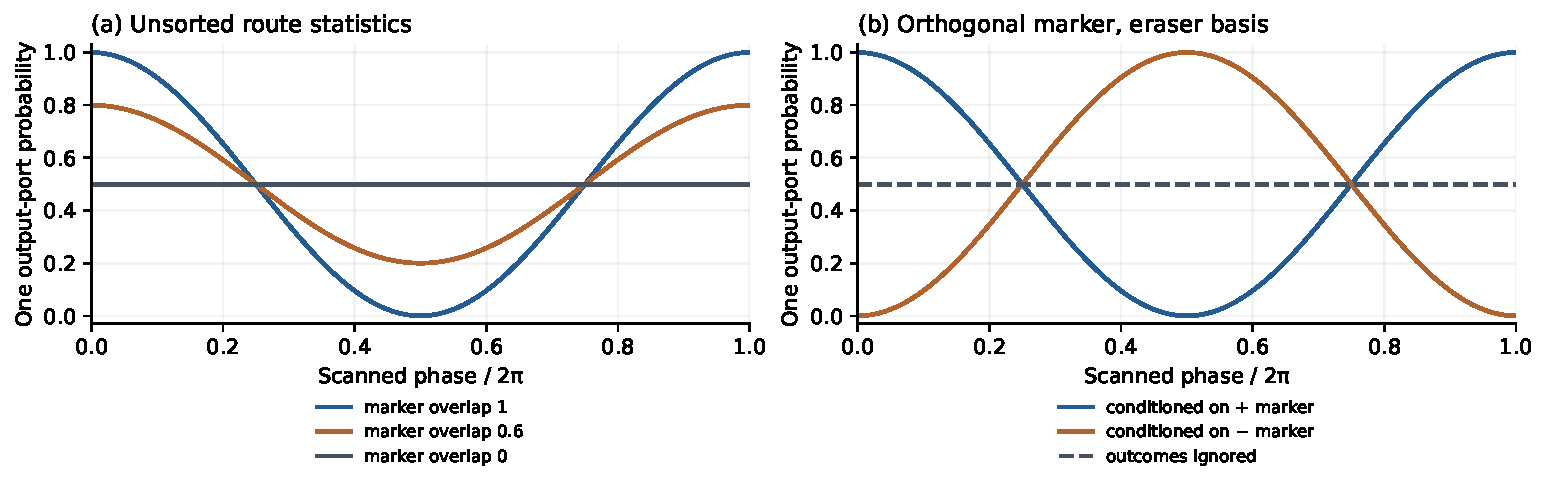
\includegraphics[width=.9\textwidth]{vi_source/record_fringes.pdf}
\caption{Exact balanced two-route comparator. (a) Real marker overlap changes unsorted interference through $P_+=(1+\gamma\cos\varphi)/2$. (b) For orthogonal markers, measuring the complementary marker basis gives two conditional fringes, each with probability one half. Ignoring that outcome yields the unchanged flat marginal. These analytic finite-system curves illustrate the stated protocol; they are not measured SAM data or an original-field simulation.}
\label{fig:record-fringes}
\end{figure*}
\subsection{Distinguishability, with the priors retained}
Consider the operational task of guessing a route from its marker, given priors $p,q$. For any binary POVM $E_0,E_1$ on $M$,
\begin{equation}
\begin{gathered}
P_{\rm guess}=p\,\operatorname{Tr}(E_0\rho_0)
          +q\,\operatorname{Tr}(E_1\rho_1),
 \\
 \rho_j=|m_j\rangle\langle m_j|.
\end{gathered}
\end{equation}
Set $H=p\rho_0-q\rho_1$. Since $E_1=I-E_0$,
maximizing $q+\operatorname{Tr}(E_0H)$ selects the positive spectral subspace of $H$. Hence
\begin{equation}
\begin{gathered}
P_{\rm guess}^{\rm opt}=\tfrac12(1+D),
 \\
 D=\|p\rho_0-q\rho_1\|_1 .
\end{gathered}
\label{eq:weighted-helstrom}
\end{equation}
This is weighted Helstrom distinguishability,\cite{BarnettCroke2009} not the unweighted trace distance unless $p=q=1/2$. On the span of the two pure markers, $\operatorname{Tr}H=p-q$ and
$\det H=-pq(1-|\gamma|^2)$. The two eigenvalues have opposite signs or one is zero, so
\begin{equation}
\begin{gathered}
D=\sqrt{1-4pq|\gamma|^2},\\
 D^2+V^2=1.
\end{gathered}
\label{eq:record-duality}
\end{equation}
Identical marker states give $D=|p-q|$: success then comes only from the prior imbalance. Orthogonal markers give $D=1$, $V=0$. Equation~\eqref{eq:record-duality} is an equality for this pure joint state with full marker access and the specified analyser. It is not an unrestricted equality for every apparatus. It belongs to the established two-way duality framework; see Englert.\cite{Englert1996}

There is a short general proof of the relevant inequality. Let $\rho_{SM}$ be any joint state and purify it with $E$. For $0<p<1$ the purification can be written
\begin{equation}
 |\Omega\rangle=\sqrt p\,|0\rangle|u\rangle_{ME}
                 +\sqrt q\,|1\rangle|v\rangle_{ME},
\end{equation}
with normalized conditional vectors. If $c=\langle0|\rho_S|1\rangle$, then $c=\sqrt{pq}\langle v|u\rangle$ and the same analyser gives $V=2|c|$. Weighted pure-state discrimination on $ME$ gives
$D_{ME}=\sqrt{1-4|c|^2}$. Partial trace is a trace-norm contraction on Hermitian operators, yielding
\begin{equation}
\begin{gathered}
D_M\leq D_{ME},\\
 D_M^2+V^2\leq1.
\end{gathered}
\label{eq:mixed-duality}
\end{equation}
The endpoints $p=0,1$ follow directly. This proof also covers a restricted accessible subsystem of the marker. It does not license comparing visibility in one postselected ensemble with distinguishability in another. These are the standard channel and discrimination conventions.\cite{Watrous2018}

\subsection{Reversal, erasure, and inaccessible markers}
An exact reversible two-qubit fixture uses $|m\rangle=|0\rangle$,
$U_0=I$, and
\begin{equation}
 U_1=R(\alpha)=\begin{pmatrix}
 \cos\alpha&-\sin\alpha\\ \sin\alpha&\cos\alpha
 \end{pmatrix}.
\end{equation}
Then $\gamma=\cos\alpha$. At $p=1/2$, $V=|\cos\alpha|$ and $D=|\sin\alpha|$. At $\alpha=\pi/2$ the marker is orthogonal and the reduced route state has no coherence. Applying the \emph{joint controlled inverse} $U^\dagger$ before analysis restores $|\psi\rangle|0\rangle$ and the original visibility. This is a reversal of the correlation-generating interaction. A marker-only unitary cannot accomplish it, since it preserves $\langle m_1|m_0\rangle$.

A quantum eraser is a different operation. For the orthogonal marker, measure $M$ in $|\!\pm\rangle_M=(|0\rangle\pm|1\rangle)/\sqrt2$. Each outcome has probability $1/2$ and prepares the conditional route state
\begin{equation}
 |\psi_\pm\rangle=\sqrt p\,|0\rangle
                   \pm e^{i\phi}\sqrt q\,|1\rangle .
\end{equation}
Its fringe visibility is $2\sqrt{pq}$, but the two fringes are shifted by $\pi$. Averaging their distributions cancels the interference. Conditional coincidence sorting requires the marker outcome; it does not restore an unconditional remote fringe. Outcome-dependent feed-forward can align the phases, but uses a communicated outcome and an operation on $S$. This distinction is central to the original quantum-eraser proposal of Scully and Dr\"uhl and to conditional coincidence experiments.\cite{ScullyDruhl1982,Kim2000}

Environmental copies constrain reversal. For branch states of the factorized form $|m_j\rangle|e_j\rangle$, the coherence multiplier is
\begin{equation}
 \gamma_{ME}=\langle m_1|m_0\rangle
                  \langle e_1|e_0\rangle .
\end{equation}
Reversing the controlled $S$--$M$ coupling while leaving $E$ intact does not remove the environmental factor. Orthogonal $|e_j\rangle$ maintain zero local coherence even when $E$ is inaccessible. Generic environmental states need not factorize; the purification argument above replaces this product formula in that case. No assertion about a gravitational horizon follows merely from tracing out $E$.

More generally, let $\Lambda_M$ be any trace-preserving local channel, including an unread measurement or reset. For every bipartite state,
\begin{align}
 \rho'_S&=\operatorname{Tr}_M[(I\otimes\Lambda_M)(\rho_{SM})]
            =\rho_S,\\
 T(\rho'_S,\rho_S)&=\tfrac12\|\rho'_S-\rho_S\|_1=0.
\end{align}
The equality follows from $\Lambda_M^*(I)=I$: every local expectation on $S$ is unchanged. Thus no route-only POVM can reveal the remote channel choice. Selective outcomes can change a conditional state, but the selection information must be transmitted. This is the precise no-signalling control on any proposed accessibility or erasure narrative.

\subsection{A durable accessible record is an operational claim}
A useful record definition specifies more than entanglement. Let $\{\mathcal I_j\}$ be a quantum instrument: each map is completely positive and trace non-increasing, and $\sum_j\mathcal I_j$ is trace preserving. Its probabilities are $p_j=\operatorname{Tr}\mathcal I_j(\rho)$, and its conditional output is $\mathcal I_j(\rho)/p_j$ for $p_j>0$. The instrument can describe a declared path-marking task, but must not be read as establishing a pre-existing route value in every coherent preparation. If only selected outcomes are retained, the omitted outcomes must remain in the complete instrument; renormalizing the retained branch describes postselection, not a new unconditional probability law.

For a proposed memory $R$, declare (i) the operational labels $j$, (ii) the conditional memory states $\sigma_R^j$, (iii) the storage dynamics $\mathcal N_t$, (iv) the channel $\mathcal A_{\mathcal D,t}$ delivering data to domain $\mathcal D$, and (v) an allowed decoder POVM $\{F_j(t)\}$. Call it an $(\epsilon,T)$ readable record for that domain when a predeclared physically implementable decoder satisfies
\begin{equation}
 \inf_{0\leq t\leq T}\ \min_{j:p_j>0}
 \operatorname{Tr}\!\left[F_j(t)
 \mathcal A_{\mathcal D,t}\mathcal N_t(\sigma_R^j)\right]
 \geq1-\epsilon .
 \label{eq:operational-record}
\end{equation}
Here $0\leq\epsilon<1/2$ for a binary record. The minimum over labels prevents a strongly biased source from passing by always guessing the common label. The time origin is the end of writing, and the interval tests one read performed at any chosen time; repeated non-destructive reading requires an additional back-action specification. Fixed decoders are a valid special case. Access may incorporate transport delay, controllable operations, or a restricted measurement algebra; the protocol must state which. Without those declarations, ``accessible'' is not a quantitative physical property.

Four different statements must remain separate. Entanglement concerns the joint state. Decoherence concerns suppressed off-diagonal terms in a specified reduced state and basis. A single registered outcome is described operationally by an instrument and the Born rule. A persistent readable record additionally passes Eq.~\eqref{eq:operational-record}. Unitary correlation and partial trace alone do not select one unique global outcome or solve the measurement problem.\cite{Schlosshauer2005} Nor does a record require awareness: every element of the definition is a physical preparation, channel, or decoder.

\subsection{Controls and the boundary of the claim}
The preceding equations prescribe concrete wrong-controls. Treating a marker-only rotation as a joint inverse incorrectly predicts an unconditional restored fringe. Tracing out an orthogonal environmental marker and then declaring it absent incorrectly reinstates coherence. Sorting eraser outcomes and comparing that conditional visibility with unsorted which-way data mixes ensembles. Treating $D$ as marker-acquired information without subtracting or reporting prior predictability misreads biased preparations. Treating a returned local state as a globally erased event discards the history carrier. Finally, labelling a reduced density matrix as one selected outcome imports an additional postulate without saying so.

These controls are standard quantum benchmarks. They discipline the route/write terminology and identify what an executable substrate account must reproduce. No new SAM prediction follows from renaming the instrument outcome a write. Such a prediction would require an additional, quantitatively specified dynamics or access rule, its parameter domain, and an experiment separating it from the retained quantum premises.


\section{Readable records and retained route coherence}
\label{sec:chvif-readable-records}

The following statements use the quantum state, channel, and measurement
premises already declared in Chapter VI. They make the relation between a
readable record and an unsorted interference experiment quantitative. The
record labels must refer to the same routes and the same ensemble as the
visibility; a reliable record of an unrelated label supplies no such bound.

\subsection{A same-state, worst-label theorem}
\label{sec:chvif-record-visibility-theorem}

Let $S$ be the two-route system and let $M$ contain the remaining physical
marker degrees of freedom. At the chosen observation time write an arbitrary
normalized joint state as
\begin{equation}
\begin{gathered}
\rho_{SM}=\sum_{j,k=0}^{1}|j\rangle\langle k|\otimes R_{jk},
 \\
 p=\operatorname{Tr}R_{00},\quad q=\operatorname{Tr}R_{11}=1-p.
\end{gathered}
\label{eq:chvif-record-block-state}
\end{equation}
For $p,q>0$, the conditional marker states are
$\sigma_M^0=R_{00}/p$ and $\sigma_M^1=R_{11}/q$. Their labels specify
the two diagonal route alternatives used by this operational test; this
notation does not select a unique outcome in a coherent joint state.

Declare a label-independent channel $\Lambda_t:M\longrightarrow D$ that
includes the storage and access operations available to the reading domain
at time $t$. It is completely positive and trace preserving, and acts on
the marker rather than on $S$. Let $F_0(t),F_1(t)$ be one physically
allowed decoder POVM on $D$, with $F_0+F_1=I_D$. The decoder may depend
on the declared time and controls, but receives no copy of the unknown
label. Define
\begin{equation}
\begin{gathered}
\tau_D^j(t)=\Lambda_t(\sigma_M^j),\\
 r_j(t)=\operatorname{Tr}[F_j(t)\tau_D^j(t)].
\end{gathered}
\label{eq:chvif-decoder-conditional-success}
\end{equation}
Storage and access can instead be specified jointly on an enlarged marker
containing a correlated environment, a transport carrier, and retained
classical records. No product-state or independent-noise assumption is
required. An environment correlated with the marker must be included in
that joint channel description when the proposed reduced channel would
otherwise depend on its correlations. Conditional states for the theorem
are always the actual conditional states of
Eq.~\eqref{eq:chvif-record-block-state} under that description.

Let $c=\langle0|\rho_S|1\rangle$. For a lossless two-route preparation
and the declared balanced, variable-phase analyser, with no
outcome-dependent filtering, the unsorted single-port visibility is
\begin{equation}
 V=2|c|.
 \label{eq:chvif-unsorted-record-visibility}
\end{equation}
The local, unselected channel $\Lambda_t$ does not change $\rho_S$.
Consequently a decoder can be analysed on $D$ while the visibility refers
to this same route marginal. A joint controlled inverse or feed-forward
operation on $S$ would define a different experiment and must be included
before applying the theorem to its resulting state.

\paragraph{Theorem.}
If, at the chosen time, both conditional decoder successes satisfy
\begin{equation}
\begin{gathered}
\min\{r_0(t),r_1(t)\}\geq1-\varepsilon,
 \\
 0\leq\varepsilon<\tfrac12,
\end{gathered}
\label{eq:chvif-worst-label-readability}
\end{equation}
then
\begin{equation}
 \boxed{\begin{gathered}
 V\leq4\sqrt{pq\,\varepsilon(1-\varepsilon)}
       \leq2\sqrt{\varepsilon(1-\varepsilon)} .\end{gathered}}
 \label{eq:chvif-readable-visibility-bound}
\end{equation}
For balanced priors the two bounds agree. For unequal priors the first
retains their additional restriction on the fringe. At $p=0$ or $q=0$,
positivity already gives $c=0$ and $V=0$; a conditional success statement
about an absent label must be supplied by a separately declared calibration
preparation if it is wanted.

\paragraph{Derivation.}
Apply the decoder to $(I_S\otimes\Lambda_t)(\rho_{SM})$ and retain its
two outcomes. The unnormalized route state for outcome $y$ is positive,
with diagonal entries $p a_y,q b_y$, where
\begin{equation}
\begin{gathered}
a_y=\operatorname{Tr}[F_y\tau_D^0],\\
 b_y=\operatorname{Tr}[F_y\tau_D^1].
\end{gathered}
\end{equation}
If its off-diagonal entry is $c_y$, positivity of this $2\times2$ matrix
and preservation of the unselected marginal give
\begin{equation}
\begin{gathered}
|c_y|\leq\sqrt{pq\,a_yb_y},\\
 c=\sum_y c_y,
 \\
 |c|\leq\sqrt{pq}\sum_y\sqrt{a_yb_y}.
\end{gathered}
\label{eq:chvif-decoder-bhattacharyya}
\end{equation}
This argument retains arbitrary off-diagonal marker blocks and arbitrary
correlations with inaccessible degrees of freedom.

Put $a=a_1$ and $b=b_0$, the two conditional error probabilities. The
readability hypothesis gives $0\leq a,b\leq\varepsilon$, and the last
sum in Eq.~\eqref{eq:chvif-decoder-bhattacharyya} is
\begin{equation}
 \sqrt{(1-a)b}+\sqrt{a(1-b)}.
\end{equation}
Write $a=\sin^2\alpha$, $b=\sin^2\beta$, with
$0\leq\alpha,\beta\leq\arcsin\sqrt{\varepsilon}<\pi/4$. This sum is
$\sin(\alpha+\beta)$, hence it is at most
$2\sqrt{\varepsilon(1-\varepsilon)}$. Multiplying by $2\sqrt{pq}$ gives
Eq.~\eqref{eq:chvif-readable-visibility-bound}, including
$\varepsilon=0$ by continuity or direct substitution.

The weaker bound also follows immediately from weighted discrimination:
the stated decoder has prior-weighted success at least $1-\varepsilon$,
so $D_D=\|p\tau_D^0-q\tau_D^1\|_1\geq1-2\varepsilon$.
The same-state inequality $D_D^2+V^2\leq1$ then gives
$V\leq2\sqrt{\varepsilon(1-\varepsilon)}$. The
Bhattacharyya derivation uses both separate error constraints and therefore
retains the stronger prior-dependent factor. No optimal decoder needs to
be physically available: the actual allowed decoder in
Eq.~\eqref{eq:chvif-worst-label-readability} is enough.

\paragraph{Tight qubit example.}
For any $0\leq\varepsilon<1/2$, take
\begin{align}
 |m_0\rangle&=\sqrt{1-\varepsilon}|0\rangle
                      +\sqrt{\varepsilon}|1\rangle,\\
 |m_1\rangle&=\sqrt{\varepsilon}|0\rangle
                      +\sqrt{1-\varepsilon}|1\rangle,\\
 |\Psi\rangle&=\sqrt p\,|0\rangle|m_0\rangle
                 +e^{i\phi}\sqrt q\,|1\rangle|m_1\rangle.
 \label{eq:chvif-tight-record-qubits}
\end{align}
The computational-basis decoder succeeds with probability
$1-\varepsilon$ on each label, and
$\langle m_1|m_0\rangle=2\sqrt{\varepsilon(1-\varepsilon)}$.
Its visibility saturates the first bound in
Eq.~\eqref{eq:chvif-readable-visibility-bound} for every $p,q$.
For $\varepsilon=0$ the marker is perfectly readable and the route marginal
has zero visibility, while the pure joint state still retains its coherent
superposition. A later joint reversal can recover interference while
changing the record. The theorem bounds the specified unsorted fringe;
it does not identify loss of its contrast with deletion of global coherence.

\subsection{Arrival, retention, and the time of reading}
\label{sec:chvif-record-arrival}

An $(\varepsilon,W_D)$ readable record for domain $D$ requires the
worst-label condition at every allowed reading time $t\in W_D$, with
the channel, allowed decoder, and time origin declared. The theorem then
bounds the contemporaneous visibility at every such time for which the
same route/marker description applies. The statement concerns one read
at a chosen time. A sequence of reads requires the actual reading
instruments and their disturbance; the interval condition alone supplies
no nondestructive repeated-read guarantee.

There is a precise causal pre-arrival restriction. Suppose a newly encoded
label has no label-dependent receiver state in its causal past and the
declared channel has not delivered any label-dependent degree of freedom
by time $t$. Then
\begin{equation}
 \tau_D^0(t)=\tau_D^1(t)=\tau_D(t).
 \label{eq:chvif-before-arrival-states}
\end{equation}
Every binary decoder obeys $r_0+r_1=1$ on this common state, so
\begin{equation}
 \min_j r_j(t)\leq\tfrac12.
 \label{eq:chvif-before-arrival-no-record}
\end{equation}
Thus it cannot satisfy the declared $\varepsilon<1/2$ readability before
arrival. This conclusion needs the explicit identical-state premise,
provided physically by the causal/no-signalling access model. A receiver
that already holds a correlated copy of the label is a different resource
configuration. Unequal priors can improve an average guess before arrival,
but cannot pass the worst-label condition.

The storage window and receiver window are consequently different objects.
Let the end of writing be $t=0$, and suppose the stored encoding is
guaranteed at the memory for emission times $t_e\in[0,T_M]$. For a fixed
latency $\tau$ and a separately budgeted readout time $\tau_{\rm dec}$,
the corresponding idealized completion times are
\begin{equation}
\begin{gathered}
t_D=t_e+\tau+\tau_{\rm dec},\\
 W_D=[\tau+\tau_{\rm dec},\,
                         T_M+\tau+\tau_{\rm dec}].
\end{gathered}
\label{eq:chvif-memory-receiver-windows}
\end{equation}
This translated window assumes that the access channel actually samples
the memory at $t_e$ and that its transport, intervening storage, and decoder
errors have been paid. A protocol needing the memory throughout a finite
read instead requires that entire memory-side interval inside its retention
window. Variable travel times use the declared retarded emission map
$t_e(t_D)$ and its admissible interval. Starting a receiver guarantee at
the end of writing would incorrectly include times before delivery unless
delivery was already available. Choosing the domain time origin at
arrival is valid when that convention is stated.

\subsection{Composable error budgets and retained failed preparations}
\label{sec:chvif-record-composition}

Worst-label budgets compose without independent errors. One convenient
quantum formulation includes all classical outcome flags and relevant
environmental references in the joint state. Let the ideal decoder have
error at most $\varepsilon_0$ on each label. Suppose a hybrid comparison
of the actual preparation, storage, transport, and readout gives
trace-distance errors $\delta_k$ on the relevant joint conditional states
at stage $k$. Each stage bound must hold for the hybrid inputs actually
used, including retained correlations; an entangled reference is included
in the comparison when present. Equivalently, a uniform channel bound
can be supplied on that declared joint input class.

Contractivity under the subsequent trace-preserving channels and the
triangle inequality give a final joint-state distance at most
$\sum_k\delta_k$. A fixed POVM outcome probability changes by no more
than that distance. Consequently
\begin{equation}
\begin{gathered}
r_j^{\rm actual}(t)\geq
       1-\varepsilon_0-\sum_k\delta_k,
 \\
 \varepsilon_{\rm tot}=\varepsilon_0+\sum_k\delta_k.
\end{gathered}
\label{eq:chvif-additive-record-budget}
\end{equation}
The readability and visibility theorem applies when the declared total is
below $1/2$. Isolated marginal error estimates cannot be substituted for
these joint-state bounds when unaccounted correlations change the channel.
The hybrid channels and flags also preserve any feedback used by the
actual instrument.

A classical alternative is an explicit sequence of bad-event flags whose
conditional probability, on every reached prior history and each label,
is at most $\delta_k$. If the final decoder error on the all-good branch
is at most $\varepsilon_0$, the union bound gives the same additive
budget. This argument likewise needs no independence. It does need the
stated conditional bounds; adding unrelated average failure rates would
not establish a worst-label guarantee.

Preparation failure belongs in the full instrument. Suppose label $j$ has
failure probability $f_j\leq f$, and the successful preparation has
worst-label reading error at most $\varepsilon_{\rm succ}$. If an explicit
failure or abstention is counted as an unsuccessful attempted read, then
\begin{equation}
 r_j^{\rm attempt}\geq
       (1-f_j)(1-\varepsilon_{\rm succ})
       \geq1-f-\varepsilon_{\rm succ}.
 \label{eq:chvif-preparation-failure-record}
\end{equation}
Success, failure, and abstention flags remain in the normalized all-outcome
state and in the physical resource account. A larger decoder alphabet can
be retained explicitly, or its failure outcomes can be assigned a stated
binary guess without discarding them.

Alternatively a claim may be conditioned on a heralded success. Its
normalization, conditional record states, and conditional visibility must
then all use that same accepted ensemble. In a route-preserving heralded
preparation the accepted priors become
\begin{equation}
\begin{gathered}
p_{\rm acc}=\frac{p(1-f_0)}{p(1-f_0)+q(1-f_1)},\\
 q_{\rm acc}=1-p_{\rm acc},
\end{gathered}
\label{eq:chvif-accepted-record-priors}
\end{equation}
when the denominator is positive. Outcome-dependent filtering can also
change the coherence, so the accepted joint state itself must be used.
A conditional high-visibility ensemble cannot be compared with a readable
record certified only in a different, unselected ensemble. No reset of
failed preparations or deletion of their records is supplied by this
probability accounting.

\subsection{A finite readable-label capacity consequence}
\label{sec:chvif-record-capacity}

For $N$ declared labels, suppose the full accessible record input has
finite Hilbert dimension $d$ and one POVM $\{F_j\}_{j=1}^N$ satisfies
$\operatorname{Tr}(F_j\sigma_j)\geq1-\varepsilon$ for every normalized
conditional state $\sigma_j$. Since $0\leq\sigma_j\leq I$,
\begin{equation}
 N(1-\varepsilon)
    \leq\sum_{j=1}^N\operatorname{Tr}(F_j\sigma_j)
    \leq\sum_{j=1}^N\operatorname{Tr}F_j=d.
 \label{eq:chvif-approx-readable-capacity}
\end{equation}
Thus $d\geq\lceil N(1-\varepsilon)\rceil$. Any correlated side carrier
available to the decoder belongs in that accessible dimension; alternatively
the decoder is pulled back to a POVM on the declared input space. This
bound concerns $N$ physically decodable labels. Merely naming additional
ordered histories does not add distinguishable record states. It assigns
neither an energy per label nor a thermal erasure cost.


% Chapter VI component. Standard LaTeX + amsmath, amssymb only.
% Self-contained finite-dimensional proofs; no external theorem package required.
\section{Restoration of a local state and retention of a physical history}
\label{sec:restoration-history}

The source interface is
\begin{equation}
 W8+X1\longrightarrow W9\longrightarrow W8'.
 \label{eq:write-interface}
\end{equation}
Here $W8$ names the resting, non-contact local substrate state; $X1$
names the supplied interaction; and $W9$ names the temporary write state.
The prime marks return after interaction, not a new substrate atom.
The source's intended distinction is that a local state can return while
an event remains recorded elsewhere. This section gives that distinction
an explicit quantum-information comparator. It does not identify the
symbols $W8$, $X1$, and $W9$ with Hilbert-space dimensions, derive their
exact SAM/SLC grammar, or prove a substrate microdynamics.

Chapter II already distinguishes an address from the history of its use.
Returning to a retained address does not by itself say whether a record
survives. Nor does a finite alphabet supply unlimited storage: a physical
history requires distinguishable states of some specified recipient.
The same discipline applies here. We must name the restored subsystem,
the other degrees of freedom, and the operations by which a record can
be read.

\subsection{What a unitary reset can and cannot do}
\label{subsec:reset-theorem}

Let $L$ be a local record cell and let $E$ include every other degree of
freedom participating in a closed finite-dimensional evolution. Suppose
$\{|m_i\rangle_L\}_{i=1}^n$ are orthonormal pointer states and $E$ starts
in a fixed pure state $|e_0\rangle$. An exact reset of $L$ has the form
\begin{equation}
 U\bigl(|m_i\rangle_L|e_0\rangle_E\bigr)
   =|0\rangle_L|e_i\rangle_E.
 \label{eq:unitary-reset}
\end{equation}
\noindent\textbf{Reset--recipient proposition.}
If $U$ is unitary, then $\langle e_i|e_j\rangle=\delta_{ij}$.
Consequently $E$ cannot also return to one fixed state when $n>1$.
The recipient needs at least $n$ mutually orthogonal states.

\noindent\emph{Proof.}
Preservation of inner products gives
\begin{equation}
 \delta_{ij}
 =\langle m_i,e_0|m_j,e_0\rangle
 =\langle 0,e_i|0,e_j\rangle
 =\langle e_i|e_j\rangle.
\end{equation}
An exact pure local output factors from the rest, so this argument also
covers a purported reset whose output was initially written as a general
joint pure state. A mixed initial environment may be purified by adding
its reference to $E$; the conclusion then concerns that enlarged
recipient. It does not guarantee a record readable from an arbitrarily
chosen proper part of $E$. $\square$

There is an important scope condition. If a separate system $S$ already
contains a correlated copy, the input is not the fixed-environment input
of Eq.~\eqref{eq:unitary-reset}. In the more general pure-state mapping
\begin{equation}
 |s_i\rangle|m_i\rangle|e_0\rangle
 \longmapsto |s_i'\rangle|0\rangle|e_i\rangle,
\end{equation}
unitarity requires, for $i\ne j$,
\begin{equation}
 \langle s_i'|s_j'\rangle\langle e_i|e_j\rangle=0.
 \label{eq:reset-factor}
\end{equation}
If $S$ returns to one common pure state, the recipient states must be
orthogonal. If $S$ instead retains orthogonal alternatives, it can itself
carry the distinction; a new record in $E$ is not compulsory. For example,
reversing a controlled write resets the cell while retaining the source
bit. The assertion that ``every reset must write a new history register''
would therefore be false. The invariant is distinguishability of the
complete closed state, not the permanence of a selected local mark.
For mixed or entangled subsystems, surviving information may be in joint
correlations rather than readable in any one marginal.

\subsection{Three registers: a write, a restoration, and a retained marker}
\label{subsec:three-register-write}

Use three qubits: route $S$, local cell $L$, and history recipient $H$.
The history register is initially blank. Define
\begin{equation}
\begin{gathered}
C|r,\ell,h\rangle=|r,\ell\mathbin{\oplus}r,h\rangle,
 \\
 T=\operatorname{SWAP}_{LH},
\end{gathered}
\end{equation}
where $r,\ell,h\in\{0,1\}$ and $\oplus$ is addition modulo two.
Both maps permute the full eight-state computational basis, so both
are unitary without a restriction to the intended input states.
Their composition is
\begin{equation}
\begin{gathered}
U=TC,\\
 U|r,\ell,h\rangle
     =|r,h,\ell\mathbin{\oplus}r\rangle.
\end{gathered}
\label{eq:three-register-unitary}
\end{equation}
For a normalized coherent route input,
\begin{align}
 |\Psi_{\rm in}\rangle
  &=(\alpha|0\rangle+\beta|1\rangle)_S|0\rangle_L|0\rangle_H,
  \nonumber\\
 |\Psi_{\rm write}\rangle
  &=\alpha|000\rangle+\beta|110\rangle,
  \label{eq:write-stage}\\
 |\Psi_{\rm restored}\rangle
  &=\alpha|000\rangle+\beta|101\rangle
  \nonumber\\
  &=|0\rangle_L\bigl(\alpha|00\rangle_{SH}
                        +\beta|11\rangle_{SH}\bigr).
 \label{eq:restored-stage}
\end{align}
The local cell is exactly restored. Conditioned on the route alternative,
the history states are $|0\rangle_H$ and $|1\rangle_H$, which can be
perfectly discriminated. For a coherent input, however, the final state
is an entangled superposition, not a derivation of one selected outcome.
The comparator exhibits a readable pointer correlation and local
restoration. It does not derive collapse or a unique realized history.

The analogy to Eq.~\eqref{eq:write-interface} is deliberately limited:
resting cell, interaction-enabled write, restored cell with a retained
recipient correlation. The interaction $X1$ is not treated as an extra
qubit or an arithmetical increment. The temporary $W9$ designation may
refer to the interaction configuration; it need not mean that the cell
alone has changed in every branch. In particular, the $r=0$ branch leaves
its pointer value at zero even during the controlled write.

The inverse exists on every input: $U^{-1}=C T$. With joint control of
$S,L,H$, it returns Eq.~\eqref{eq:restored-stage} to
$|\Psi_{\rm in}\rangle$. The phase information was never deleted from
the complete state. By contrast, tracing out the record gives
\begin{equation}
 \rho_S=|\alpha|^2|0\rangle\langle0|
          +|\beta|^2|1\rangle\langle1|
 \label{eq:restored-route-marginal}
\end{equation}
both after the write and after the restoration. Thus the swap does not
restore route-only interference. Global coherence is preserved throughout;
its observability depends on access to the correlated degrees of freedom.
Joint reversal, or suitable measurements of the record with conditioned
route statistics, can reveal that coherence. An operation on the
inaccessible record alone cannot change the unconditioned route marginal.

For example, take $\alpha=1/\sqrt2$ and $\beta=e^{\mathrm{i}\phi}/\sqrt2$.
The joint observable $X_S X_H$ has expectation $\cos\phi$ after restoration,
whereas every route-only expectation is independent of $\phi$.
This is the precise distinction between preservation in the closed system
and accessibility in a restricted domain.

This device stores one binary marker. It does not store an arbitrary
sequence of writes. If $H$ is already occupied, the swap returns that
previous content to $L$, rather than resetting $L$ to zero. Repeated
restoration needs additional blank capacity, a deliberate reversible
compression when possible, or an explicitly modeled disposal channel.
Perfectly distinguishing $N$ possible complete histories requires $N$
orthogonal global record states and hence a record-space dimension at
least $N$. This is a storage statement, not a heat formula.

\subsection{Pointer copying is not universal quantum cloning}

For a declared orthogonal pointer basis, a controlled operation can copy
its label:
\begin{equation}
 |r\rangle|0\rangle\longmapsto |r\rangle|r\rangle.
\end{equation}
Applied to a superposition, it creates the correlated state in
Eq.~\eqref{eq:write-stage}; it does not produce two copies of
$\alpha|0\rangle+\beta|1\rangle$. Indeed, let the overlap of two normalized inputs be $z$ and allow the
cloner to finish in input-dependent auxiliary states $|a_\psi\rangle$ and
$|a_\varphi\rangle$. Inner-product preservation would require
$z=z^2\langle a_\psi|a_\varphi\rangle$. For $0<|z|<1$, this implies
$1\le |z|$, a contradiction. Universal cloning is therefore impossible
even when the auxiliary state is allowed to change.

Transfer is different. A swap implements
\begin{equation}
 |\psi\rangle_L|0\rangle_H\longmapsto
 |0\rangle_L|\psi\rangle_H
\end{equation}
for every $|\psi\rangle$, preserving its entanglement with any reference.
The input remains present once, at its new location. Resetting $L$
while leaving both the recipient and all other degrees of freedom fixed
would instead delete an unknown input, contrary to inner-product
preservation. These elementary statements suffice for this interface;
no universal copying or unexplained destruction of quantum information is being assumed. Related no-deleting and no-hiding results have their own hypotheses; no claim that information must reside only in correlations is used here.\cite{PatiBraunstein2000,BraunsteinPati2007}

\subsection{A physical record needs an accessible decoder}
\label{subsec:accessible-decoder}

The decoder criterion of Eq.~\eqref{eq:operational-record} applies to the nominated recipient, not merely the restored cell. For equal priors, the three-register example has trace distance one between its conditional history states and zero between its conditional local-cell states. The history permits perfect route decoding; the restored cell permits only chance performance. The Helstrom optimum is attainable only if its measurement belongs to the allowed set.

Durability adds a time and noise specification. A useful requirement is
that a stated decoder recover the label with error at most $\epsilon$
after a declared storage interval and channel. Orthogonality at the moment
of writing does not by itself establish durability. For example, encoding
a classical bit in an odd number $n$ of identical pointer cells and
reading by majority vote gives
\begin{equation}
\begin{gathered}
P_{\rm err}\le
 \exp\{-2n(\tfrac12-p)^2\},\\
 p<\tfrac12,
\end{gathered}
\end{equation}
if, conditional on the stored bit, the cell errors are independent and
each has probability at most $p$. For error indicators $E_j$ and $t=1/2-p>0$, independence and the
bounded-variable exponential-moment inequality give
\begin{equation}
 \Pr\!\left\{\sum_j(E_j-\mathbb E E_j)\ge nt\right\}
 \le \inf_{\lambda>0}e^{-\lambda nt+n\lambda^2/8}
 =e^{-2nt^2}.
\end{equation}
Majority failure is contained in the displayed event. Correlated failures need not satisfy it: one
common flip of all cells leaves a majority decoder with the same error
probability as a single cell. This example is an optional classical
storage mechanism, not a derived SAM durability law.

Finally, a history description is not an additional quantum observable.
If two proposed histories yield the same accessible density operator,
every accessible POVM gives the same outcome probabilities. Calling one
state $W8$ and the other $W8'$ cannot change this. If a history can be
read, its evidence must reside in distinguishable accessible states or
correlations, with a specified decoding operation. This is the physical
content of the prime: local return is compatible with a retained record,
but the notation alone neither guarantees that record nor makes it
accessible.

No thermodynamic cost is inferred from these unitary maps. A Landauer
bound belongs to a separately declared cyclic erasure protocol with a
thermal reservoir, temperature, initial logical ensemble, and work/heat
accounting. Neither the number of local addresses nor the logarithm of a
record-space dimension is, by itself, dissipated heat. The present result
is narrower: a local restoration can transfer a physical distinction;
it cannot establish the disappearance of that distinction from a closed
unitary account.


\section{The original interacting clock on coherent routes}
% Chapter VI: original interacting source, conditional proper-time interface.
\subsection{The full interacting source as a route marker}
\label{sec:ch6-clock-routes}
A route-dependent clock requires a receiving rule connecting the local
interacting dynamics to spacetime transport. The following rule is conditional~\cite{Zych2011}:
the same isolated, co-moving source--field Hamiltonian acts along each prescribed
timelike route, with its Chapter I time chart replaced by accumulated proper
time. External beam splitters, recombination, routing forces, and the spacetime
geometry are controls; they are not derived from the source Hamiltonian.
Tidal changes of the internal Hamiltonian, radiation caused by the controls,
and inaccessible environmental records require additional terms or a larger
marker system. A field shared nonlocally by both arms does not automatically
admit this isolated co-moving reduction.

Retain the complete source space $\mathbb C^4\otimes\mathbb C^4$ and the two
polarizations of the continuum Fock field. In the Chapter I dimensionless
chart the rest generator is
\begin{equation}
\begin{split}
 H_0={}&\epsilon(S+Q_L+Q_R+Q_LQ_R)+H_f\\
 &-\epsilon(D\phi_++C\phi_\times)\\
 &+\epsilon^2\mu(D^2+C^2),\\
 D={}&Q_L-Q_R,\qquad C=iSD,\qquad \mu=(4R)^{-1}.
\end{split}
\label{eq:ch6-full-clock-generator}
\end{equation}
This is the original interacting form-sum Hamiltonian, not a bare two-level
substitution. Its six two-state lanes and four unforced diagonal states are
all retained. In a chosen prepared lane $a<b$, $d=q_a-q_b<0$,
$g=\epsilon d$, and the restriction is
$H_0=\epsilon eI+\epsilon S+H_f-g(\sigma_z\phi_++\sigma_y\phi_\times)+cI$,
where $e=q_a+q_b+q_aq_b$ and $c=2g^2\mu$. Both the even energy and the two
counterterms remain in the generator.

For route $j$, define
\begin{equation}
 \begin{gathered}
 \eta_j=s_0\int_{\gamma_j}d\tau_{\rm proper},\qquad
 U_j=e^{-iH_0\eta_j},\\
 U_{\rm ctrl}=\sum_{j=1}^2|j\rangle\langle j|\otimes U_j.
 \end{gathered}
 \label{eq:ch6-controlled-clock}
\end{equation}
Here $s_0=1/t_u$ in the declared Chapter I chart; no new SI calibration is
inferred. With $I_*=\hbar$, the physical rest energy
is $(\hbar/t_u)H_0$. Conditional on this transport law, the actual clock
coordinate obeys $d\theta/dt=\nu(\eta_j)(d\tau_{\rm proper}/dt)/t_u$ wherever
its certified inverse exists. This does not extend the Chapter I finite-window
rate certificate beyond its stated preparation and interval.

Let the route input be $\sqrt{p_1}|1\rangle+e^{i\alpha}\sqrt{p_2}|2\rangle$,
$p_1+p_2=1$, initially uncorrelated with a marker state $\rho$. Tracing the
marker gives route coherence proportional to
\begin{equation}
\begin{gathered}
\Gamma(\delta\eta)=\operatorname{Tr}(\rho U_2^\dagger U_1)
 =\operatorname{Tr}(\rho e^{-iH_0\delta\eta}),\\
 \delta\eta=\eta_1-\eta_2.
\end{gathered}
\label{eq:ch6-route-overlap}
\end{equation}
An ideal variable-phase recombiner measures fringe visibility
$\mathcal V=2\sqrt{p_1p_2}|\Gamma|$. The standard Born measurement rule is assumed in this calculation, not
derived from the original Write histories. The phase of $\Gamma$ shifts the fringes;
its modulus controls their contrast. Extra uncontrolled route records multiply
or otherwise modify this coherence and must be included explicitly.

For balanced priors, the operational which-route distinguishability in the
full marker is
\begin{equation}
\begin{gathered}
\mathcal D=\tfrac12\|U_1\rho U_1^\dagger-U_2\rho U_2^\dagger\|_1,
 \\
 \mathcal D^2+|\Gamma|^2\leq1.
\end{gathered}
\label{eq:ch6-duality}
\end{equation}
Equality holds for a pure initial full marker with unrestricted joint
measurements. For a mixed marker the inequality follows by purifying $\rho$:
the two purified states have overlap $\Gamma$, and partial trace contracts
trace distance. Restricted access to the source alone can only decrease
$\mathcal D$. For unequal priors the corresponding statement uses
$\|p_1\rho_1-p_2\rho_2\|_1$ and $\mathcal V$.
In particular, if $[\rho,H_0]=0$, then $\rho_1=\rho_2$ and $\mathcal D=0$,
although $|\Gamma|$ may be small. Mixed-state phase averaging is not itself
accessible which-route information in that marker. Nor does the phase-clock
expectation $z=\langle Z\rangle$ determine $\Gamma$: one is an expectation
of an evolved observable, the other a full-state propagator overlap.

\subsection{The needed spectral operand and its domain}
\label{sec:ch6-spectral-clock-operand}
Let $P_{H_0}$ be the spectral measure of the full interacting Hamiltonian.
The new original-source operand needed for exact route contrast is
\begin{equation}
\begin{gathered}
d\mathcal P_\rho(E)=\operatorname{Tr}[\rho P_{H_0}(dE)],\\
 \Gamma(s)=\int e^{-iEs}\,d\mathcal P_\rho(E).
\end{gathered}
\label{eq:ch6-spectral-operand}
\end{equation}
Chapter I's bounds on $M$, $\Omega$, $z$, and $\nu$ do not provide this
entire measure or the exact Loschmidt amplitude. A new spectral enclosure,
a controlled evaluation of this matrix element, or an overlap enclosure
with a stated error is needed for a numerical full-continuum fringe curve.
The matched hard mean energy $\bar E$ is also required for its absolute
reference phase; a gap enclosure alone does not determine that phase.

If $\int E^2d\mathcal P_\rho(E)<\infty$, set
$\sigma_H^2=\int(E-\bar E)^2d\mathcal P_\rho(E)$. Then
\begin{equation}
\begin{gathered}
|\Gamma(s)|^2=1-\sigma_H^2s^2+o(s^2),\\
 |\Gamma(s)|=1-\tfrac12\sigma_H^2s^2+o(s^2).
\end{gathered}
\label{eq:ch6-short-time-contrast}
\end{equation}
These coefficients use the full prepared joint-energy distribution.
Neither the bare exchange gap $2\epsilon$ nor the calibration expectation
$E_{\rm ref}=573049$ is an energy variance. The latter belongs to a different
placement-basis calibration preparation. For a pure state the requisite
condition is $\Psi\in D(H_0)$, not merely the energy form domain
$D(H_f^{1/2})$. Chapter I explicitly has ultraviolet-divergent
$\int_0^\infty|u_R|^2d\omega$; consequently a generic bare vacuum argument
cannot supply this second moment.

When this finite-variance condition holds, the standard quantum speed
bound~\cite{Fleming1973,DeffnerCampbell2017} follows because the projective Hilbert-space
speed of a purification evolving under $H_0$ is $\sigma_H$. Thus
\begin{equation}
\begin{aligned}
 \arccos|\Gamma(s)|&\leq\sigma_H|s|,\\
 |\Gamma(s)|&\geq\cos(\sigma_H|s|),
 \quad \sigma_H|s|\leq\pi/2.
\end{aligned}
 \label{eq:ch6-speed-bound}
\end{equation}
Any zero of the amplitude requires $|s|\geq\pi/(2\sigma_H)$.
For a mixed initial marker this is a bound on the specified amplitude (or its
purification), not a claim that the reduced marker becomes distinguishable
at that time. The full pure-state marker also obeys
$\mathcal D\leq\sin(\sigma_H|s|)$ on this interval.

\paragraph{A finite full-H second moment for the actual declared preparation.}
The ultraviolet qualification does not invalidate the particular hard-branch
preparation that Chapter I actually declares. Let $H_{\rm ref}$ be its
matched hard-interacting Hamiltonian, with the same even scalar and soft
counterterm as $H_0$, and let
\begin{equation}
\begin{aligned}
 \psi_k&=\Phi_k\otimes|0_s\rangle,
 &\Psi_0&=(\psi_0+\psi_1)/\sqrt2,\\
 H_{\rm ref}\psi_k&=E_k\psi_k,
 &E_1-E_0&=\Omega.
\end{aligned}
\end{equation}
The normalized exact hard eigenvectors are operator-domain vectors of their
hard Hamiltonian. The reference preparation is therefore in
$D(H_{\rm ref})$. Write
\begin{equation}
\begin{aligned}
 V_s&=H_0-H_{\rm ref}\\
    &=-g(\sigma_z\phi_{+,s}+\sigma_y\phi_{\times,s}),\\
 v_s&=\int_0^\lambda|u_R(\omega)|^2\dd\omega
 \leq v_s^{\rm up}=\frac{R^4\lambda^6}{675\kappa\pi}.
\end{aligned}
\end{equation}
On this soft vacuum, $V_s\Psi_0$ is a Hilbert-space vector with exactly one
soft photon. The two polarization insertions are orthogonal and both Pauli
operators preserve norm, giving $\|V_s\Psi_0\|^2=2g^2v_s$.
The form identity against every test vector in the common form domain is
represented by the Hilbert vector $H_{\rm ref}\Psi_0+V_s\Psi_0$.
The representation theorem for the closed form therefore proves
$\Psi_0\in D(H_0)$ and $H_0\Psi_0=H_{\rm ref}\Psi_0+V_s\Psi_0$.
Orthogonality of zero and one soft photon sectors now gives the new exact
identity
\begin{equation}
\begin{gathered}
\bar E=\tfrac12(E_0+E_1),\\
 \boxed{\ \sigma_H^2=\frac{\Omega^2}{4}+2g^2v_s\ }
 \leq\frac{\Omega^2}{4}+2g^2v_s^{\rm up}.
\end{gathered}
\label{eq:ch6-prepared-full-variance}
\end{equation}
This is a full interacting variance, despite its expression in matched
reference data. It relies on the exact hard eigenbranch preparation; it is
not a general domain assertion about arbitrary coherent source states.
It also does not assert $\Psi_0\in D(H_0^2)$ or existence of higher moments.
The signed $g$ is retained in the Hamiltonian; its square appears here because
this is a norm. A rigorous numerical speed enclosure follows by using the
original certificate's upper bounds for $\Omega$, $|g|$, $R$, and $\lambda$,
with their declared dependencies, rather than rounded lane numbers.

\paragraph{Six-lane consequences of the retained inputs.}
Table~\ref{tab:ch6-route-clock-bounds} uses the original rational enclosures
for $\Omega$, signed $g$, $v_s^{\rm up}$ and $T_0=2\pi/\Delta$.
The new rational operations are recorded in the companion check output;
each printed bound is verified outward by exact rational comparison.
These are independently derived enclosures, not a new native-certificate run.
The lower orthogonality ratio is slightly above one half in every lane,
while the reference-amplitude error at $T_0$ is at most $4.54\times10^{-11}$.
This does not imply that an exact zero or a perfect revival occurs.
\begin{table}[ht]
\centering\scriptsize
\begin{tabular}{c c c c}
\hline
Lane & $10^6\sigma_H$ upper & error at $T_0$ upper & $s_\perp/T_0$ lower\\
\hline
01 & 1.745051466079 & $1.759\times10^{-12}$ & 0.500000001207\\
02 & 1.745051452191 & $3.644\times10^{-12}$ & 0.500000005186\\
03 & 1.745048665211 & $4.536\times10^{-11}$ & 0.500000803726\\
12 & 1.745051465446 & $1.886\times10^{-12}$ & 0.500000001389\\
13 & 1.745048878445 & $4.360\times10^{-11}$ & 0.500000742629\\
23 & 1.745049097788 & $4.172\times10^{-11}$ & 0.500000679781\\
\hline
\end{tabular}
\caption{Full interacting hard-branch preparation: variance-speed and
matched-reference bounds. The error is an amplitude error, and $s_\perp$
is any first possible overlap zero, in the dimensionless proper-time chart.}
\label{tab:ch6-route-clock-bounds}
\end{table}

\paragraph{An independent overlap enclosure from the same preparation.}
The reference overlap is
$\Gamma_{\rm ref}(s)=e^{-i\bar Es}\cos(\Omega s/2)$.
The reference orbit is a finite sum of operator-domain eigenvectors, and its soft insertion is Hilbert-space continuous. Strong Hilbert-space Duhamel, with the full interacting propagator left intact, gives
\begin{equation}
\begin{aligned}
 &\|(e^{-isH_0}-e^{-isH_{\rm ref}})\Psi_0\|\\
 &\quad\leq\int_0^{|s|}\|V_s e^{-iuH_{\rm ref}}\Psi_0\|\dd u
 =|s|\sqrt{2g^2v_s}.
\end{aligned}
\end{equation}
The same orthogonal soft-sector norm is constant for every reference time;
negative $s$ is handled by reversing the integral. Consequently
\begin{equation}
\begin{aligned}
 \varepsilon_s&=|s|\sqrt{2g^2v_s^{\rm up}},\\
 |\Gamma(s)-e^{-i\bar Es}\cos(\Omega s/2)|&\leq\varepsilon_s,\\
 |\Gamma(s)|&\geq
 \max\{0,|\cos(\Omega s/2)|-\varepsilon_s\}.
\end{aligned}
 \label{eq:ch6-overlap-enclosure}
\end{equation}
This is a newly derived overlap estimate using Chapter I's exact preparation,
not an inference from its phase-rate certificate. It preserves all photon
sectors in the actual propagation. The bound can become uninformative at
long times; it does not certify phase-clock invertibility there.

For another preparation lacking a verified second moment, a safe alternative
is spectral truncation. For a bounded interval $I$, let
$p=\operatorname{Tr}[\rho P_{H_0}(I)]>0$ and normalize its restricted spectral
measure. Its amplitude $\Gamma_I$ satisfies
$|\Gamma-p\Gamma_I|\leq1-p$ and hence
$|\Gamma|\geq\max\{0,p|\Gamma_I|-(1-p)\}$.
A finite-variance speed bound for the restricted measure may then be used,
but the tail probability $1-p$ must itself be established for the original
state. A finite matrix cutoff without that tail is a comparator, not a
continuum certificate.

\subsection{Action phases, energy offsets, and route records}
\label{sec:ch6-route-phase-account}
The coherent amplitude of a controlled route may contain a scalar factor
$e^{iS_{{\rm ext},j}/\hbar}U_j$. Its scalar interference phase is
$(S_{{\rm ext},1}-S_{{\rm ext},2})/\hbar$, combined with the phase of
$\Gamma$. This accounting must partition the generator once. If an assigned
rest mass $m_0$ is excluded from $H_0$, its point-particle contribution is
$S_{{\rm mass},j}=-m_0c^2\int_{\gamma_j}d\tau_{\rm proper}$.
If that same energy is already included in the internal generator, adding
this phase again double counts it. The same warning applies to an even
source-energy offset and the scalar counterterm in a fixed lane.

Explicitly, replacing $H_0$ by $H_0+bI$ changes
$\Gamma(s)$ to $e^{-ibs}\Gamma(s)$ without changing visibility, the
same-history expectation $z$, or which-route distinguishability. Thus an
energy offset invisible to the original clock-rate equation can produce a
relative route phase $-b(\eta_1-\eta_2)$. An unchanged total amplitude requires the
compensating assignment
$S_{{\rm ext},j}\mapsto S_{{\rm ext},j}+\hbar b\eta_j$.
A lane-dependent even operator is not a common scalar on a superposition of
lanes and can affect its full spectral distribution. The original signed
Write integral, the quantum rest-generator phase, and a relativistic
point-particle action are therefore distinct operands until a receiving
identification and a non-overlapping energy account are supplied.

Finally, distinct ordered route or Write records need not imply distinct
accessible quantum states. If two histories induce the same observable
state and leave no coupled record, an extra history label alone changes no
measurement probability. If a physical record is produced, it belongs in
the marker or environment and its overlap controls the residual coherence.
This allows different histories with equal endpoint and equal signed action
without silently creating an additional observable or a new clock law.

\paragraph{Independent finite-source comparator.}
The companion executable \texttt{check\_clock\_routes.py} retains the exact
$16$-state source matrices, signed $D,C$, the full even source energy, both
polarizations, and both discrete counterterms. It checks source calibration,
controlled-route coherence, pure and mixed duality, the short-time
coefficient, the hard/soft variance identity, the Duhamel enclosure, and
scalar-phase accounting. Its finite oscillator modes are explicitly assigned
comparison data. Their tests neither replace the continuum smearing nor
certify its spectral measure; the continuum results above follow from the
stated form-domain and hard-branch arguments.


% LaTeX fragment: Chapter VI foundation block, 17 October 2026.
% Requires amsmath and amssymb; no preamble or theorem package is assumed.
% Agent-originated analytical successor; no native calculation is asserted.

\section{A quadratic overlap enclosure for the declared continuum preparation}
\label{sec:chvi-foundation-overlap}

\paragraph{Provenance and scope.}
The quadratic refinement and robustness corollaries in this section are
agent-originated derivations by OpenAI ChatGPT and Codex in the present work
block. They use the retained Chapter~VI Hamiltonian, exact hard-eigenbranch
preparation and continuum form construction. They do not replace that
preparation by bare source levels, change its hard--soft split, or assert a
new native certificate or a laboratory preparation. Route interpretation
continues to use the chapter's declared proper-time controlled evolution.

\subsection{Hamiltonian, preparation and operator-domain hypotheses}

Retain the complete sixteen-state source and both continuum polarizations:
\begin{equation}
\begin{split}
 H_0={}&\epsilon(S+Q_L+Q_R+Q_LQ_R)+H_f
       -\epsilon(D\phi_++C\phi_\times)\\
      &+\epsilon^2\mu(D^2+C^2),
 \\ &D=Q_L-Q_R,\quad C=iSD,\quad \mu=(4R)^{-1}.
\end{split}
\label{eq:chvi-foundation-full-generator}
\end{equation}
The result below concerns one invariant, separately prepared lane
$a<b$, with signed $d=q_a-q_b<0$, $g=\epsilon d$, and
$e=q_a+q_b+q_aq_b$. The restriction of this same generator is
\begin{equation}
 H_0=\epsilon eI+\epsilon\sigma_x+H_f
   -g(\sigma_z\phi_++\sigma_y\phi_\times)+2g^2\mu I.
\label{eq:chvi-foundation-lane-generator}
\end{equation}
The lane restriction specifies the preparation sector; it does not discard
the remaining source sectors from the model. No claim about an arbitrary
superposition of different lanes is made here.

Use the chapter's declared split $\lambda=64\Delta$ and factor the field
into hard and soft Fock factors, including both polarizations in each.
Let $H_{\rm ref}$ retain the hard interaction, free soft field, even source
energy and the \emph{same full counterterm} $2g^2\mu I$ as $H_0$.
Thus their closed quadratic forms have difference
\begin{equation}
\begin{gathered}
V_s=-g(\sigma_z\phi_{+,s}+\sigma_y\phi_{\times,s}),
 \\
 v_s=\int_0^\lambda |u_R(\omega)|^2\,\mathrm d\omega
 \leq v_s^{\rm up}
 =\frac{R^4\lambda^6}{675\kappa\pi}.
\end{gathered}
\label{eq:chvi-foundation-soft-difference}
\end{equation}
In particular, no counterterm is subtracted a second time. The signed $g$
remains in the interaction; its square below comes from a norm.

Both Hamiltonians are the self-adjoint, semibounded operators associated
with the retained closed forms on the common form domain
$\mathcal Q=D(H_f^{1/2})$, with the finite source factor understood.
The full ultraviolet smearing need not be square integrable. The soft
smearing in Eq.~\eqref{eq:chvi-foundation-soft-difference} is square
integrable, and the chapter's weighted field estimates define the common
forms. We do not treat $V_s$ as a bounded operator on the full Fock space
or subtract unbounded operators on an unspecified domain.

Let the normalized orthogonal exact hard eigenbranches, including the
matched scalar terms, give
\begin{equation}
\begin{gathered}
\psi_k=\Phi_k\otimes|0_s\rangle\in D(H_{\rm ref}),\\
 H_{\rm ref}\psi_k=E_k\psi_k,\\
 \Psi_0=\frac{\psi_0+\psi_1}{\sqrt2},\\
 \Omega=E_1-E_0>0.
\end{gathered}
\label{eq:chvi-foundation-preparation}
\end{equation}
Here $|0_s\rangle$ is the joint soft vacuum of both polarizations.
Set
\begin{equation}
\begin{gathered}
U(t)=e^{-itH_0},\\
 R(t)=e^{-itH_{\rm ref}},\\
 b^2=2g^2v_s,\\
 \bar E=\frac{E_0+E_1}{2}.
\end{gathered}
\label{eq:chvi-foundation-notation}
\end{equation}
The symbol $R(t)$ denotes the reference propagator, whereas the scalar
$R$ in the form factor is the retained source radius.

For every real $u$, the form action of $V_s$ on $R(u)\Psi_0$ is represented
by the Hilbert-space vector
$f(u)=V_sR(u)\Psi_0$. It lies in the one-soft-photon sector and is
continuous in $u$. The two polarization insertions are orthogonal, while
$\sigma_z$ and $\sigma_y$ preserve the source norm. Consequently
\begin{equation}
\begin{gathered}
\|f(u)\|^2=b^2,
 \\
 \langle\Psi_0,R(v)f(u)\rangle=0
 \quad(u,v\in\mathbb R).
\end{gathered}
\label{eq:chvi-foundation-forcing-orthogonality}
\end{equation}
The last identity uses the zero-soft-photon reference orbit, not a
truncation of the actual evolution.

For completeness, the representation theorem for the common closed form
gives, against every test vector in $\mathcal Q$,
\begin{equation}
\begin{gathered}
R(u)\Psi_0\in D(H_0),\\
 H_0R(u)\Psi_0=H_{\rm ref}R(u)\Psi_0+f(u).
\end{gathered}
\label{eq:chvi-foundation-domain}
\end{equation}
The right side is Hilbert-space continuous, since the reference orbit is
a finite sum of eigenvectors and $f$ is continuous. These are sufficient
strong-Duhamel hypotheses. At $u=0$ they also give
\begin{equation}
\begin{gathered}
\langle H_0\rangle_{\Psi_0}=\bar E,\\
 \sigma_H^2:=\|(H_0-\bar E)\Psi_0\|^2
       =\frac{\Omega^2}{4}+b^2.
\end{gathered}
\label{eq:chvi-foundation-variance}
\end{equation}
This uses $\Psi_0\in D(H_0)$; neither $D(H_0^2)$ nor a fourth energy
moment is assumed. No numerical value of $\bar E$ is supplied here.

\subsection{The scalar cancellation}

\noindent\textbf{Theorem (quadratic scalar Duhamel enclosure).}
Under Eqs.~\eqref{eq:chvi-foundation-full-generator}--
\eqref{eq:chvi-foundation-domain}, define
\begin{equation}
\begin{gathered}
\Gamma_0(s)=\langle\Psi_0,U(s)\Psi_0\rangle,
 \\
 \Gamma_{\rm ref}(s)=e^{-i\bar Es}\cos(\Omega s/2).
\end{gathered}
\end{equation}
Then, for every real $s$,
\begin{equation}
 \boxed{\begin{gathered}
 |\Gamma_0(s)-\Gamma_{\rm ref}(s)|
 \leq\frac{b^2s^2}{2}
 =g^2v_s s^2
 \leq q(s):=g^2v_s^{\rm up}s^2.
 \end{gathered}}
\label{eq:chvi-foundation-quadratic-overlap}
\end{equation}
The actual propagator on the left retains the complete continuum and all
photon sectors. The statement concerns the scalar survival amplitude;
it does not replace the first-order bound on the state-vector difference.

\noindent\emph{Proof.}
Write $\mathcal E(t)=U(t)-R(t)$. Equation~\eqref{eq:chvi-foundation-domain}
permits differentiating $U(t-u)R(u)\Psi_0$ and integrating in the Hilbert
space. With the oriented integral for negative $t$,
\begin{equation}
\begin{gathered}
\mathcal E(t)\Psi_0
   =-i\int_0^t U(t-u)f(u)\,\mathrm du,
 \\
 \|\mathcal E(t)\Psi_0\|\leq b|t|.
\end{gathered}
\label{eq:chvi-foundation-vector-duhamel}
\end{equation}
For $t\geq0$, insert the second identity in
Eq.~\eqref{eq:chvi-foundation-forcing-orthogonality} into the scalar
matrix element to obtain
\begin{equation}
 \langle\Psi_0,\mathcal E(t)\Psi_0\rangle
 =-i\int_0^t
       \langle\Psi_0,\mathcal E(t-u)f(u)\rangle\,\mathrm du.
\end{equation}
Here $\mathcal E(v)^*=\mathcal E(-v)$, so
Cauchy--Schwarz and Eq.~\eqref{eq:chvi-foundation-vector-duhamel} give
\begin{equation}
\begin{split}
 |\langle\Psi_0,\mathcal E(t)\Psi_0\rangle|
 &\leq\int_0^t
       \|\mathcal E(-(t-u))\Psi_0\|\,\|f(u)\|\,\mathrm du\\
 &\leq b^2\int_0^t(t-u)\,\mathrm du
 =\frac{b^2t^2}{2}.
\end{split}
\end{equation}
For negative $t$, self-adjointness gives the complex conjugate scalar
difference at $-t$, with the same modulus. Finally,
Eq.~\eqref{eq:chvi-foundation-preparation} evaluates the reference matrix
element as the displayed cosine. This establishes
Eq.~\eqref{eq:chvi-foundation-quadratic-overlap}. $\square$

The chapter's previous radius was
$\varepsilon_s=|s|\sqrt{2g^2v_s^{\rm up}}$.
The new radius is $q(s)=\varepsilon_s^2/2$. Both bounds remain valid;
one may use $\min\{2,\varepsilon_s,q(s)\}$ at long times. This improvement
does not certify an exact zero, a revival, a phase-clock inverse, or an
extended physical two-arm coupling.

\subsection{Preparation error and timing uncertainty}

\noindent\textbf{Corollary (full-marker preparation error).}
Let $\rho$ be a normalized density operator on the \emph{same complete}
source--field Hilbert space, initially uncorrelated with the route system,
and suppose
\begin{equation}
 T(\rho,|\Psi_0\rangle\langle\Psi_0|)
 :=\tfrac12\|\rho-|\Psi_0\rangle\langle\Psi_0|\|_1
 \leq\delta_{\rm prep}.
\end{equation}
For the unchanged actual generator, set
$\Gamma_\rho(s)=\operatorname{Tr}(\rho U(s))$. Then
\begin{equation}
 |\Gamma_\rho(s)-e^{-i\bar Es}\cos(\Omega s/2)|
 \leq q(s)+2\delta_{\rm prep}.
\label{eq:chvi-foundation-preparation-overlap}
\end{equation}
\emph{Proof.} Trace/operator-norm duality and $\|U(s)\|=1$ bound the
change of amplitude by $2\delta_{\rm prep}$; add
Eq.~\eqref{eq:chvi-foundation-quadratic-overlap}. $\square$

The factor two follows from the stated trace-distance convention.
Closeness of only the source marginal does not supply this full-marker
preparation hypothesis. Trace-distance closeness also does not, by
itself, give a finite energy variance for $\rho$. Neither inference is
needed for Eq.~\eqref{eq:chvi-foundation-preparation-overlap}.

\noindent\textbf{Corollary (centered-energy timing bound).}
Let $s$ be the nominal proper-time difference in the chapter's
dimensionless chart and let the actual difference be $s+\xi$, with
$|\xi|\leq a$. Define the centered amplitude
\begin{equation}
 G_\rho(t)=e^{i\bar Et}\Gamma_\rho(t)
          =\operatorname{Tr}[\rho e^{-i(H_0-\bar E)t}].
\end{equation}
Then
\begin{equation}
 \boxed{\begin{gathered}
 |G_\rho(s+\xi)-\cos(\Omega s/2)|
 \leq q(s)+2\delta_{\rm prep}+\sigma_H a.
 \end{gathered}}
\label{eq:chvi-foundation-centered-jitter}
\end{equation}
A certified upper bound for $\sigma_H$ may replace $\sigma_H$.
If the two route ages have errors $|\xi_j|\leq a_j$, take
$\xi=\xi_1-\xi_2$ and $a=a_1+a_2$; a common equal age error cancels.

\emph{Proof.} For $A=H_0-\bar E$, the spectral theorem and
$|e^{-ix}-1|\leq|x|$ give
\begin{equation}
 \|(e^{-iA\xi}-I)\Psi_0\|
 \leq |\xi|\|A\Psi_0\|=\sigma_H|\xi|.
\end{equation}
Consequently $|G_0(s+\xi)-G_0(s)|\leq\sigma_H|\xi|$.
Compare $G_\rho(s+\xi)$ first with $G_0(s+\xi)$, then with $G_0(s)$,
and finally with the reference cosine. The three errors are bounded by
$2\delta_{\rm prep}$, $\sigma_Ha$ and $q(s)$, respectively. Thus only
the exact preparation's variance is used. $\square$

Centering is an explicit energy-phase assignment, not an instruction to
discard an observable route phase. In raw amplitudes the conclusion is
\begin{equation}
 \left|\Gamma_\rho(s+\xi)
 -e^{-i\bar E(s+\xi)}\cos(\Omega s/2)\right|
 \leq q(s)+2\delta_{\rm prep}+\sigma_Ha.
\label{eq:chvi-foundation-raw-jitter}
\end{equation}
If one instead compares with the \emph{nominal} raw reference
$e^{-i\bar Es}\cos(\Omega s/2)$, add the energy-phase error
\begin{equation}
 2|\cos(\Omega s/2)|\,|\sin(\bar E\xi/2)|
 \leq |\cos(\Omega s/2)|\min\{2,|\bar E|a\}.
\label{eq:chvi-foundation-mean-phase-jitter}
\end{equation}
Thus variance controls the centered timing error and the modulus error;
a numerical absolute-phase bound additionally needs the mean energy or
a specified compensating control phase. No numerical $\bar E$ is inferred
from the gap $\Omega$.

Under a common scalar reassignment $H_0\mapsto H_0+\beta I$ and
$H_{\rm ref}\mapsto H_{\rm ref}+\beta I$, $G_\rho$, $\sigma_H$ and
$q$ are unchanged, whereas $\Gamma_\rho(t)\mapsto
e^{-i\beta t}\Gamma_\rho(t)$. Preserving a complete controlled-route
amplitude requires the corresponding external action assignment
$S_{{\rm ext},j}\mapsto S_{{\rm ext},j}+\hbar\beta\eta_j$ at the
actual route ages. Even energy and counterterms remain counted once.

\subsection{Modulus and phase disks}

\noindent\textbf{Corollary (readable amplitude and phase enclosure).}
Suppose any of the preceding estimates gives a complex disk
$|z-c|\leq r$ for a normalized amplitude $z$. Writing $m=|c|$,
\begin{equation}
 \max\{0,m-r\}\leq |z|\leq\min\{1,m+r\}.
\label{eq:chvi-foundation-modulus-disk}
\end{equation}
If $r<m$, the amplitude is nonzero and its circular phase distance obeys
\begin{equation}
 \operatorname{dist}_{\mathbb S^1}(\arg z,\arg c)
 \leq\arcsin(r/m).
\label{eq:chvi-foundation-phase-disk}
\end{equation}
\emph{Proof.} The modulus bounds are the triangle and reverse-triangle
inequalities, together with $|z|\leq1$. Rotate $c$ to $m>0$.
For $r<m$ the disk lies in the open right half-plane; the distance from
$m$ to the ray through $z$ is $m|\sin\theta|\leq r$ with
$|\theta|<\pi/2$. This gives Eq.~\eqref{eq:chvi-foundation-phase-disk}.
$\square$

For exact timing use $c=e^{-i\bar Es}\cos(\Omega s/2)$ and
$r=q(s)+2\delta_{\rm prep}$. For the centered jitter estimate use
$c=\cos(\Omega s/2)$ and
$r=q(s)+2\delta_{\rm prep}+\sigma_Ha$.
The modulus enclosure is then also an enclosure of the raw amplitude's
modulus, and an ideal recombiner has visibility
$2\sqrt{p_1p_2}|z|$ under its stated assumptions.
For the raw jittered phase, restore $-\bar E(s+\xi)$ explicitly.
If the cosine is negative its reference phase includes $\pi$; at its
zeros, or whenever $r\geq m$, this disk yields no phase enclosure.
A valid local phase branch is therefore confined to an interval on
which the disk excludes zero. Additional beam-splitter, routing and
recombination phases must still be included in an experimental fringe.


\subsection{Six-lane quadratic scalar-overlap bounds}
\label{sec:foundation-evidence}
The retained foundation native return evaluates the scalar cancellation above
at the original cycle endpoint, on the same continuum preparation:
\begin{center}\begin{tabular}{@{}c c c@{}}
\toprule
Lane & \shortstack{Previous linear\\remainder upper} & \shortstack{New quadratic\\remainder upper}\\
\midrule
01 & $1.758036931864852\times10^{-12}$ & $1.545347\times10^{-24}$ \\
02 & $3.643671179298703\times10^{-12}$ & $6.638170\times10^{-24}$ \\
03 & $4.535709727166836\times10^{-11}$ & $1.028634\times10^{-21}$ \\
12 & $1.885634247433851\times10^{-12}$ & $1.777809\times10^{-24}$ \\
13 & $4.359906033980351\times10^{-11}$ & $9.504391\times10^{-22}$ \\
23 & $4.171342609236966\times10^{-11}$ & $8.700050\times10^{-22}$ \\
\bottomrule
\end{tabular}

\end{center}
This amplitude error is distinct from the linear state-vector distance and
the later preparation, transport and apparatus errors.


\section{Preparation, timing, and causal retention}
\label{sec:foundation-budget}

The purpose of this section is to specify the common operands for the next
source-only decoder and detector-to-record calculations. Numerical laboratory
values are not assigned to an unspecified preparation, control, or memory.
The estimates below apply to explicitly declared channels and states and can
be filled with source-derived bounds as those constructions are completed.

\subsection{A preparation specification with retained failure}
Let $\rho_*=|\Psi_0\rangle\langle\Psi_0|$ denote the exact Chapter VI
hard-eigenbranch/soft-vacuum preparation in one declared lane. A physical
preparation must return a complete instrument with a ready flag and all
failure flags. For each operational input label $j$, write
\begin{equation}
 \widehat\rho_j=(1-f_j)|{\rm ready}\rangle\langle{\rm ready}|\otimes\rho_j^{\rm r}
       +f_j|{\rm fail}\rangle\langle{\rm fail}|\otimes\rho_j^{\rm f}.
 \label{eq:foundation-ready-state}
\end{equation}
Multiple failure outcomes can be retained as separate blocks. Specify the
ready-branch trace-distance error
\begin{equation}
 \delta_{{\rm prep},j}=\tfrac12\|\rho_j^{\rm r}-\rho_{*,j}\|_1.
\end{equation}
When $\rho_{*,j}$ is pure, a fidelity floor
$\langle\Psi_{*,j}|\rho_j^{\rm r}|\Psi_{*,j}\rangle\ge1-\zeta_j$
gives $\delta_{{\rm prep},j}\le\sqrt{\zeta_j}$ by the standard
trace-distance/fidelity relation~\cite{Watrous}.
This requires fidelity with the full specified source--field preparation;
a source marginal fidelity alone does not certify the joint field state.

If failure and abstention are counted as unsuccessful decoding, the complete
attempt law obeys the exact identity
\begin{equation}
 e_j^{\rm all}=f_j+(1-f_j)e_j^{\rm r}.
 \label{eq:foundation-failure-error}
\end{equation}
Consequently $f_j\le\bar f$ and $e_j^{\rm r}\le\bar e$ imply
$e_j^{\rm all}\le\bar f+(1-\bar f)\bar e$.
Conditioning on the ready flag defines a different, explicitly heralded
protocol. Its success probability and retained failed attempts remain part
of the resource account. A single experiment must choose whether it reports
the all-attempt or ready-conditional record criterion.

\subsection{A channel error budget that permits correlations}
For each label $j$, let $\Phi_k$ and $\widetilde\Phi_k$ be reference and actual
trace-preserving channels for the successive writing, switching, storage,
transport, access, and decoding stages. Classical flags are included in their
outputs. Registers needed to retain environmental correlations are included
in the stage input. The allowed states must be rich enough that each bound
below holds for the states on which that stage is actually used; if an
arbitrary reference is retained, use the corresponding bound with that
reference. Define
\begin{equation}
 \delta_k=\sup_{j,t,\omega\in\mathcal S_{k,j,t}}
  \tfrac12\|[(\widetilde\Phi_k-\Phi_k)\otimes I](\omega)\|_1.
 \label{eq:foundation-stage-error}
\end{equation}
The time supremum is over the declared receiving interval. A half-diamond-norm
bound is sufficient; a bound uniform on the relevant reachable states also
suffices. An environment with memory is retained as part of the joint state;
independent noise between stages or cells is not assumed.

\begin{proposition}[Composed readout error]
If the reference decoder has worst-label error at most $e_*(t)$ and all
stage bounds apply on the declared time interval, then the actual ready-branch
decoder satisfies
\begin{equation}
 \sup_{j,t} e_j^{\rm r}(t)
 \le \min\{1,\ \sup_t e_*(t)+\delta_{\rm prep}+\sum_k\delta_k\}.
 \label{eq:foundation-error-budget}
\end{equation}
\end{proposition}
\begin{proof}
Insert the reference preparation and each reference channel one at a time
into the composition. The triangle inequality bounds the final trace
distance by $\delta_{\rm prep}+\sum_k\delta_k$; subsequent trace-preserving
channels contract each difference. The success effect has spectrum in
$[0,1]$, so its probability changes by at most that trace distance. Apply the
bound to every label and time, then take the supremum. This argument also
applies to a channel whose output contains both a classical instrument label
and the corresponding quantum state.
\end{proof}
Equation~\eqref{eq:foundation-failure-error} then adds retained preparation
failure when the all-attempt criterion is used. Do not count that same
failure a second time inside an all-attempt channel-distance term.

\subsection{Timing errors and the energy account}
All internal ages use the Chapter I dimensionless chart. Let the actual
readout ages differ from the nominal ages by $\xi_1,\xi_2$. If
$|\xi_j|\le a_j$, the overlap time difference changes by at most
$a_1+a_2$. The centered-amplitude estimate in the preceding overlap section
uses the full prepared energy variance. It is insensitive to a common
scalar energy reassignment only after the compensating external action
phase is included. Absolute fringe phase requires the matched hard mean
energy and the scalar control-action convention. A gap interval alone does
not fix that absolute phase.

For a switched or noncommuting control Hamiltonian, replacing the entire
experiment by an age shift is a separate assertion. Instead, a common-domain
strong Duhamel estimate can bound a declared perturbation $\Delta K_j(t)$:
\begin{equation}
 r_j\le\int_0^{t_f}
       \|\Delta K_j(u)\Psi_{{\rm ref},j}(u)\|\,du.
 \label{eq:foundation-control-forcing}
\end{equation}
The forcing must exist and be integrable in Hilbert norm. The reference
orbit and domain assumptions must be stated for the actual singular-source
control law. A nominal pulse duration by itself supplies no value of $r_j$.
For normalized pure outputs, the resulting state trace distance is at most
$\min\{1,r_j\}$, so it contributes directly to the decoder error budget.
For branch overlap it contributes $r_1+r_2$ by the triangle inequality.

If the good-timing event has probability at least $1-\beta$ for every label,
and the conditional good-event decoding error is at most $e_{\rm good}$,
then the unconditional error is bounded by
\begin{equation}
 e\le\beta+(1-\beta)e_{\rm good}.
 \label{eq:foundation-timing-tail}
\end{equation}
The conditional input on that event must satisfy the preparation and control
bounds used for $e_{\rm good}$. Independence between timing, preparation,
and detector noise is not needed when the bounds are uniform or formulated
on their joint conditioned state.

\subsection{The specification to carry into the next calculation}
The following ledger distinguishes a defined mathematical operand from an
unassigned implementation value.
\begin{center}\small
\begin{tabularx}{\linewidth}{@{}l >{\raggedright\arraybackslash}X >{\raggedright\arraybackslash}X@{}}
\toprule
Operand & Meaning & Present input or next receiving construction\\
\midrule
$\rho_*,\Omega,M,v_s^{\rm up}$ & Joint reference and certified bounds
 & Retained Chapter VI/Chapter I package; exact hard branches are defined.\\
$\bar E,\Phi_0,\Phi_1$ & Absolute energy and explicit hard state operands
 & Recover certified hard-state data for numerical absolute phase and preparation.\\
$f_j,\delta_{{\rm prep},j}$ & Failure probability and ready-state accuracy
 & Bound from a complete finite preparation instrument.\\
$a_j,\beta,r_j$ & Age uncertainty, timing tail, control mismatch
 & Derive from the specified clock, switch, and actuator.\\
$\mathcal N_t$ & Storage including correlated noise and read disturbance
 & Choose a physical memory and retained environment.\\
$\mathcal A_{\mathcal D,t}$ & Transport and permitted receiving access
 & State receiver region, causal arrival, and available controls.\\
$F_j(t),e_*(t)$ & Fixed experiment's decoder and reference error
 & Next source-only quadrature benchmark, then actual detector bins.\\
$\mathcal T_{\rm mem},\mathcal T_{\rm read}$ & Memory and receiving windows
 & Use a causal onset and uniform retention/readout bounds.\\
\bottomrule
\end{tabularx}
\end{center}

For repeated reads, the channel sequence includes every earlier read and its
retained output. Uniform single-read performance alone specifies no bound
on a sequence of disturbed reads. Initial source--apparatus correlations,
finite control references, and failure recipients enter the declared state
and channels rather than being discarded at the composition step.

The interface to the later two-arm transport task is fixed now: one full
source--field state, declared branch controls and receiving regions, both
polarizations, all source sectors, even energy and counterterms, and the
same preparation/clock chart. The next detector calculation can then return
a complete conditional law and its error budget under the stated transport
law; actual two-arm transport will supply its additional controlled
discrepancy.


% Chapter VI source-only decoder successor, 17 October 2026.
% LaTeX fragment; requires amsmath and amssymb, without a theorem package.
% Agent-originated derivation; no native execution or apparatus realization.

\section{A source-only decoder for the retained interacting clock}
\label{sec:chvi-source-decoder}

\paragraph{Provenance and receiving assumptions.}
The decoder and bounds below are agent-originated derivations by OpenAI
ChatGPT and Codex from the retained Chapter~I clock observable and its
Chapter~VI route interpretation. The source equations are in
\texttt{CHAPTER\_I\_MODEL.md}, Sections~2 and~5: the exact source-lane
restrictions, $Z=(D+iC)/d$, the reference expectation
$h(t)=Me^{-i\Omega t}$, and the actual bound $|z(t)-h(t)|\leq E(t)$.
The original signed coupling, both field polarizations, even source energy
and counterterms remain in the actual evolution that supplies $z$.
The ideal POVM at apparatus entry is source-only. During a finite physical
readout the same full Hamiltonian can continue to correlate source and
field; an implemented joint instrument must then approximate this ideal
POVM on the specified entry states. No direct field readout is prescribed.
Section~\ref{sec:chvisd-finite-readout} supplies that finite control and
pointer construction with its explicit drift allowance.

We retain the chapter's conditional route law: the complete marker starts
in its declared exact hard-eigenbranch/soft-vacuum preparation $\Psi_0$,
uncorrelated with the route label, and route $j$ supplies
$e^{-iH_0\eta_j}\Psi_0$. The source output is the partial trace over the
\emph{complete} field. No field fragment is measured by this decoder.

\subsection{The quadrature embedded in all sixteen source states}

Let $|q_a\rangle$ be the normalized ordered eigenvectors of the original
four-state source matrix $Q$. For one chosen lane $a<b$, abbreviate
$|ab\rangle=|q_a\rangle\otimes|q_b\rangle$ and define operators on
$\mathbb C^4\otimes\mathbb C^4$ by
\begin{equation}
\begin{aligned}
 P&=P^{\rm lane}_{ab}=|ab\rangle\langle ab|+|ba\rangle\langle ba|,\\
 Z_{ab}&=|ab\rangle\langle ab|-|ba\rangle\langle ba|,\\
 X_{ab}&=PSP,\qquad Y_{ab}=iSZ_{ab},
\end{aligned}
\label{eq:chvi-decoder-embedded-paulis}
\end{equation}
where $S$ is the original full source swap. On the ordered lane
$(|ab\rangle,|ba\rangle)$ these are $I,\sigma_z,\sigma_x,\sigma_y$;
$Z_{ab}$, $X_{ab}$ and $Y_{ab}$ vanish on the other fourteen source
states. In particular $Y_{ab}$ is Hermitian,
$Z_{ab}^2=Y_{ab}^2=P$, and $Z_{ab}Y_{ab}+Y_{ab}Z_{ab}=0$.
The complex clock observable embedded in this lane is
\begin{equation}
\begin{gathered}
Z^{\rm clk}_{ab}=Z_{ab}+iY_{ab}
   =\frac{P(D+iC)P}{d_{ab}},
 \\
 d_{ab}=q_a-q_b<0.
\end{gathered}
\label{eq:chvi-decoder-clock-operator}
\end{equation}
Every displayed source operator acts as its tensor product with the
identity on the field. Thus this is the original source observable,
not an observable requiring joint access to a dressed hard-field state.

The projector $P$ commutes with $Q_L,Q_R,S,D,C$ and preserves the common
energy form domain. It consequently reduces the retained form-sum
Hamiltonian. The exact lane preparation stays in this lane under $H_0$.
Writing its reduced source state at age $t$ as $\rho_S(t)$, we therefore
have
\begin{equation}
\begin{aligned}
 z(t)&=\operatorname{Tr}[\rho_S(t)Z^{\rm clk}_{ab}],\\
 O_\chi&=\frac{e^{-i\chi}Z^{\rm clk}_{ab}
                    +e^{i\chi}(Z^{\rm clk}_{ab})^*}{2}
       =\cos\chi\,Z_{ab}+\sin\chi\,Y_{ab},\\
 O_\chi^2&=P,\qquad \|O_\chi\|=1,\qquad
 m_j(\chi)=\operatorname{Re}[e^{-i\chi}z(\eta_j)].
\end{aligned}
\label{eq:chvi-decoder-quadrature}
\end{equation}

For an explicitly complete binary measurement, assign every state outside
the nominated lane to label zero:
\begin{equation}
\begin{gathered}
E_1(\chi)=\frac{P-O_\chi}{2},\\
 E_0(\chi)=I_{16}-E_1(\chi).
\end{gathered}
\label{eq:chvi-decoder-complete-povm}
\end{equation}
These are orthogonal projections and sum to $I_{16}$. On the lane they
are $(P\mp O_\chi)/2$; on its complement $E_0=I$ and $E_1=0$.
The full binary observable is accordingly
$E_0-E_1=(I_{16}-P)+O_\chi$, rather than $O_\chi$ on the complement.
No population has been dropped, and no success-conditioned
renormalization is used. For lane-supported states the conditional
correct-label probabilities are
\begin{equation}
\begin{gathered}
p(0|0)=\frac{1+m_0(\chi)}{2},\\
 p(1|1)=\frac{1-m_1(\chi)}{2}.
\end{gathered}
\label{eq:chvi-decoder-correct-probabilities}
\end{equation}
These probabilities and their worst-label bounds do not require balanced
label priors.

\subsection{General ages and a source-only discrimination witness}

\noindent\textbf{Proposition (quadrature contrast).}
For two exact lane-supported source outputs, let
$z_j=z(\eta_j)$ and
$D_S=\tfrac12\|\rho_S(\eta_0)-\rho_S(\eta_1)\|_1$.
Then
\begin{equation}
 D_S\geq\frac{|z_0-z_1|}{2}.
\label{eq:chvi-decoder-source-distance}
\end{equation}
If $z_0\ne z_1$, the quadrature maximizing $m_0-m_1$ is
$\chi=\arg(z_0-z_1)$ modulo $2\pi$. This maximizes contrast within the
stated quadrature family; it is not an assertion that this family is the
unrestricted Helstrom measurement or that it maximizes worst-label
success for arbitrary unequal-radius outputs.

\emph{Proof.} For any real $\chi$, trace/operator-norm duality gives
$|m_0-m_1|\leq2D_S\|O_\chi\|=2D_S$.
Maximizing $\operatorname{Re}[e^{-i\chi}(z_0-z_1)]$ gives
$|z_0-z_1|$. On lane-supported inputs the completed binary measurement
also attains the corresponding average success
$1/2+|z_0-z_1|/4$ for balanced priors. $\square$

For the reference expectations $h_j=Me^{-i\Omega\eta_j}$ with the
retained $M>0$, put
$\bar\eta=(\eta_0+\eta_1)/2$ and
$v=\sin[\Omega(\eta_1-\eta_0)/2]$.
When $v\ne0$, choose
\begin{equation}
 \chi_* =\arg(h_0-h_1)
 =\frac\pi2-\Omega\bar\eta+
 \begin{cases}0,&v>0,\\ \pi,&v<0,\end{cases}
 \quad \pmod{2\pi}.
\label{eq:chvi-decoder-reference-axis}
\end{equation}
The reference quadrature means are then $+M|v|$ and $-M|v|$.
For a predeclared calibrated implementation of this axis, the retained
actual-clock bound implies
\begin{equation}
\begin{gathered}
\min_jp(j|j)\geq
 \frac{1+M|v|-\max_jE(\eta_j)}2,
 \\
 D_S\geq\max\left\{0,M|v|-\frac{E(\eta_0)+E(\eta_1)}2\right\}.
\end{gathered}
\label{eq:chvi-decoder-general-bounds}
\end{equation}
The second bound follows directly from
$|z_0-z_1|\geq|h_0-h_1|-E(\eta_0)-E(\eta_1)$.
If the reference contrast vanishes, the displayed distance lower bound
is zero and no orientation is selected by this contrast criterion.
Choosing an axis from reference data before a trial does not presume
knowledge of its unknown label. Parameter uncertainty in that chosen
axis must be included in its calibration error.

\subsection{A fixed-axis, quarter-cycle protocol}

The following protocol avoids choosing its nominal axis from an absolute
hard energy or from the measured trial output. Use the retained chart
\begin{equation}
\begin{gathered}
T_0=\frac{2\pi}{\Delta},\\
 \eta_0=\frac{T_0}{4},\\
 \eta_1=\frac{3T_0}{4},\\
 \chi=-\frac\pi2,
 \\
 d=1-\frac{\Omega}{\Delta}.
\end{gathered}
\label{eq:chvi-decoder-fixed-protocol}
\end{equation}
The exact retained lane data satisfy $0<\Omega\leq\Delta$, so $d\geq0$.
The new symbol $d$ in Eq.~\eqref{eq:chvi-decoder-fixed-protocol} denotes
the relative gap deficit; it is distinct from the signed source
difference $d_{ab}$ in Eq.~\eqref{eq:chvi-decoder-clock-operator}.
The ages describe the two candidate marker histories at a common apparatus
entry, not two label-dependent readout triggers. The same rotation,
pointer test and outcome assignment are used for both hypotheses.
The measured lane quadrature is $O_{-\pi/2}=-Y_{ab}$.
Its reference means, including their signs, are
\begin{equation}
\begin{gathered}
m_{0,\rm ref}=M\cos(\pi d/2),\\
 m_{1,\rm ref}=-M\cos(3\pi d/2).
\end{gathered}
\label{eq:chvi-decoder-fixed-means}
\end{equation}
Thus the two \emph{correct-label margins} are positive cosines, whereas
the raw means have opposite signs. The retained comparison error gives
\begin{equation}\begin{gathered}
p(0|0)\geq\frac{1+M\cos(\pi d/2)-E(\eta_0)}2,
 \\
 p(1|1)\geq\frac{1+M\cos(3\pi d/2)-E(\eta_1)}2.
\label{eq:chvi-decoder-nominal-probabilities}
\end{gathered}\end{equation}

Let outward inputs satisfy
\begin{equation}\begin{gathered}
0\leq m_*\leq M\leq1,\\
 0\leq d\leq d_*,\\
 \pi\leq\pi_*,\\
 \Omega\leq\Omega_*,\\
 E(t)\leq E_*\\
(0\leq t\leq T_0).
\label{eq:chvi-decoder-outward-inputs}
\end{gathered}\end{equation}
Here $m_*$ is a lower bound for the retained $M$, not a rounded display.
For example $d_*\geq1-\Omega_{\rm lower}/\Delta_{\rm upper}$ is safe
with positive denominator and the stated $\Omega\leq\Delta$ premise.
$E_*$ can be supplied by the retained cycle enclosure of
$E(t)=\exp(4g^2v_s^{\rm up}t^2)-1$, which is nondecreasing on this
interval. The signed $g$ and the original split remain unchanged.

Set $\Theta_0=3\pi_*d_*/2$. Whenever $\Theta_0\leq\sqrt2$,
\begin{equation}
 \boxed{\begin{gathered}
 \epsilon_{\rm clock}:=\max_j[1-p(j|j)]
 \leq\frac{1-m_*[1-\Theta_0^2/2]+E_*}{2}.
 \end{gathered}}
\label{eq:chvi-decoder-nominal-error}
\end{equation}
Indeed $\cos x\geq1-x^2/2$ for real $x$. Both angular offsets in
Eq.~\eqref{eq:chvi-decoder-fixed-means} have modulus at most $\Theta_0$.
The condition makes the common lower cosine bound nonnegative, so
replacing $M$ by its lower bound preserves the inequality. Without
that condition the same substitution need not be valid; the universal
fallback is the trivial error bound one.

\subsection{Timing, axis and preparation robustness}

Allow actual ages $t_j=\eta_j+\xi_j$ with $|\xi_j|\leq a$ and
$0\leq t_j\leq T_0$, and let the actual quadrature axis be
$\chi=-\pi/2+\zeta$ with $|\zeta|\leq b$. A sufficient age-window
condition is $a\leq T_0/4$. These are dimensionless ages and angular
axis errors; no SI time calibration is introduced.
The signed reference means now obey
\begin{equation}
\begin{aligned}
 m_{0,\rm ref}&=M\cos(-\pi d/2+\Omega\xi_0+\zeta),\\
 -m_{1,\rm ref}&=M\cos(-3\pi d/2+\Omega\xi_1+\zeta).
\end{aligned}
\label{eq:chvi-decoder-jittered-means}
\end{equation}
Both correct-label angular errors are bounded by
\begin{equation}
 \Theta=\frac{3\pi_*d_*}{2}+\Omega_*a+b.
\label{eq:chvi-decoder-angle-budget}
\end{equation}
Consequently, for $\Theta\leq\sqrt2$,
\begin{equation}
 \max_j[1-p(j|j)]
 \leq\frac{1-m_*[1-\Theta^2/2]+E_*}{2}.
\label{eq:chvi-decoder-jitter-error}
\end{equation}
The timing and axis losses enter through a squared displacement from the
reference antipodal extrema. The square includes the gap-deficit and
cross terms; it is not a claim that each uncertainty contributes an
independent additive quadratic error. This bound is on a source
probability, so it needs no absolute hard mean energy $\bar E$ or
absolute route amplitude phase. Indeed a common scalar shift of the
generator multiplies each branch propagator by a scalar phase, which
cancels in $U_j\rho U_j^*$ and hence in its source measurement
probabilities. That invariance does not remove the scalar contribution
from an interferometric comparison of the route amplitudes themselves.

Suppose an imperfect complete marker preparation $\rho$ satisfies
\begin{equation}
 \tfrac12\|\rho-|\Psi_0\rangle\langle\Psi_0|\|_1
 \leq\delta_{\rm prep},
\label{eq:chvi-decoder-preparation-budget}
\end{equation}
with the same generator and declared ages. Unitary evolution and partial
trace do not increase this distance. Each completed-POVM outcome
probability therefore changes by at most $\delta_{\rm prep}$: for an
effect $0\leq F\leq I$, the trace-distance variational bound is
$|\operatorname{Tr}[F(\rho-\sigma)]|\leq T(\rho,\sigma)$.
It follows that
\begin{equation}
\begin{gathered}
\boxed{\begin{gathered}
 \epsilon_{\rm dec}\leq
 \min\left\{1,
 \frac{1-m_*[1-\Theta^2/2]+E_*}{2}+\delta_{\rm prep}
 \right\},\\
 \Theta\leq\sqrt2.
 \end{gathered}}
\end{gathered}
\label{eq:chvi-decoder-total-error}
\end{equation}
This includes leakage into the other fourteen source states and
source--field preparation errors covered by
Eq.~\eqref{eq:chvi-decoder-preparation-budget}. The penalty is
$\delta_{\rm prep}$ for an outcome probability, rather than the
$2\delta_{\rm prep}$ bound for a general unitary amplitude.
If an apparatus construction subsequently bounds an additional per-label
outcome-probability error by $\delta_{\rm read}$, it may be added to
the right side before clipping at one. That implementation error is not
established by the ideal measurement algebra alone. In particular, the
finite-control Kraus operators may act jointly on source and field even
when all external controls and the pointer couple only to the source.
Their approximation to the ideal entry POVM, rather than an exact
source--field factorization during the pulse, is the required estimate.

If Eq.~\eqref{eq:chvi-decoder-preparation-budget} is established only on a
heralded ready branch, its resulting error bound is conditional on that
branch. With per-label failure probability at most $f$, counting a
failure as unsuccessful gives the all-attempt bound
$f+(1-f)\epsilon$, where $\epsilon\leq1$ is the complete ready-branch
error including preparation and readout. The failure outcome remains in
the instrument; this formula does not assert an additional implemented
flag or silently discard unsuccessful attempts.

\subsection{Rotation sign and the complete binary readout}

For a general nominal axis let $R_\chi=e^{-i\chi S/2}$. The original
swap satisfies $S^2=I_{16}$ and commutes with $P$, while it anticommutes
with $Z_{ab}$ on the lane. Hence
\begin{equation}
\begin{gathered}
R_\chi^*Z_{ab}R_\chi
   =\cos\chi\,Z_{ab}+\sin\chi\,Y_{ab}=O_\chi,
 \\
 E_1(\chi)=R_\chi^*|ba\rangle\langle ba|R_\chi.
\end{gathered}
\label{eq:chvi-decoder-rotation}
\end{equation}
In particular
\begin{equation}
\begin{gathered}
R=e^{+i\pi S/4},\\
 R^*Z_{ab}R=-Y_{ab},\\
 E_1=R^*|ba\rangle\langle ba|R,\\
 E_0=I_{16}-E_1.
\end{gathered}
\label{eq:chvi-decoder-fixed-readout}
\end{equation}
Thus rotating by $R$ and testing for $|ba\rangle$ realizes the specified
\emph{ideal POVM}; every other outcome is assigned label zero.
Equivalently, a three-valued $Z_{ab}$ read after the rotation can be
coarse-grained by assigning its zero eigenspace to label zero.
An exchange-angle error $R=e^{i(\pi/4+\alpha)S}$ gives quadrature-axis
error $\zeta=-2\alpha$; a bound on $|\alpha|$ must therefore be doubled
when used as the axis budget $b$. Other errors caused by a concurrently
running drift or field interaction need their own control estimate.

For a separately declared leakage-calibration experiment one may instead
use the three effects
\begin{equation}
\begin{gathered}
R^*|ab\rangle\langle ab|R,\\
 R^*|ba\rangle\langle ba|R,\\
 I_{16}-P.
\end{gathered}
\end{equation}
The third effect is a failure/leakage outcome and the three sum to
$I_{16}$. This is a different stated output alphabet; its existence as
a POVM does not supply a second physical flag apparatus, and conditioning
away its third outcome would require a separate probability account.

The present section supplies the complete source-only POVM and its
worst-label error budget. Section~\ref{sec:chvisd-finite-readout} implements
its rotation and eigenbasis test with finite bounded controls and a
two-state pointer. The durable memory, causal receiving channel and
microscopic control actuator form the next apparatus join.


\section{Exact source-bound values for the six original lanes}
\label{sec:chvisd-six-lane-values}

The original source certificate supplies the exact bare gap
$\Delta=2/573049$ and $\epsilon=1/573049$. For each lane use its
retained outward endpoints for $\Omega$, $M$, $c$ and $K_{\rm prep}$.
Define entirely rational enclosing inputs
\begin{equation}
\begin{aligned}
 d_*&=1-\Omega_{\rm lower}\frac{573049}{2},\\
 \pi_*&=\frac{\Delta_{\rm upper}T_{0,\rm upper}}2,\\
 q_*&=g^2v_s^{\rm up}T_0^2\ \text{(retained outward rational)},\\
 E_*&=8q_* .
\end{aligned}
\label{eq:chvisd-rational-inputs}
\end{equation}
All six lanes have $0\leq4q_*\leq1/2$, so
$e^{4q_*}-1\leq8q_*$ by the positive exponential series and
$e^x\leq(1-x)^{-1}$ for $0\leq x<1$.
The exact $q_*$ values are inherited from the foundation capsule;
they use its original continuum soft moment and upper cycle endpoint.
The certificate endpoints enclose the exact bare gap, making
$\pi_*\geq\pi$. The exact gap is used in $d_*$ rather than a rounded
gap display. The independent check verifies all sign, interval and
nonnegative-cosine conditions before making a bound.

\begin{table*}[t]\centering
\small\setlength{\tabcolsep}{6pt}
\begin{tabular}{@{}c c c c@{}}
\toprule
Lane & Ideal-entry error upper & Finite-pulse $r$ upper & Budgeted error upper\\
\midrule
01 & $6.2305241\times10^{-10}$ & $0.00014722126$ & $0.0011250007$ \\
02 & $2.6763754\times10^{-9}$ & $0.00015791109$ & $0.0011250030$ \\
03 & $4.1473953\times10^{-7}$ & $0.00082431540$ & $0.0011254539$ \\
12 & $7.1677609\times10^{-10}$ & $0.00014772605$ & $0.0011250008$ \\
13 & $3.8321098\times10^{-7}$ & $0.00079335659$ & $0.0011254194$ \\
23 & $3.5077944\times10^{-7}$ & $0.00076019657$ & $0.0011253839$ \\
\bottomrule
\end{tabular}


\caption{Outward bounds for each original lane. The ideal-entry column
uses exact preparation and nominal ages. The finite-pulse column uses
the explicit mathematical controls below. The budgeted column adds the
declared timing, preparation and $10^{-3}$ control allowances in
Eq.~\eqref{eq:chvisd-benchmark}. These allowances are receiving inputs.}
\label{tab:chvisd-six-lane-bounds}
\end{table*}

The largest ideal-entry bound occurs in lane $03$.
For the budgeted example declare
\begin{equation}
\begin{gathered}
\Omega_*a=\frac1{100},\\
 b=0,\\
 \delta_{\rm prep}=\frac1{10000},\\
 r_{\rm ctrl}\leq\frac1{1000}.
\end{gathered}
\label{eq:chvisd-benchmark}
\end{equation}
The phase allowance here is entirely an age/timing allowance;
the nominal analyser axis is exact. The resulting worst-label
ready-branch bound is
\begin{equation}
\begin{gathered}
 \epsilon_{\rm ready}\leq\min\left\{1,
 \frac{1-m_*[1-(3\pi_*d_*/2+1/100)^2/2]+E_*}{2}\right.\\
 \left.{}+\frac1{10000}+\frac1{1000}\right\}
 \leq0.0011254539
\end{gathered}
\label{eq:chvisd-budget-maximum}
\end{equation}
across all six lanes. The age allowance lies inside the original entry
window in every lane. These values specify a receiving model;
they do not assign an achieved laboratory preparation, timing or pointer
accuracy. An ideal blank pointer and its ideal final binary observation
are assumed in this benchmark. Additional initialization/readout errors
can instead be supplied as joint-state or outcome-probability bounds.
Per-label ready failure at most $f$ gives all-attempt error at most
$f+(1-f)\epsilon_{\rm ready}$, with the failure output retained.



\section{Finite source controls and a two-state readout pointer}
\label{sec:chvisd-finite-readout}

This construction specifies a source-selective receiving model. Its
controls act on the original sixteen-state source and a finite pointer;
the complete continuum field remains active. It supplies a finite
mathematical implementation of the stated source effects with an explicit
drift and switching-work budget. The actuator implementing these source
operators, its timing and calibration, and any autonomous replacement for
the driven controls remain physical apparatus assignments.

\subsection{The retained source energy is enough for short pulses}
\label{sec:chvisd-readout-form-energy}

In the declared prepared lane retain
\begin{equation}
\begin{gathered}
H_0=\epsilon eI+\epsilon S+K,\\
 K=H_f+H_{\rm int}+cI\geq0,\\
 c=2g^2\mu.
\end{gathered}
\label{eq:chvisd-readout-source-generator}
\end{equation}
Here $S$ is the original Swap restriction, $\|S\|=1$, and the even energy,
both physical polarizations, both counterterms, hard dressing, soft vacuum,
and all field complements are retained. On the original common form
domain the annihilation form estimate gives
\begin{equation}
 |\langle H_{\rm int}\rangle|
      \leq2\sqrt{c\langle H_f\rangle}
      \leq\langle H_f\rangle+c.
\end{equation}
Consequently, with the lane scalar removed only from the comparison phase,
\begin{equation}
 \begin{aligned}
 L&=H_0-\epsilon eI+\epsilon I\geq0,\\
 L&\leq2\epsilon I+2H_f+2cI
                   \quad\hbox{as quadratic forms}.
 \end{aligned}
 \label{eq:chvisd-readout-positive-form}
\end{equation}
The scalar $\epsilon e-\epsilon$ is still part of the physical generator
and its elapsed phase; removing its common phase from this comparison
does not subtract its energy or any relative route phase.

Precisely, the positivity and scalar subtraction in
Eq.~\eqref{eq:chvisd-readout-positive-form} apply on the selected invariant
lane tensored with the full Fock space and pointer. They are not a global
all-sixteen-state positivity claim after subtracting one lane's $e$.
The actual $H_0$ and bounded source controls are defined on all sixteen
source states. Swap and $P_{ba}$ preserve each invariant source lane, so
the finite-energy proof restricts to the reference input lane without
discarding the other states from the physical dynamics.

Suppose the declared reference source--field input to the readout has
$\langle H_f\rangle\leq F$ at its declared entry age. Adjoin the blank
finite pointer. Let $V$ be an ideal source--pointer unitary and $B$ a
self-adjoint contraction, both preserving the selected lane and commuting
with $H_f$. The controls used below have these properties. Then
for $\xi=V\psi$ the form bounds imply
\begin{equation}
\begin{gathered}
\langle\xi,L\xi\rangle\leq C,\\
 \langle B\xi,L B\xi\rangle\leq C,\\
 C=2\epsilon+2F+2c.
\end{gathered}
\label{eq:chvisd-readout-common-C}
\end{equation}
The second expression is not normalized: $\|B\xi\|\leq1$ and
$\langle B\xi,H_fB\xi\rangle\leq F$. Commutation with $H_f$ preserves
its form domain and is used here; preservation of $D(H_0)$ by $B$ or $V$
is neither assumed nor needed. A mixed input is covered by a purification,
with the same expectation bounds and an untouched reference.

The retained source estimate can be inserted before selecting pulse times.
For example, if the declared input-age bound is
\begin{equation}
 F\leq2c+2K_{\rm prep}+2\epsilon E(T_0),
\end{equation}
then one may use the outward source-bound ceiling
\begin{equation}
 C\leq C^{\rm up}
   =2\epsilon+6c+4K_{\rm prep}+4\epsilon E(T_0).
 \label{eq:chvisd-readout-source-C-upper}
\end{equation}
This substitution inherits the preparation, input-age window and
definitions of its source bound. It does not assign a new measured
accuracy or an energy second moment.

\subsection{A bounded-control drift lemma}
\label{sec:chvisd-bounded-pulse-lemma}

For $L\geq0$ and any vector in its form domain, the spectral theorem gives
\begin{equation}
 \|(e^{-itL}-I)\xi\|^2
   =\int 2[1-\cos(tE)]\,d\mathcal P_\xi(E)
   \leq2|t|\langle\xi,L\xi\rangle.
 \label{eq:chvisd-free-form-increment}
\end{equation}
Thus a finite first energy form suffices, even when $L\xi$ is not a
Hilbert-space vector.

Let a pulse of duration $\tau>0$ have actual generator
\begin{equation}
\begin{gathered}
H(t)=L+\lambda(t)B,\\
 A_{\rm abs}=\int_0^\tau|\lambda(t)|\,dt<\infty,
\end{gathered}
\label{eq:chvisd-readout-driven-generator}
\end{equation}
with $B$ as above. The finite pointer is degenerate during this modelled
control, and $\lambda(t)$ is real. In the interaction picture put
\begin{equation}
\begin{gathered}
B_H(t)=e^{itL}Be^{-itL},\\
 V(t)=\exp\!\left[-iB\int_0^t\lambda(u)\,du\right].
\end{gathered}
\end{equation}
The ideal $V(t)$ commutes with $H_f$. For
$\xi_t=V(t)\psi$, split
\begin{equation}
 \begin{aligned}
 (B_H(t)-B)\xi_t
   ={}&e^{itL}B(e^{-itL}-I)\xi_t\\
      &+(e^{itL}-I)B\xi_t.
 \end{aligned}
\end{equation}
Equations~\eqref{eq:chvisd-readout-common-C} and
\eqref{eq:chvisd-free-form-increment} therefore give
\begin{equation}
\begin{gathered}
\|(B_H(t)-B)V(t)\psi\|
          \leq2\sqrt{2tC},\\
 0\leq t\leq\tau.
\end{gathered}
\label{eq:chvisd-interaction-control-drift}
\end{equation}
All free factors in this calculation are unitary on the Hilbert space.
No commutator $[L,B]$, derivative $LB\xi_t$, or operator-domain
preservation is required.

The actual interaction-picture generator $\lambda(t)B_H(t)$ is bounded
and strongly measurable with integrable norm. Its Dyson propagator exists
on the full Hilbert space. Bounded-generator Duhamel, applied to the
ideal reference vectors only, gives
\begin{equation}
 \|(U_I(\tau)-V(\tau))\psi\|
   \leq2\int_0^\tau |\lambda(t)|\sqrt{2tC}\,dt
   \leq2A_{\rm abs}\sqrt{2\tau C}.
\end{equation}
The actual Schr\"odinger propagator is
$U(\tau)=e^{-i\tau L}U_I(\tau)$. Adding its final free factor, and
using the form bound on $V(\tau)\psi$, yields the finite-pulse estimate
\begin{equation}
 \boxed{\begin{gathered}
 \|(U(\tau)-V(\tau))\psi\|
       \leq(1+2A_{\rm abs})\sqrt{2\tau C}.
 \end{gathered}}
 \label{eq:chvisd-finite-pulse-error}
\end{equation}
This is a state-specific finite-energy estimate. For rectangular pulses,
$L+\lambda B$ is self-adjoint on $D(L)$ by bounded perturbation and has
the same form domain after a finite scalar shift. Its unitary preserves
that form domain. This also makes the endpoint mean energies and bounded
switching payments well defined for the stated input. The proof of
Eq.~\eqref{eq:chvisd-finite-pulse-error} itself uses bounded Dyson evolution
and the reference form estimates, not an assumed invariance of $D(L)$.

\subsection{Exact ideal rotation and phase-free pointer gate}
\label{sec:chvisd-pointer-gate}

Take the ideal source rotation
\begin{equation}
 R=e^{i\pi S/4}.
 \label{eq:chvisd-source-quarter-rotation}
\end{equation}
It is generated by $B_{\rm rot}=S$ with signed area
$\int\lambda_{\rm rot}=-\pi/4$, hence
$A_{\rm rot}=\pi/4$. The full source operator is the original
six-lane Swap with its four unforced directions; it is not replaced by
a bare Hamiltonian during the pulse.

Let $P_{ba}$ be the declared source-only projector onto the ordered
state selected by the receiver, and let $X_{\rm ptr}$ be the pointer
Pauli matrix. Assign the bounded projector generator
\begin{equation}
 B_{\rm gate}=P_{ba}\otimes\frac{I-X_{\rm ptr}}{2}.
 \label{eq:chvisd-projector-pointer-generator}
\end{equation}
At area $\int\lambda_{\rm gate}=\pi$,
\begin{equation}
 \begin{aligned}
 G=e^{-i\pi B_{\rm gate}}
   &=I-2B_{\rm gate}\\
   &=(I-P_{ba})\otimes I+P_{ba}\otimes X_{\rm ptr}.
 \end{aligned}
 \label{eq:chvisd-phase-free-controlled-pointer}
\end{equation}
Thus a blank pointer $|0\rangle$ is flipped precisely on the selected
source subspace, with no extra conditional phase. Both generators have
norm at most one and commute with $H_f$. Their finite source--pointer
matrices act on all $16\times2$ coordinates while the entire field
remains in the dynamics.

For reference, put $P^{\rm ord}_{ab}=|ab\rangle\langle ab|$.
In the ordered prepared-lane basis $|ab\rangle,|ba\rangle$
define $Z=P^{\rm ord}_{ab}-P_{ba}$, $X=S$, and
$Y=-i|ab\rangle\langle ba|+i|ba\rangle\langle ab|$.
Then
\begin{equation}
\begin{gathered}
P_{ba}=\frac{I-Z}{2},\\
 R^\dagger P_{ba}R=\frac{I+Y}{2}.
\end{gathered}
\label{eq:chvisd-pointer-observable-signs}
\end{equation}
The two corresponding ideal signed pointer means are
$\langle Z\rangle=1-2P(1)$ without $R$ and
$\langle Y\rangle=2P(1)-1$ after $R$. These signs belong to this
explicit ordered basis. Any source-current convention used elsewhere
must be translated by its actual source operator map.

\subsection{Two-pulse error, finite switching work and event time}
\label{sec:chvisd-readout-two-pulse-budget}

Let $U_{\rm rot},U_{\rm gate}$ be the actual rectangular pulses and
$R,G$ the ideal ones. Unitary invariance and one hybrid intermediate state
give
\begin{equation}
 \begin{aligned}
 &\|U_{\rm gate}U_{\rm rot}\psi-GR\psi\|\\
 &\quad\leq\|(U_{\rm rot}-R)\psi\|
                +\|(U_{\rm gate}-G)R\psi\|\\
 &\quad\leq r,\\
 r={}&\left(1+\frac\pi2\right)\sqrt{2C\tau_{\rm rot}}
       +(1+2\pi)\sqrt{2C\tau_{\rm gate}}.
 \end{aligned}
 \label{eq:chvisd-two-pulse-readout-error}
\end{equation}
The second pulse is tested on the ideal state $R\psi$, whose $H_f$
expectation is still bounded by $F$. The estimate does not require a new
field-energy estimate on the actual intermediate state. A pointer-only
readout omitting the rotation uses the second term alone.

For any final pointer event, the probability discrepancy is at most $r$,
because pure-state trace distance is no larger than the vector difference.
Partial trace and purification give the same bound for a mixed input.
A binary pointer value in $\{-1,+1\}$ consequently has mean error at
most $2r$. Pointer initialization and detector errors, when present,
must be added using their declared all-outcome probability or joint-state
bounds. These inequalities introduce no additional measurement rule.

If the actual preparation is known only to satisfy
$T(\rho_{\rm act},\rho_{\rm ref})\leq\delta_{\rm prep}$, apply the
same full actual pulse and pointer channel to both states. Trace-distance
contractivity adds at most $\delta_{\rm prep}$ to each output probability
error. The reference pulse estimate therefore gives
\begin{equation}
 |P_{\rm act}(E)-P_{\rm ideal,ref}(E)|
       \leq\delta_{\rm prep}+r.
 \label{eq:chvisd-readout-preparation-contraction}
\end{equation}
No field-energy or form-domain assumption is thereby made on
$\rho_{\rm act}$, which may have a component outside the reference lane.
The $C$ bound and the pulse-drift proof concern the ideal reference
states. Finite source-energy claims for an actual preparation, when
needed for a resource account, require its own supplied energy bound.

\paragraph{Calibrated areas use their actual absolute areas.}
The nominal analyser angle is $\chi=-\pi/2$, corresponding to the source
area $\chi/2=-\pi/4$. If a rectangular rotation has
$|\delta\chi|\leq b$, its frozen-unitary error relative to $R$ is at
most $b/2$, and its absolute area is at most $\pi/4+b/2$. If the pointer
area is $\pi+\delta_g$ with $|\delta_g|\leq u$, its frozen-unitary
error relative to $G$ is at most $u$ and its absolute area is at most
$\pi+u$. A sufficient full bound is therefore
\begin{equation}
 \begin{aligned}
 r_{\rm cal}\leq{}&\frac b2+u\\
   &+\left(1+\frac\pi2+b\right)\sqrt{2C\tau_{\rm rot}}\\
   &+(1+2\pi+2u)\sqrt{2C\tau_{\rm gate}}.
 \end{aligned}
 \label{eq:chvisd-calibrated-pulse-error}
\end{equation}
This follows from $\|e^{-i\delta B}-I\|\leq|\delta|$ for a
self-adjoint contraction and the same hybrid comparison. A net-area
uncertainty does not bound the absolute area of a pulse with uncontrolled
sign reversals; that case must supply $A_{\rm abs}$ itself. Nominal-area
feasibility values use $b=u=0$ in the pulse estimate. A separate timing
or accumulated-phase allowance, for example $|\Omega\,\delta\eta|$,
is not an analyser-axis error unless its declared control map makes it
one. General calibrated work bounds likewise replace the nominal areas
in Eq.~\eqref{eq:chvisd-finite-readout-switch-work} by these actual
absolute-area ceilings.

There are two equivalent ways to allocate the rotation-axis error, and
they must not be added together. Equation~\eqref{eq:chvisd-calibrated-pulse-error}
compares every pulse with the \emph{nominal} ideal rotation; the separate
decoder phase/age error then excludes the same $b$. Alternatively compare
the finite rotation with its \emph{actual frozen} area and include $b$ in
the decoder's ideal-axis phase allowance. The finite-pulse part in that
allocation is
\begin{equation}
 \begin{aligned}
 r_{\rm actual\ axis}\leq{}&u
   +\left(1+\frac\pi2+b\right)\sqrt{2C\tau_{\rm rot}}\\
   &+(1+2\pi+2u)\sqrt{2C\tau_{\rm gate}},
 \end{aligned}
 \label{eq:chvisd-actual-axis-drift-budget}
\end{equation}
with no additional $b/2$. Both allocations use the actual absolute areas
in their drift bounds. A nominal-axis benchmark with $b=0$, whose stated
phase allowance comes entirely from age/timing, has no such axis payment.

For a desired positive vector-error allowance
$r_{\rm rot}+r_{\rm gate}=r_*$, one sufficient finite choice is
\begin{equation}
 \begin{aligned}
 \tau_{\rm rot}
   &\leq\frac{r_{\rm rot}^2}
       {2C^{\rm up}(1+\pi/2)^2},\\
 \tau_{\rm gate}
   &\leq\frac{r_{\rm gate}^2}
       {2C^{\rm up}(1+2\pi)^2}.
 \end{aligned}
 \label{eq:chvisd-sufficient-finite-pulse-times}
\end{equation}
Choose strictly positive times. Their finite rectangular control heights
are $\pi/(4\tau_{\rm rot})$ and $\pi/\tau_{\rm gate}$; tightening the
error allowance charges these larger amplitudes explicitly.

At each on/off jump the changed part of the Hamiltonian is a bounded
operator. The sum of absolute mean switching payments is therefore at
most
\begin{equation}
 \begin{aligned}
 W_{\rm abs}^{\rm switch}
  &\leq2\left(\frac{A_{\rm rot}}{\tau_{\rm rot}}
                     +\frac{A_{\rm gate}}{\tau_{\rm gate}}\right)\\
  &=\frac{\pi}{2\tau_{\rm rot}}
                     +\frac{2\pi}{\tau_{\rm gate}}.
 \end{aligned}
 \label{eq:chvisd-finite-readout-switch-work}
\end{equation}
Directly changing from one rectangular pulse to the next satisfies this
same upper bound by the triangle inequality. This is an absolute bound
on the declared driven switching work, not a deduction of autonomous
controller capital. Initial source/field energy, the supplied blank
pointer, actuator resources, retained outcomes, and any eventual reset
remain separate recipients. Time and energy use the original model
chart; no new SI assignment is supplied.

The selected projector control need not commute with the original
source--field charge. Its actuator and phase/action reference are part
of this external receiving model. The switching-work estimate does not
by itself supply an autonomous charge-conserving actuator or its
microscopic SAM realization.

The state to which the ideal readout refers is the state at pulse entry.
Its ideal $H_f$ bound is used throughout the comparison because the
reference controls preserve $H_f$. The actual classical pointer result
is available only after the latency
$\tau_{\rm rot}+\tau_{\rm gate}$ and its subsequent registered readout.
Calling it the source value at completion would require the corresponding
event-time and phase-advance map. If the complete physical readout must
lie inside the original certified window, choose its entry and positive
pulse durations accordingly. No rate certificate is extended merely by
omitting this finite latency.

The same fixed rotation, pointer gate, durations and output convention are
used for all declared input-age hypotheses $\rho(\eta_j)$. The unknown
label is not supplied to a control schedule. Its physical preparation and
the two-arm arrival map are separate receiving-model data; a
label-dependent ideal timing choice cannot be substituted for a single
implemented decoder.


\section{The instrument and an explicit finite pulse choice}
\label{sec:chvisd-instrument}

Write $P_1=P_{ba}$ and $P_0=I_{16}-P_{ba}$. In the ideal frozen-control
model with a blank pointer, the joint source--field Kraus operators and
the measurement channel are
\begin{equation}
 \begin{aligned}
 K_y&=(P_yR)\otimes I_f,\\
 \mathcal J_y(\rho)&=K_y\rho K_y^*,\\
 \sum_yK_y^*K_y&=I,\\
 \mathcal J(\rho)&=\sum_{y=0}^1|y\rangle\langle y|
                         \otimes\mathcal J_y(\rho).
 \end{aligned}
\label{eq:chvisd-ideal-instrument}
\end{equation}
Thus $K_y^*K_y=E_y\otimes I_f$. The post-readout source can be disturbed
by the projector; the field is retained in each output rather than
replaced by a scalar marker. With the actual full drift and pulses,
$\widetilde K_y=\langle y|U_{\rm gate}U_{\rm rot}|0\rangle$
is in general a joint source--field operator. Unitarity still gives
$\sum_y\widetilde K_y^*\widetilde K_y=I$.
The complete ideal and actual postmeasurement channels, with outcomes
and quantum output retained, are within trace distance $r$ on the
reference input because the corresponding premeasurement pure states
are within vector distance $r$. Applying the same channel to a
preparation within trace distance $\delta_{\rm prep}$ adds at most
$\delta_{\rm prep}$ to this joint-output distance. The two instruments
therefore carry an all-outcome bound, not only a contrast estimate.

Use rectangular nominal pulses of equal finite duration
\begin{equation}
\begin{gathered}
\tau_{\rm rot}=\tau_{\rm gate}=\tau=\frac1{32768},\\
 C^{\rm up}=2\epsilon^{\rm up}+6c^{\rm up}
                   +4K_{\rm prep}^{\rm up}+4\epsilon^{\rm up}E_* .
\end{gathered}
\label{eq:chvisd-explicit-times}
\end{equation}
The exact native comparison evaluates
\begin{equation}
 r^2\leq2C^{\rm up}\tau\left(2+\frac{5\pi_*}{2}\right)^2
       \leq6.7949588\times10^{-7}<10^{-6}
\label{eq:chvisd-pulse-feasibility}
\end{equation}
for all six lanes. In particular $r\leq0.00082431540$ across the
six lanes, leaving the declared $10^{-3}$ control allowance sufficient
for the nominal mathematical pulses. Their strengths and absolute
switching-work ceiling are finite and explicitly charged:
\begin{equation}
\begin{aligned}
 |\lambda_{\rm rot}|&\leq\frac{\pi_*}{4\tau}
                                      <25735.928,\\
 |\lambda_{\rm gate}|&\leq\frac{\pi_*}{\tau}
                                      <102943.71,\\
 W_{\rm abs}^{\rm switch}&\leq\frac{5\pi_*}{2\tau}
                                      <257359.28.
\end{aligned}
\label{eq:chvisd-pulse-resources}
\end{equation}
These are original model units, without an assigned SI conversion or
an observed control calibration. They display the strength/work cost
of this short-pulse construction. An actuator/reference implementing
the spectral projector and exchange drive must supply its charge,
phase, timing and energy resources. The two pulses take the positive
latency $1/16384$ before subsequent pointer registration. The ideal
observable remains the observable at pulse entry.



\section{A written bit on the actual nonuniform detector pointer}
\label{sec:chvidr-detector-join}

The completed Chapter IV detector supplies an actual continuum measurement
and a finite uncentered second moment. Its positive intrinsic cap mean
remains a separate source-to-field transport operand. The construction
below uses the Chapter VI source decoder to write a calibrated displacement
onto that actual detector pointer. The unknown continuum signal is retained
in the background noise, rather than assigned a positive mean. Thus this
is an explicit added bit-to-meter receiving law, not a certificate that the
unmodified radiation alone distinguishes the two source ages.

The original sixteen source states, six signed lanes, both field
polarizations and counterterms, hard dressing, soft input and all angular
complements remain. One nominated lane and one of the actual local pointer
coordinates suffice for the binary receiving protocol. If both compatible
physical pointers are operated, the other pointer and its outcomes are
retained; no independence between their records is inferred.

\subsection{Re-key the field energy after the source decoder}
\label{sec:chvidr-postdecoder-energy}

Let the complete source-decoder output retain its two-state bit $B$ and
the source--field system. It can be correlated or entangled across these
recipients. In the selected reference lane use
\begin{equation}
\begin{gathered}
L=H_0-\epsilon eI+\epsilon I\geq0,
 \\
 H_f\leq2L+2cI,\\
 c=2g^2\mu.
\end{gathered}
\label{eq:chvidr-source-positive-energy}
\end{equation}
These are the original completed-square form inequalities; the scalar
subtraction is lane-specific. Suppose the reference decoder input has
$\langle L\rangle\leq C_{\rm dec}$ and its finite rectangular controls
have total absolute switching-work bound $W_{\rm dec}$. Their bounded
Hamiltonian jumps and conservation between jumps imply
\begin{equation}
\begin{gathered}
\langle L\rangle_{\rm out}\leq C_{\rm dec}+W_{\rm dec},
 \\
 E_{\rm rec}:=\langle H_f\rangle_{\rm out}
       \leq2(C_{\rm dec}+W_{\rm dec})+2c.
\end{gathered}
\label{eq:chvidr-rekey-field-energy}
\end{equation}
The nonselective source-bit observation, or merely retaining the coherent
bit, does not increase this source--field expectation. Do not condition
this energy bound on a correct decoder outcome. All bit outcomes remain
in the joint state. The old Chapter IV accepted-state energy and its
numerical noise table are not substituted after the new driven decoder.

For an actual preparation supplied only within trace distance
$\delta_{\rm prep}$ of that reference, apply the same entire receiving
channel to the two inputs and add $\delta_{\rm prep}$ once at the final
probability bound. No energy or form-domain assumption on the actual
preparation follows from trace distance alone. Equation~\eqref{eq:chvidr-rekey-field-energy}
and the ensuing second-moment calculation concern the finite-energy
reference input and its complete, unselected decoder output.

\subsection{The actual continuum gate on this new input}
\label{sec:chvidr-actual-pointer-input}

After the source bit is isolated, the actual nonuniform source--field
propagator and detector gate act trivially on $B$. For a prescribed
source-excluding local gate let $X$ be its actual integrated field
observable in the unmeasured joint Heisenberg picture. The original
retained reflection and causal commutator statements give the scalar
self-Magnus coefficient $c_h$. Write
\begin{equation}
\begin{gathered}
C_f\leq1.00301,\\
 c_{\max}=\frac{C_f^2V_c}{2},\\
 |c_h|\leq c_{\max}.
\end{gathered}
\label{eq:chvidr-pointer-magnus-bound}
\end{equation}
Here $\mu_c,V_c,D_c$ are the full compact-cap energy-dual, vacuum and
half-energy squared norms, and $\mu_{\rm sh}=1/(4R_s)$ is the original
source-shell norm. The source radius $R_s$ is distinct from the bit
register $B$. Let $t_*$ bound the actual new elapsed source-to-gate epoch,
including the declared receiving chronology. The backward smooth-test
estimate gives
\begin{equation}
 \begin{aligned}
 \langle X^2\rangle&\leq M_{\rm rec},\\
 M_{\rm rec}={}&6C_f^2\mu_c E_{\rm rec}+3C_f^2V_c\\
   &+48g^2C_f^2 n_+^2\mu_{\rm sh}t_*^2D_c,
 \qquad n_+=\frac{2003}{2000}.
 \end{aligned}
 \label{eq:chvidr-actual-field-second-moment}
\end{equation}
The input may be mixed and correlated with $B$: the field estimate uses
its unselected initial field energy and the unchanged bounded source-current
norms. The bit is a spectator in this evolution. No final old-Fock energy,
angular-vacuum factorization, Gaussian field state or positive cap mean
is inserted. The signed $g$ remains in the source law; its square appears
only in this moment bound.

Let $Q,P$ be the selected detector pointer with $[Q,P]=i$, and let
$kP^2$, $k>0$, be its declared kinetic Hamiltonian. The chosen $k$ retains
the Chapter IV field-form completion margin, or that margin is supplied
by the additional quadratic stabilizer below. The gate has duration
$\ell$ and normalized positive profile $h$. A small positive pointer mass
coefficient alone does not stabilize the bilinear field gate.

For clarity, make the gate's form certificate explicit. In the static
normal frame or the common moving frame used to construct the actual
joint propagator, let $F_t\geq0$ be the reference field-energy form and
suppose
\begin{equation}
\begin{gathered}
H_{\rm sf}(t)\geq a_0F_t-b_0I,\\
 a_0>0,
 \\
 \|a_t(f)\psi\|^2\leq\mu_*\,F_t[\psi].
\end{gathered}
\label{eq:chvidr-gate-form-certificate}
\end{equation}
The latter energy-dual bound is in the same frame, with
$\Phi_t(f)=a_t(f)+a_t(f)^*$. The finite coefficients $a_0,b_0,\mu_*$
belong to that actual compact-profile common-form certificate. They are
not a claim that its conjugating implementer preserves the old
$Q(H_f)$. If a fixed old-energy frame with the stated lower bound is
available, one may take $F_t=H_f$ and $\mu_*=\mu_c$; that substitution
must be certified, rather than inferred from the initial-energy bound.
On the product form domain, energy-dual Cauchy--Schwarz gives
\begin{equation}
 |h\langle P\Phi_t(f)\rangle|
 \leq\frac{a_0}{2}\langle F_t\rangle
       +\frac{2\mu_*}{a_0}h^2\langle P^2\rangle.
 \label{eq:chvidr-gate-young-bound}
\end{equation}
Thus add a known smooth compact pointer control $s(t)P^2$, with
\begin{equation}
 s(t)\geq\frac{2\mu_*}{a_0}h(t)^2.
 \label{eq:chvidr-pointer-stabilizer}
\end{equation}
The total gate form retains the lower bound
$(a_0/2)F_t+kP^2-b_0I$; a slightly larger $s$ gives a strict relative
form margin for the common-form construction. This is a declared
receiving actuator, not a change of the original source counterterms.
The compact actual frame supplies a finite common-form certificate;
numerical stabilizer resources require its actual coefficients.

For the retained receiving geometry there is a concrete specialization.
The original receiver radius is below $65$, the prescribed quarter-age
gate ends before $T_0$, and $65+n_+t_*<2\cdot10^6$. The retained compact
auxiliary is identically physical on that entire backward cap worldtube.
This is the causal-agreement statement used for the incoming homogeneous
transport estimate, so its exterior does not alter the local field gate.
Use this same fresh postdecoder stage, with its gate still before $T_0$;
the later translation and hold do not need to fit inside that interval.
The Chapter IV source-energy certificate has
$Q_\tau\geq(7/8)X$, $X\geq H_f/2$, and physical lapse at least
$n_-=1997/2000$. After the retained scalar shift its coefficient is at
least $7n_-/16>1/4$, so one may use $a_0=1/4$ with a strict margin.
Its inverse-frame weighted operator bound is
\begin{equation}
\begin{gathered}
\|\omega^{-1/2}(p\mathbin{\pm}q-I)\omega^{1/2}\|
        \leq401A,\\
 A=2^{-83}.
\end{gathered}
\label{eq:chvidr-detector-frame-dual}
\end{equation}
For a real coordinate cap test the pulled smearing is $(p\mathbin{\pm}q)f$.
Consequently $\mu_*\leq(1+401A)^2\mu_c<C_f^2\mu_c$, and a sufficient
choice is
\begin{equation}
 s(t)=8C_f^2\mu_c h(t)^2.
 \label{eq:chvidr-concrete-gate-stabilizer}
\end{equation}
This specialization uses the weighted inverse-frame bound, not an
assertion of old-Fock form-domain preservation. Source-region agreement
alone would be insufficient: the full detector-worldtube agreement is
used here explicitly. A different geometry or longer field gate requires
its own version of that causal and common-form certificate. Here
$S_g=8C_f^2\mu_c\int h(t)^2\,dt$, and the peak and total variation are
the same coefficient times $\|h\|_\infty^2$ and
$\operatorname{TV}(h^2)$, respectively.

Put $S_g=\int_{\rm gate}s(t)\,dt$. Since $P^2$ commutes with the field
gate interaction at every time, this addition changes only a known free
pointer shear. Its exact pointer equation is
\begin{equation}
 Q_{\rm gate}=Q+2(k\ell+S_g+c_h)P+X.
 \label{eq:chvidr-exact-gate-pointer}
\end{equation}
The initially prepared pointer is independent of the entire $B$--source--field
state. This pointer preparation is the only product preparation used in
the following Gaussian convolution; the bit and continuum need not be
independent.

\subsection{An exact finite controlled translation}
\label{sec:chvidr-controlled-translation}

Put $Z_B=|0\rangle\langle0|-|1\rangle\langle1|$. After the field gate
has ended, assign a local pointer-coordinate control of duration $\tau>0$,
\begin{equation}
 H_w(t)=kP^2+\lambda(t)Z_BP+\frac{\lambda(t)^2}{4k}I
       =k\left(P+\frac{\lambda(t)Z_B}{2k}\right)^2\geq0.
 \label{eq:chvidr-positive-bit-translation}
\end{equation}
The real pulse has area $\int_0^\tau\lambda(t)\,dt=a>0$.
All displayed generators commute, so
\begin{equation}
 U_w=\exp\!\left[-ik\tau P^2-iaZ_BP
                   -i\int_0^\tau\frac{\lambda(t)^2}{4k}\,dt\right].
 \label{eq:chvidr-exact-write-unitary}
\end{equation}
This is a direct sum of translated massive-pointer Hamiltonians on the
two bit sectors. The unbounded momentum is handled by its spectral
calculus and positive quadratic completion, rather than called a bounded
bit control. On constant pulse segments the operators are self-adjoint
on the momentum-squared domain; their form domain requires only finite
$\langle P^2\rangle$. The exponential is defined on the whole Hilbert
space. This adds a specified bit-to-meter interaction, not a derived
microscopic SAM actuator or an autonomous controller.

Focus the initial Gaussian pointer for the known combined gate-and-write
duration: set
\begin{equation}
\begin{gathered}
Y=Q+2[k(\ell+\tau)+S_g]P,\\
 \langle Y\rangle=\langle P\rangle=0,
 \\ \operatorname{Var}Y=\sigma^2,\quad
 \operatorname{Var}P=\frac1{4\sigma^2},\\
 \operatorname{Cov}_{\rm sym}(Y,P)=0.
\end{gathered}
\label{eq:chvidr-full-duration-focus}
\end{equation}
After writing and a further free hold $s\geq0$, the exact output coordinate
in the initial picture is
\begin{equation}
 Q_{\rm out}(s)=Y+X+2(c_h+ks)P+aZ_B.
 \label{eq:chvidr-written-pointer-output}
\end{equation}
The write drift and the stabilizer's known shear have been included in
the focus. Simply reusing a focus for the field gate alone would leave
additional drift in the noise. The stabilizer leaves the actual $X$,
$c_h$ and source backreaction law unchanged. The bit commutes with the actual joint field gate and with $X$,
even when its state is correlated with the field.

\subsection{A finite retention window without an intrinsic mean floor}
\label{sec:chvidr-pointer-retention}

Declare one read at any chosen hold time $s\in[0,T_A]$. The background
coordinate $Q_b(s)=Y+X+2(c_h+ks)P$ has uncentered second moment
\begin{equation}
 \langle Q_b(s)^2\rangle
   \leq M_{\rm rec}+\sigma^2+
                     \frac{(c_{\max}+kT_A)^2}{\sigma^2}.
 \label{eq:chvidr-held-background-bound}
\end{equation}
The cross expectations between the centered initial Gaussian variables
and $X$ vanish by their initial product preparation. This statement does
not factor an expectation involving $Z_B$ and $X$.
Choose the finite width
\begin{equation}
 \sigma^2=c_{\max}+kT_A>0.
\end{equation}
Then the following uniform bound holds:
\begin{equation}
 \begin{aligned}
 B_A&=M_{\rm rec}+2(c_{\max}+kT_A)\\
    &=6C_f^2\mu_c E_{\rm rec}+4C_f^2V_c
       \\ &\quad+48g^2C_f^2n_+^2\mu_{\rm sh}t_*^2D_c+2kT_A,\\
 \sup_{0\leq s\leq T_A}\langle Q_b(s)^2\rangle&\leq B_A.
 \end{aligned}
 \label{eq:chvidr-rekeyed-memory-noise}
\end{equation}
The positive width follows from the nonzero cap test $V_c>0$. Thus the
construction gives a finite noisy position record for a declared finite
hold interval. It does not assume an indefinitely stable free pointer or
an unmodelled sequence of nondestructive reads.

Decode pointer positions $q>0$ as bit zero and $q\leq0$ as bit one.
Since $Z_B$ and $Q_b(s)$ commute, their spectral probabilities are an
ordinary joint probability distribution, with arbitrary correlations.
If the pointer sign disagrees with the stored bit, then
$|Q_b(s)|\geq a$. Spectral Markov therefore gives
\begin{equation}
 P(\widehat r\ne r)
       \leq\frac{\langle Q_b(s)^2\rangle}{a^2}
       \leq\frac{B_A}{a^2}.
 \label{eq:chvidr-bit-transfer-error}
\end{equation}
No conditional moment divided by the probability of a correct source bit
is used. For each true source-age label $j$, if the source decoder has
error at most $\epsilon_{\rm src}^{\rm ref}$ on the reference input,
the union of the source-error and transfer-error events gives
\begin{equation}
 \epsilon_{\rm final}^{\rm ref}
   \leq\min\left\{1,\epsilon_{\rm src}^{\rm ref}+\frac{B_A}{a^2}\right\}.
 \label{eq:chvidr-reference-total-error}
\end{equation}
This inequality needs neither independence of errors nor a known mean of
the actual field. Any desired positive transfer allowance $\eta$ has the
finite sufficient displacement $a\geq\sqrt{B_A/\eta}$.

For a subsequent smooth sign-controlled memory write, let its trusted
positive and negative position bands start at $w$ and $-w$, with
$0<w<a$. The probability of being in the wrong band or its unresolved
central region obeys the same joint-event argument:
\begin{equation}
 P(\hbox{position outside its bit's trusted band})
       \leq\frac{B_A}{(a-w)^2}.
 \label{eq:chvidr-trusted-band-error}
\end{equation}
This is a one-time position probability at the specified memory-entry
time. Motion during a later memory gate requires that gate's own bound;
it is not an assertion that the pointer is parked.

If the signed displacement magnitude differs from $a$ by at most
$\delta_a$ and the threshold has position error at most $\delta_q$,
replace the denominator in Eq.~\eqref{eq:chvidr-bit-transfer-error} by
$(a-\delta_a-\delta_q)^2$, with a strictly positive margin. Nearest-bin
rounding of width $w$ can be included by increasing $\delta_q$ by $w/2$.
This is a finite threshold margin, not a demand for an infinitely fine
position ruler. A finite aperture $|q|\leq L_q$ can retain overflow as
an explicit failure outcome. Its additional probability is at most
\begin{equation}
 P({\rm overflow})\leq
       \frac{(\sqrt{B_A}+a+\delta_a)^2}{L_q^2}.
 \label{eq:chvidr-pointer-aperture-tail}
\end{equation}
The estimate uses the second-moment triangle inequality, with no
factorization of bit and background. No overflow is silently discarded.

\subsection{The complete receiving POVM and instrument}
\label{sec:chvidr-complete-instrument}

The actual Gaussian pointer variance at hold time $s$ is
$\nu(s)=\sigma^2+(c_h+ks)^2/\sigma^2$. Let $\Gamma_\nu$ be its centered
Gaussian probability measure and let $E_X$ be the actual spectral measure
of $X$. With $I_0=(0,\infty)$, $I_1=(-\infty,0]$ and
$\Pi_r=|r\rangle\langle r|_B$, the joint bit/output effects in the
unmeasured source--field picture are
\begin{equation}
\begin{gathered}
F_{r,y}=\Pi_r\int
     \Gamma_{\nu(s)}\bigl(I_y-x-a(-1)^r\bigr)\,E_X(dx),
 \\
 F_y=\sum_rF_{r,y}.
\end{gathered}
\label{eq:chvidr-translated-continuum-povm}
\end{equation}
These positive effects sum to the identity. They are the actual Chapter IV
Gaussian-convolution law with the added controlled displacement. They
retain the state-dependent continuum spectral law; it has not been
replaced by a fitted cap mean. Unknown $c_h$ has its stated uniform bound,
while its actual value defines the exact instrument.

For completeness let $U_{\rm all}(s)$ denote the actual nonuniform joint
evolution, field gate, write unitary and free hold, including the unmeasured
source--field drift. For the supplied independent Gaussian pointer state
$\sigma_D$, define
\begin{equation}
 \begin{aligned}
 \mathcal I_y(\rho)={}&(I\otimes\mathcal P_y)
     U_{\rm all}(s)(\rho\otimes\sigma_D)U_{\rm all}(s)^*
     (I\otimes\mathcal P_y),\\
 \mathcal P_y={}&\boldsymbol{1}_{I_y}(Q).
 \end{aligned}
 \label{eq:chvidr-retained-pointer-instrument}
\end{equation}
Here $\rho$ includes the bit, source and full field, and the pointer is
kept in the quantum output. The maps are completely positive and their
sum is trace preserving. A classical outcome register may be added as
$\sum_y|y\rangle\langle y|\otimes\mathcal I_y(\rho)$.
The overflow refinement likewise includes every outcome. Tracing some
recipients for a reported marginal does not remove them from the physical
resource account.

Equation~\eqref{eq:chvidr-retained-pointer-instrument} is the ideal sharp
position-event instrument. A discontinuous position projection generally
does not preserve finite pointer kinetic energy, so it is not assigned a
finite registration-work implementation. A smooth finite-energy target
instrument can instead use real smooth multipliers
\begin{equation}
\begin{gathered}
m_0(q)=\cos\vartheta(q),\\
 m_1(q)=\sin\vartheta(q),
 \\ \vartheta(q)=
 \begin{cases}\pi/2,&q\leq-w,\\0,&q\geq w,\end{cases}
 \\ 0\leq\vartheta\leq\pi/2,
\end{gathered}
\label{eq:chvidr-smooth-registration}
\end{equation}
with bounded derivatives and a smooth connection inside $(-w,w)$.
Replace each $\mathcal P_y$ in the retained-pointer map by $m_y(Q)$.
The resulting maps again form a complete instrument. Their effects on
the bit--source--field input are the convolution of $m_y^2$ with the
same displaced actual continuum Gaussian law. Outside the central band
they return the correct sign with certainty, so the bit-transfer error
is bounded by Eq.~\eqref{eq:chvidr-trusted-band-error}. For any finite
pointer momentum second moment, their nonselective output obeys
\begin{equation}
\begin{aligned}
 \sum_y\|P m_y(Q)\psi\|^2
 &=\|P\psi\|^2+\langle\psi,\vartheta'(Q)^2\psi\rangle\\
 &\leq\|P\psi\|^2+\|\vartheta'\|_\infty^2\|\psi\|^2.
\end{aligned}
\label{eq:chvidr-smooth-registration-energy}
\end{equation}
This identity extends to mixed and entangled inputs. It describes the
real-multiplier target instrument. The positive memory pulse in the next
section has the same effects but includes its coordinate-dependent common
phase: with $\vartheta=\pi A_w/2$, its Kraus operators are
$e^{-i\vartheta}\cos\vartheta$ and
$i e^{-i\vartheta}\sin\vartheta$. For that instrument the corresponding
identity is
$\sum_y\|PK_y\psi\|^2
=\|(P-\vartheta')\psi\|^2+\langle\vartheta'^2\rangle$.
Its finite-write estimate below includes this phase through the full
multiplier derivative bounds. A two-state register
has the bounded frozen-coordinate target dilation generated by
$\vartheta(Q)$ times its Pauli rotation. Its finite-duration physical
implementation must retain the active $kP^2$ drift and charge the
corresponding memory-gate error; the smooth target is not a hidden
pointer-parking assumption.

If the original preparation is within $\delta_{\rm prep}$ of the
reference and the specified access, storage or registration channel has
a further worst-label joint-state error budget $\delta_{\rm access}$,
contractivity of this same complete channel gives
\begin{equation}
 \epsilon_{\rm final}\leq\min\left\{1,
   \epsilon_{\rm src}^{\rm ref}+\frac{B_A}{a^2}
                  +\delta_{\rm prep}+\delta_{\rm access}\right\}.
 \label{eq:chvidr-all-outcome-error-budget}
\end{equation}
Use the calibrated denominator and overflow term when those outputs are
part of the declared protocol. The preparation distance is paid once on
the entire channel; it is not also included in
$\epsilon_{\rm src}^{\rm ref}$. If a previously quoted source ready-error
budget already includes that distance, reassemble its stated additive
components rather than adding the same preparation allowance twice.
Ready failures remain explicit, and counting a per-label failure at
most $f$ as unsuccessful gives the all-attempt error
$f+(1-f)\epsilon_{\rm final}$.

\subsection{Finite energy, switching work and causal event map}
\label{sec:chvidr-write-resources}

The focused Gaussian has finite pointer momentum energy
$k\langle P^2\rangle=k/(4\sigma^2)$ and finite initial position
variance $\sigma^2+[k(\ell+\tau)+S_g]^2/\sigma^2$. Momentum is conserved
through the field gate, translation and hold. For a rectangular write
with $\lambda=a/\tau$, the two jumps of
Eq.~\eqref{eq:chvidr-positive-bit-translation} have total absolute mean
work bounded by
\begin{equation}
 W_{\rm write}^{\rm abs}
     \leq2|\lambda|\sqrt{\langle P^2\rangle}
                   +\frac{\lambda^2}{2k}
     =\frac{a}{\tau\sigma}+\frac{a^2}{2k\tau^2}.
 \label{eq:chvidr-finite-write-work}
\end{equation}
This includes the positive scalar completion on both jumps. The signed
write payment telescopes for this commuting control; its absolute borrow,
controller capital and pointer preparation are still charged. The actual
field-gate switching, deposited energy and backreaction retain the Chapter IV
ledger. The added stabilizer has finite peak expected capital
$\|s\|_\infty/(4\sigma^2)$ and additional absolute work at most
\begin{equation}
 W_{\rm stab}^{\rm abs}\leq
       \langle P^2\rangle\int|s'(t)|\,dt
       =\frac{\operatorname{TV}(s)}{4\sigma^2},
 \label{eq:chvidr-stabilizer-work}
\end{equation}
including endpoint jumps if used. Its known focus preparation also has
the finite position variance just displayed. No global renormalized
vacuum-ramp work or thermal reset cost is
inferred from Eq.~\eqref{eq:chvidr-finite-write-work}.

One explicit finite model choice is
\begin{equation}\begin{gathered}
a=2^{10},\\
 k=2^{-40},\\
 \tau=2^{20},\\
 \lambda=2^{-10},\\
 T_A=2^{20}.
 \label{eq:chvidr-finite-translation-example}
\end{gathered}\end{equation}
Its pointer mass in the convention $k=1/(2M_D)$ is $2^{39}$, and its
write completion height is $\lambda^2/(4k)=2^{18}$. The focused variance
is $\sigma^2=c_{\max}+2^{-20}$ and
$B_A=B_{\rm N2}(E_{\rm rec},t_*)+2^{-19}$. With trusted-band width
$w=a/2$, Eq.~\eqref{eq:chvidr-trusted-band-error} is $4B_A/a^2$.
These numbers exhibit finite amplitude, capital and latency in model
units; they are not measured SI calibration. The field-gate stabilizer
still pays its actual certified $S_g$, peak and variation separately.

The source decoder, actual continuum gate and added translation have
separate finite durations. The retention window starts after writing;
the receiving result exists only after the chosen hold and registered
read. A spatially local $Z_BP$ actuator requires the bit carrier to be
co-located with the selected meter. If the decoded bit is delivered from
elsewhere, its causal transport, delay and possible errors belong in the
declared access map and the new $t_*$ chronology. It is not supplied
instantaneously to a remote detector. The same fixed schedule and
classification rule apply to both unknown source-age hypotheses.
The source-clock phase certificate is needed before the bit is decoded.
The new $t_*$ concerns the finite actual continuum stage through its field
gate; the long write and hold occur after that coupling is off and do not
extend a source-clock or field-gate certificate to later times.

This supplies a complete continuum-backed receiving instrument and a
finite noisy pointer-retention model under its stated actuator and access
laws. The intrinsic nonuniform cap-mean transfer, microscopic actuator,
achieved calibration and a physical carrier's durable-memory/access
performance remain distinct operands; none is replaced by the added
known displacement.


% Chapter VI detector-to-record successor, 17 October 2026.
% LaTeX fragment; requires amsmath and amssymb, no preamble.
% Agent-originated receiving construction; no thermal rate or native run assigned.

\section{A finite pointer-to-memory instrument with causal local access}
\label{sec:chvi-memory-channel}

\paragraph{Source and scope.}
The retained SAM\_land donor readout construction supplies neutral record
bits with degenerate rest channels and positive bounded couplings proportional
to $I-X$; its finite mark/write/unmark law retains the complete complementary
cloud. Its final record is held, with reset treated separately
(\path{samland_donor_readout1/DERIVATION.md}, Section~4, and its
\path{ENERGY_ACCOUNT.md}). We reuse that kind of record recipient below,
with a new, explicitly specified smooth coordinate response. The physical
memory covariance of \path{volii_physical_memory1} and the colored
classical field bath of \path{voli_radiative_memory1} retain their own
source laws; neither supplies a spin-register flip rate here.

The new instrument, finite-write estimate and correlated-hold bounds are
agent-originated derivations by OpenAI ChatGPT and Codex. They join a
decoded bit to the actual detector pointer under the stated receiving law.
The coordinate-to-qubit coupling specified below is an explicit apparatus
assignment; it is not derived here from a microscopic material actuator.
They do not extract a new positive cap mean from the old field, assign a
microscopic material or temperature, or replace the later two-arm transport
calculation. Local controls in this section require the decoded bit, detector
pointer and memory to be physically co-located, or a previously specified
causal delivery channel bringing the bit to that location.

\subsection{A correlated loaded pointer and its complete binary conversion}

Let $B$ be the isolated decoder-output qubit from the source-only protocol,
with $P_b=|b\rangle\langle b|$, $b\in\{0,1\}$. For each operational input
label $j$, let $\rho_j$ be the finite-energy reference output of the actual
decoder pulses on the ideal prepared marker. Its error obeys
$\operatorname{Tr}(P_{1-j}\rho_j)\leq e_{{\rm dec,ref},j}$, excluding
the marker preparation distance $\delta_{\rm prep}$. The field can remain
correlated with this bit. Let the actual analog detector noise observable be
$N$, acting on the pointer/source/field factors outside $B$, so
$[N,P_b]=0$. Assume the retained full detector calculation supplies the
per-label moment bound
\begin{equation}\begin{gathered}
\operatorname{Tr}(\rho_jN^2)\leq\mathcal B_{\rm ret}
 \\
\text{uniformly over the declared}\\\text{analog receiving interval.}
\label{eq:chvi-memory-noise-input}
\end{gathered}\end{equation}
The joint state $\rho_j$ may correlate $B$, $N$ and all other degrees of
freedom. No conditioning on an exceptionally rare bit value is used to
claim the same moment bound.

After the detector field gate, the specified bit-controlled translations
load the same pointer with signs $+a$ for $b=0$ and $-a$ for $b=1$.
Its loaded coordinate is therefore
\begin{equation}
\begin{gathered}
Q=N+a(P_0-P_1),\\
 a>0.
\end{gathered}
\label{eq:chvi-memory-loaded-coordinate}
\end{equation}
Equivalently, in a Schr\"odinger description the loading unitary translates
the ordinary pointer coordinate and the displayed equation specifies its
input Heisenberg observable. The source-defined field distribution and its
correlations remain in $N$. The added sign is the decoded bit's paid
apparatus displacement, not an assumed intrinsic mean of $N$.

Choose $0<w<a$. With $x=(q+w)/(2w)$ define the $C^1$ threshold response
\begin{equation}
\begin{gathered}
A_w(q)=
 \begin{cases}
 1,&q\leq-w,\\
 1-3x^2+2x^3,&-w<q<w,\\
 0,&q\geq w.
 \end{cases}
 \\
 0\leq A_w\leq1,
 \\
 G:=\|A_w'\|_\infty=\frac{3}{4w}.
\end{gathered}
\label{eq:chvi-memory-threshold}
\end{equation}
This $A_w$ is an apparatus response, not the accumulation scalar $A(r)$
or the computational \texttt{A\_OPERATOR}.

For a finite registration aperture, take $L_q>w$ and a $C^1$ multiplier
$\chi_{L_q}$ equal to one on $|q|\leq L_q$ and zero on
$|q|\geq2L_q$, with cubic shoulders and
$\|\chi_{L_q}'\|_\infty\leq3/(2L_q)$.
Use $A_{w,L_q}=\chi_{L_q}A_w$ in the physical memory pulse.
Its response remains in $[0,1]$ and has compact coordinate support.
The two derivative supports are disjoint, so
$\|A_{w,L_q}'\|_\infty\leq\max\{G,3/(2L_q)\}$.
The finite-pulse derivative bounds below apply with that derivative bound.
The uncut threshold formulas acquire the following additional wrong-bit
probability, charged once through the final aperture/read allowance:
\begin{equation}
 \epsilon_{\rm ap}\leq
 \frac{(\sqrt{\mathcal B_{\rm ret}}+a)^2}{L_q^2}
 \leq\frac{2(\mathcal B_{\rm ret}+a^2)}{L_q^2}.
 \label{eq:chvi-memory-aperture}
\end{equation}
This follows from $Q=N+aZ_B$ and the second-moment triangle inequality.
The trusted-band bound is supplemented by this aperture term; its output
is still part of the complete binary experiment. For $L_q=2^{20}$ and
$w=2^9$, the original $G$ is unchanged. The final budget can absorb this
probability into a stated combined aperture/read allowance.

Supply one memory qubit $R$, initially $|0\rangle_R$, with degenerate
rest Hamiltonian, and set $X_-=(I-X_R)/2$ and
$D_w=A_w(Q)\otimes X_-$. The ideal positive write pulse has area $\pi$:
\begin{equation}
\begin{gathered}
V_\theta=e^{-i\theta D_w},\quad 0\leq\theta\leq\pi,
 \\
 U_w=V_\pi.
\end{gathered}
\label{eq:chvi-memory-ideal-write}
\end{equation}
It is exactly the identity on the memory for $q\geq w$, and exactly
$X_R$ for $q\leq-w$. At every coordinate it is unitary, including the
finite transition band. Reading the memory in its $Z_R$ basis gives the
two Kraus operators on the retained incoming system
\begin{equation}
\begin{gathered}
K_0(Q)=e^{-i\pi A_w(Q)/2}\cos[\pi A_w(Q)/2],\\
 K_1(Q)=i e^{-i\pi A_w(Q)/2}\sin[\pi A_w(Q)/2],
\end{gathered}
\label{eq:chvi-memory-kraus}
\end{equation}
with $K_0^*K_0+K_1^*K_1=I$. Both outcomes and their conditional residual
source/pointer/field states are retained. The transition band is not
postselected away; its possibly erroneous binary output is included.
The memory need not be read immediately: Eq.~\eqref{eq:chvi-memory-ideal-write}
first creates a coherent memory correlation, to which the hold channel
below can be applied.

\noindent\textbf{Proposition (threshold error without independence).}
For each label $j$, the ideal write obeys
\begin{equation}
 e_{{\rm thresh,ref},j}
 \leq\min\left\{1,e_{{\rm dec,ref},j}
                  +\frac{\mathcal B_{\rm ret}}{(a-w)^2}\right\}.
\label{eq:chvi-memory-threshold-error}
\end{equation}
\emph{Proof.} On the simultaneous spectral subspace where the decoded
bit equals $j$ and $|N|<a-w$, Eq.~\eqref{eq:chvi-memory-loaded-coordinate}
lies strictly beyond the correct side of the transition band. The wrong
memory effect vanishes there. Since it is a positive contraction, the
commuting spectral calculus gives
\begin{equation}
 K_{1-j}(Q)^*K_{1-j}(Q)
 \leq P_{1-j}+\mathbf1_{\{|N|\geq a-w\}}.
\end{equation}
The spectral second-moment inequality bounds the second term's expectation
by $\mathcal B_{\rm ret}/(a-w)^2$. Taking the expectation in the full joint
state establishes Eq.~\eqref{eq:chvi-memory-threshold-error}, with no
factorization of bit and detector noise. $\square$

\subsection{A finite positive pulse with the pointer kinetic energy retained}

Let the pointer's actual rest Hamiltonian be $H_P=kP^2$, $k>0$,
$P=-i\partial_Q$, and retain it throughout the write. A rectangular pulse
of duration $\tau_w>0$ is
\begin{equation}
\begin{gathered}
H_{\rm write}=kP^2+\frac{\pi}{\tau_w}D_w,
 \\
 U_{\rm write}=e^{-i\tau_wH_{\rm write}}.
\end{gathered}
\label{eq:chvi-memory-finite-write}
\end{equation}
Both terms are positive; there is no kinetic parking. The actual
source--field generator $H_{\rm sf}(t)$ is a spectator commuting with these pointer
and memory operators. It factors from the comparison even when its state
is entangled with the pointer. Its own evolution and energy are retained.
Equation~\eqref{eq:chvi-memory-finite-write} specifies the write-stage
memory law: any additional noncommuting bath coupling during that stage
needs a separate write-error bound. Activating a different hold coupling
afterward retains its switching work rather than parking the pointer.

Suppose the joint write-entry state has $\langle P^2\rangle\leq p_2$.
In the intended pipeline the detector gate and bit-controlled translations
depend on the analog pointer momentum and commute with $P^2$; its free
analog hold does also. Thus the declared Gaussian input moment
$p_2=1/(4\sigma^2)$ travels unchanged through those stages. A further
control that does not preserve this moment needs its own bound.
Purification includes arbitrary correlations with the remaining systems.
The bounded $C^1$ multiplier $A_w$ preserves $D(P)$, and for a normalized
purification $\psi$,
\begin{equation}
\begin{gathered}
\|PV_\theta\psi\|\leq\sqrt{p_2}+|\theta|G,
 \\
 \|PD_wV_\theta\psi\|\leq\sqrt{p_2}+(|\theta|+1)G.
\end{gathered}
\label{eq:chvi-memory-derivative-estimates}
\end{equation}
These follow from $[P,D_w]=-iA_w'(Q)X_-$ and differentiation of the
commuting multiplication exponential. In particular both ideal orbits
needed by the bounded-control comparison have free-energy form expectation
at most
\begin{equation}
\begin{gathered}
C_w=k[\sqrt{p_2}+(\pi+1)G]^2
 \leq C_w^{\rm up}:=2k[p_2+(\pi_*+1)^2G^2],\\
\pi_*\geq\pi.
\end{gathered}
\label{eq:chvi-memory-write-energy}
\end{equation}
No $D(P^2)$ assumption on the initial state is required for this estimate.
The self-adjoint Hamiltonian in Eq.~\eqref{eq:chvi-memory-finite-write}
is the nonnegative free Hamiltonian plus a bounded self-adjoint control.

\noindent\textbf{Proposition (finite-write discrepancy).}
For the specified reachable input family,
\begin{equation}
\begin{aligned}
 \|(U_{\rm write}-U_w)\psi\|
 &\leq r_w:=(1+2\pi)\sqrt{2\tau_w C_w}\\
 &\leq(1+2\pi_*)\sqrt{2\tau_w C_w^{\rm up}}.
\end{aligned}
\label{eq:chvi-memory-write-discrepancy}
\end{equation}
The corresponding complete joint-output trace distance and each
memory-outcome probability error are at most $\min\{1,r_w\}$.

\emph{Proof.} Set $F(t)=e^{-itH_P}$ and move the actual pulse into its
free interaction picture. Its bounded generator is
$(\pi/\tau_w)F(t)^*D_wF(t)$; the ideal one is
$(\pi/\tau_w)D_w$. For any form-domain vector $\xi$, the spectral theorem
gives
\begin{equation}
 \|(F(t)-I)\xi\|^2\leq2|t|\langle\xi,H_P\xi\rangle.
\end{equation}
Expanding
$F(t)^*D_wF(t)-D_w
 =F(t)^*D_w(F(t)-I)+(F(t)^*-I)D_w$ and using
Eq.~\eqref{eq:chvi-memory-write-energy} bounds its action on the ideal
orbit by $2\sqrt{2tC_w}$. Bounded-generator Duhamel therefore bounds
the interaction-picture difference by
$2\pi\sqrt{2\tau_wC_w}$, using $t\leq\tau_w$ under the integral.
Returning from that picture costs at most
$\sqrt{2\tau_wC_w}$ on the final ideal orbit. Add the two bounds.
Purifying a mixed input and then taking partial traces gives the same
output trace-distance conclusion. $\square$

\subsection{Passive hold and correlated transverse disturbances}

After writing, turn off the write pulse. The memory rest law is the same
degenerate channel used by the retained SAM\_land record construction.
A more general admitted passive hold is
\begin{equation}
\begin{gathered}
H_d(t)=|0\rangle\langle0|_R\otimes L_0(t)
       +|1\rangle\langle1|_R\otimes L_1(t),
 \\
 [H_d(t),Z_R]=0,
\end{gathered}
\label{eq:chvi-memory-diagonal-hold}
\end{equation}
with well-defined block propagators on the retained environment. This
environment includes the pointer, source, field and every noise reference
needed to describe correlations. The memory may dephase or acquire joint
environmental records, but each $Z_R$ population is exactly constant.
Thus its readable binary record is held for every declared finite interval
under this law. No refresh or measurement is needed during the hold.

For an actual transverse disturbance, split any admitted additional
interaction into its diagonal part, absorbed in $H_d$, and its bounded
off-diagonal part
\begin{equation}
\begin{gathered}
V_{\rm off}(t)=\Pi_0V(t)\Pi_1+\Pi_1V(t)\Pi_0,
 \quad \Pi_b=|b\rangle\langle b|_R\otimes I,
 \\
 \Lambda_T=\int_0^T\|V_{\rm off}(u)\|\,\mathrm du.
\end{gathered}
\label{eq:chvi-memory-hold-exposure}
\end{equation}
The norm is on the full retained joint system, not an average of independent
cell errors. Interaction-picture bounded-perturbation Duhamel gives a
joint-channel trace-distance error at most $\min\{1,\Lambda_T\}$ on every
input and reference. Consequently the wrong-label population can increase
by at most $\min\{1,\Lambda_T\}$ uniformly for $0\leq t\leq T$.

A sharper population envelope is also available. If its initial value is
$e_0$, then
\begin{equation}
 e(t)\leq
 \sin^2\!\left(\min\left\{\frac\pi2,
                  \arcsin\sqrt{e_0}+\Lambda_t\right\}\right).
\label{eq:chvi-memory-population-envelope}
\end{equation}
To see this, purify the complete state. In the diagonal interaction picture,
the wrong-sector probability obeys, almost everywhere,
$|\dot e|\leq2\|V_{\rm off}\|\sqrt{e(1-e)}$ by Cauchy--Schwarz between
the two orthogonal sectors. Integrating the bound on
$\arcsin\sqrt e$ gives Eq.~\eqref{eq:chvi-memory-population-envelope},
with endpoint values obtained by continuity. For $e_0=0$ this becomes
$e(t)\leq\sin^2(\min\{\pi/2,\Lambda_t\})$.
Use this population envelope or the additive channel error in a budget;
do not charge the same disturbance twice.

This is a passive finite-spin receiving model, not an assigned Markov
flip rate. For example a finite correlated thermal environment may be
declared by a positive Ising Hamiltonian
\begin{equation}
\begin{gathered}
H_E=\sum_\ell h_\ell\frac{I-Z_\ell}{2}
       +\sum_\ell J_\ell\frac{I-Z_\ell Z_{\ell+1}}{2},
 \\
 h_\ell,J_\ell\geq0,
 \quad \rho_E=\frac{e^{-\beta H_E}}{\operatorname{Tr}e^{-\beta H_E}},
\end{gathered}
\end{equation}
and a static coupling $V_{\rm off}=X_R\otimes B_x+Y_R\otimes B_y$.
Its actual matrices give
$\Lambda_T\leq T(\|B_x\|+\|B_y\|)$, regardless of thermal correlations.
Diagonal $Z_R$ couplings may be retained in Eq.~\eqref{eq:chvi-memory-diagonal-hold}.
If a nonnegative finite total bath Hamiltonian is desired, include the
common offset $\|V_{\rm off}\|I$ (and the norm of any additional bounded
diagonal coupling) in its energy account. This does not change the memory
probabilities.
The bath preparation, $\beta$, couplings and energy offsets would be new
receiving operands; no such numerical thermal model is inferred from an
isotope covariance or inserted into the example below. No thermal activation
advantage is claimed by this state-independent norm bound.

\subsection{Readout, complete outcomes and causal access}

For local readout supply a blank qubit $A$. A positive bounded pulse
\begin{equation}
\begin{gathered}
H_{\rm copy}(t)=u(t)\Pi_1\otimes X_{-,A},\\
 u(t)\geq0,\quad\int u(t)\,\mathrm dt=\pi
\end{gathered}
\label{eq:chvi-memory-read-copy}
\end{equation}
copies the memory's orthogonal $Z_R$ label to $A$. It commutes with the
diagonal hold law, even with the full correlated environment retained.
The final $Z_A$ measurement uses the retained Born/instrument premise.
This specifies its ideal back-action: it preserves memory label populations,
while permitting correlation and dephasing. An actual copy/read channel
may instead carry a declared outcome error $\delta_{\rm read}$ uniform over
the receiving interval. A transverse exposure during copying is included
either in the extended hold exposure or in that read error, once.

More explicitly, first append the blank memory, apply the finite write,
then the full hold channel, append the read qubit and apply its copy unitary.
Projection onto $|b\rangle_A$ followed by the read-register partial trace
defines a completely positive instrument map $\mathcal J_b^t$ on the
retained systems. The two maps sum to a trace-preserving channel.
No residual source, pointer or environmental cloud is replaced by a pure
state merely because a classical outcome has been registered.
For an input already carrying the chapter's ready/failure flags, define
\begin{equation}
\begin{gathered}
\mathcal I_b^t(\widehat\rho)
     =\mathcal J_b^t(P_{\rm ready}\widehat\rho P_{\rm ready}),
 \\
 \mathcal I_{\rm fail}^t(\widehat\rho)
     =P_{\rm fail}\widehat\rho P_{\rm fail},
\end{gathered}
\label{eq:chvi-memory-complete-instrument}
\end{equation}
with multiple failure flags kept as separate blocks when supplied. Their
traces sum to one. Failure is a recorded outcome, not a missing attempt.

For the closed local protocol let the receiving region contain the memory
worldtube and read apparatus. Its access channel is the local channel just
specified, available after the finite write/copy completion. Retention is
tested for one read at any chosen time in its declared interval. Repeated
reads require their additional copy gates, blank qubits, disturbance and
work accounts; single-read performance does not automatically pay for them.

For a remote region, an additional causal delivery channel is an explicit
operand. Before its first allowed arrival $t_{\rm arr}$ the receiver output
has a common no-access flag, described by the trace-preserving replacement
map $\omega\mapsto\operatorname{Tr}(\omega)|\bot\rangle\langle\bot|$.
After arrival, a supplied delivery channel and its error can be composed
with the memory readout. The actual Chapter~IV hyperbolic propagation
constrains source-generated changes outside their causal future; neither
this memory coupling nor the word ``access'' supplies an instantaneous
remote control. The local construction is complete without selecting a
new remote carrier. Its remote extension must supply arrival and delivery
accuracy, rather than infer them from a finite register circuit.
Memory survival on $[0,T_{\rm store}]$ and remote readability after
$t_{\rm arr}$ are therefore distinct intervals.

\subsection{The resulting uniform error and resource ledger}

Let $\delta_{\rm acc}=\delta_{\rm read}+\epsilon_{\rm ap}$ include
the physical aperture term when that response is used. Let $\delta_{\rm init}$
bound any additional joint ready-state error for
the analog-pointer and blank-memory receiving preparation, relative to
the family for which the moment and momentum bounds above hold. Propagate
this error as a trace distance through the complete instrument. It does
not imply a second-moment bound for an arbitrary nearby actual state,
and it is not a second charge for marker preparation. First apply the
threshold and finite-write estimates to the finite-energy reference pipeline.
The actual marker preparation is within $\delta_{\rm prep}$ of that
reference at the original input; contraction through the entire actual
receiving channel adds $\delta_{\rm prep}$ once at its final output.
For compact notation write
$e_{\rm dec}^{\rm r}=e_{\rm dec,ref}^{\rm r}+\delta_{\rm prep}$,
as in the inherited decoder budget. This notation includes the final
whole-channel preparation payment; it does not transfer a moment bound
to an arbitrary nearby actual state.
Combining the preceding estimates gives the ready-conditional local bound
\begin{equation}
 \boxed{\begin{gathered}
 e_{\rm rec}^{\rm r}
 \leq\min\left\{1,
 e_{\rm dec}^{\rm r}
 +\frac{\mathcal B_{\rm ret}}{(a-w)^2}
 +r_w+\delta_{\rm init}+\Lambda_{T_{\rm store}}+\delta_{\rm acc}
 \right\}.
 \end{gathered}}
\label{eq:chvi-memory-ready-budget}
\end{equation}
All terms are per-label uniform bounds on the states where they are used.
The threshold argument handles bit/field correlations directly, and the
channel/hold arguments retain their environment. No independence between
decoding, analog noise, writing, storage and access is required.
For a complete attempt with failure probability at most $f$, counted as
unsuccessful, the bound becomes
\begin{equation}
 e_{\rm rec}^{\rm all}\leq f+(1-f)e_{\rm rec}^{\rm r}.
\label{eq:chvi-memory-all-attempt-budget}
\end{equation}
If failure was already included in an all-attempt channel error, it must
not be charged again by Eq.~\eqref{eq:chvi-memory-all-attempt-budget}.

A rectangular write has peak $\pi/\tau_w$, operator-norm action $\pi$,
and switch-work variation at most $2\pi/\tau_w$ in the common model chart.
Indeed its turn-on work lies in $[0,\pi/\tau_w]$ and its turn-off work in
$[-\pi/\tau_w,0]$. For finite-rest-energy inputs the signed total equals
the change of pointer rest
energy when the controller is zero at both endpoints; the spectator
source--field energy is conserved by this coupling. This signed work is
not identified with heat. The finite copy pulse has the same action and,
at duration $\tau_r$, peak $\pi/\tau_r$ and switch-work variation at most
$2\pi/\tau_r$. Its ideal diagonal-hold commuting limit has cancelling
signed on/off work; peak and temporary borrow remain charged.

The ledger additionally retains the upstream field-gate and bit-loading
translation controls, the pointer kinetic preparation, one fresh blank
memory bit and one read bit per supplied protocol, all failed preparation
attempts and their ready/failure
preparation accounts, any hold bath and coupling energy, physical delivery
when used, and later reset/disposal. A degenerate rest energy is not a
claim of free pure-state preparation or a Landauer heat formula. A cyclic
erasure bound would require its own reservoir, temperature and logical
ensemble. Model energies/work convert through the already declared
action/time units; no SI calibration is inferred.

For the proposed arithmetic recipient one may use
\begin{equation}
\begin{gathered}
 a=2^{10},\quad w=a/2=2^9,\quad k=2^{-40},
 \\ T_{\rm analog}=2^{20},\quad\tau_w=2^{-20},\\
 \sigma^2=C_{\rm prop}^2V_{\rm up}/2+kT_{\rm analog},\\
 p_2=\frac1{4\sigma^2},\\
 \mathcal B_{\rm ret}=\mathcal B_{\rm new}+2kT_{\rm analog}.
\end{gathered}
\label{eq:chvi-memory-evaluation-inputs}
\end{equation}
Here the propagation and detector ceilings retain their previously defined
source meanings; these equations specify the receiving pointer rather than
a measured calibration. The analog contribution is
$4\mathcal B_{\rm ret}/a^2$, and the finite-write allowance $r_w\leq10^{-4}$
is used only after checking Eq.~\eqref{eq:chvi-memory-write-discrepancy}
with the corresponding outward inputs.
A logical hold interval $T_{\rm store}=2^{20}$ with
$\Lambda_{T_{\rm store}}\leq10^{-4}$, together with
$\delta_{\rm init}\leq10^{-4}$ and $\delta_{\rm acc}\leq10^{-4}$,
is an explicit receiving specification, not an observed thermal lifetime.
The exact local copy/read reference can take $\delta_{\rm read}=0$;
a finite aperture still retains its separately bounded tail. For the example,
$\epsilon_{\rm ap}\leq2\cdot10^{-6}$ and
$\delta_{\rm read}\leq98\cdot10^{-6}$ fit the combined
$\delta_{\rm acc}\leq10^{-4}$ allowance.
The diagonal passive hold itself has $\Lambda_T=0$; a nonzero exposure
budget must be established from the actual admitted transverse interaction.
These distinctions keep a constructive finite record law, its mathematical
robustness, and achieved apparatus calibration as separately identified
parts of the same end-to-end account.


\section{Six-lane receiving values and a complete finite example}
\label{sec:chvirec-values}

The native calculation first consumes the source decoder's actual
form-energy and switching-work returns. It uses
\begin{equation}
\begin{gathered}
E_{\rm rec}^{\rm up}
 =2(C_{\rm dec}^{\rm up}+W_{\rm dec}^{\rm up})+2c^{\rm up},
 \\
 E_{\rm rec}^{\rm up}<514719
\end{gathered}
\label{eq:chvirec-energy-number}
\end{equation}
in every lane, instead of importing the old accepted-state noise values.
The cap operands are the retained upward dyadic enclosures
\begin{equation}
\begin{aligned}
 C_f&=\frac{100301}{100000},&
 \mu_c^{\rm up}&=\frac{1310994537}{281474976710656},\\
 V_c^{\rm up}&=\frac{2553359}{70368744177664},&
 D_c^{\rm up}&=\frac{79569}{281474976710656}.
\end{aligned}
\label{eq:chvirec-cap-norms}
\end{equation}
Each original signed coupling is bounded through its retained absolute
upper endpoint in the second moment. The source-shell norm and actual
elapsed horizon are retained from the same Chapter IV input.
The finite-energy estimate applies to the unselected reference output
of the actual decoder; preparation error is propagated once through
the entire final channel.

\begin{table*}[t]\centering
\small\setlength{\tabcolsep}{5pt}
\begin{tabular}{@{}c c c c@{}}
\toprule
Lane & Actual detector $B_{\rm new}$ upper & Added tail error upper & Full ready error upper\\
\midrule
01 & $14.471425$ & $0.000055204110$ & $0.0015801122$ \\
02 & $14.473466$ & $0.000055211897$ & $0.0015801222$ \\
03 & $14.883113$ & $0.000056774575$ & $0.0015821358$ \\
12 & $14.471518$ & $0.000055204465$ & $0.0015801127$ \\
13 & $14.851770$ & $0.000056655013$ & $0.0015819817$ \\
23 & $14.819530$ & $0.000056532025$ & $0.0015818233$ \\
\bottomrule
\end{tabular}


\caption{Outward six-lane bounds for the declared receiving example.
The tail column charges the pointer's central transition band.
The full ready column also charges source decoding/preparation,
finite memory writing, initialization, hold and the combined aperture/read
allowance. It is uniform over the stated retention interval.}
\label{tab:chvirec-bounds}
\end{table*}

Use the explicit pointer, translation and memory parameters
\begin{equation}
\begin{gathered}
 a=1024,\quad w=512,\quad L_q=2^{20},\quad k=2^{-40},\\
 \tau_{\rm tr}=T_{\rm analog}=T_{\rm store}=2^{20},
 \qquad \tau_w=2^{-20},\\
 \sigma^2=\frac{C_f^2V_c^{\rm up}}2+kT_{\rm analog},\qquad
 p_2=\frac1{4\sigma^2}\leq512^2 .
\end{gathered}
\label{eq:chvirec-example}
\end{equation}
The focused Gaussian has
\(\sigma^2<9.7192641\times10^{-7}\) and
pointer kinetic energy \(kp_2<2.3394125\times10^{-7}\).
The actual continuum/analog moment has \(B_A<16\) in all six lanes.
Consequently the finite registration aperture contributes
\begin{equation}
 \epsilon_{\rm ap}\leq\frac{2(B_A+a^2)}{L_q^2}<2\times10^{-6}.
 \label{eq:chvirec-aperture-number}
\end{equation}
Its compact response has the same derivative bound \(G=3/(4w)\);
the finite memory-pulse calculation is unchanged. The exact reciprocal
candidate for \(p_2\) is certified by a native product equal to one,
before its use in that calculation.

The finite write discrepancy obeys
\begin{equation}
\begin{gathered}
r_w^2\leq4.7337967\times10^{-11},
 \\
 r_w\leq6.8802592\times10^{-6}<10^{-4}.
\end{gathered}
\label{eq:chvirec-write-number}
\end{equation}
For a transparent composable budget retain the parent's declared
age-phase \(0.01\), marker preparation distance \(10^{-4}\) and
source-control allowance \(10^{-3}\). Add receiving initialization,
write and transverse-hold allowances each at most \(10^{-4}\).
Allocate the final \(10^{-4}\) access allowance as aperture at most
\(2\times10^{-6}\) plus local copy/read error at most \(98\times10^{-6}\).
The resulting conservative bound is
\begin{equation}
 \begin{aligned}
 e_{\rm rec}^{\rm r}
 &\leq e_{\rm dec}^{\rm r}+\frac{4B_A}{a^2}
       +\frac3{10000}+\frac{98}{10^6}
       +\frac{2(B_A+a^2)}{L_q^2}\\
 &\leq0.0015821358\quad\hbox{in every original lane}.
 \end{aligned}
 \label{eq:chvirec-numerical-ready}
\end{equation}
The bound uses the \(10^{-4}\) write allowance, retaining the smaller
calculated \(r_w\) as available margin. It does not silently reassign that
margin to another control. All-attempt failure remains
\(f+(1-f)e_{\rm rec}^{\rm r}\). The bit and detector may remain correlated;
no independence assumption was needed for these additions.

\paragraph{Resources and completion time.}
The pointer mass is \(2^{39}\) in the convention \(k=1/(2M_D)\).
The translation has \(\lambda=2^{-10}\), positive completion height
\(2^{18}\) and absolute switch-work bound \(524289\).
The memory write has peak below \(3294198.7\) and absolute switch-work
bound below \(6588397.4\). These finite quantities are model-unit payments.
The detector stabilizer additionally charges its actual gate profile,
quadratic capital and variation; the focused pointer's initial coordinate
variance includes the known integrated stabilizer shear.
All source even/counterterm energy, original field-gate work and residual
field states remain recipients.

A local read copy can have any declared positive finite duration and
area \(\pi\), with its finite peak and switch work as above.
The record becomes readable after the source decode, continuum gate,
translation, chosen analog wait, memory write, chosen logical hold and
copy/read have finished. The source clock certificate refers to the
earlier source entry. The long receiving latency is explicitly retained.
Repeated reads, cyclic reset, bath preparation and remote delivery use
additional supplied resources and their own errors.



\section{Accessibility is a receiving operation}
The domain in the phrase ``accessible record'' must be part of the experiment. A record may be perfectly distinguishable jointly and unreadable from a restricted subsystem. A signal may already have been emitted but not yet have reached a receiver. A memory may survive while its decoder is unavailable. These cases have different operational meanings.

For any two candidate memory states, a trace-preserving physical access channel $\mathcal A$ cannot increase their trace distance:
\begin{equation}
 \tfrac12\norm{\mathcal A(\rho_0)-\mathcal A(\rho_1)}_1
 \leq\tfrac12\norm{\rho_0-\rho_1}_1.
\end{equation}
The proof is the variational characterization of trace distance: every allowed output POVM pulls back through the unital dual channel to an allowed input POVM. An inaccessible fragment can reduce readout performance; calling it inaccessible does not remove its contribution to the global state or restore a lost marginal fringe.

Chapter V adds a causal constraint to this account. An exterior record must reach an exterior receiver through an allowed physical process. Late receipt of signals from a finite source-age interval does not give the emitter an infinite history. A boundary convention that excludes a completed parent-ledger state supplies neither a quantum channel across that boundary nor a rule selecting one outcome. The state, field dynamics and receiving map remain necessary.

The finite tensor-product examples in this chapter are operational models of separated systems. They do not establish an exact factorization of a gravitational or constrained gauge-field Hilbert space across a horizon. If a proposed theory replaces that subsystem structure by an observable algebra, its accessible operations and probabilities must be specified there instead.

These restrictions preserve the source's physical distinction: a write is more than an unresolved possibility. They also prevent the word ``write'' from performing work that belongs to a Hamiltonian, an instrument, a decoder or a causal signal.



\section{Two prescribed arms in one original continuum field}
\label{sec:new-shared}
The following receiving construction replaces the isolated-arm substitution
by a specified moving-source action. The geometry is a flat laboratory
chart with field wave speed one in the original model units. Each rigid
source centre follows a prescribed piecewise smooth timelike worldtube
\(x_j(t)\), with \(v_j=\dot x_j\), \(|v_j|\leq1/4\), and
\(n_j=\sqrt{1-|v_j|^2}\). Smooth pieces have two continuous derivatives
in \(v_j,n_j\); finitely many joins have continuous velocities. Splitting,
trajectory control, and recombination are prescribed receiving operations.
They are not newly derived gravitational or autonomous actuator laws.
The intrinsic source is the original linear-current \(H_0\) in
Eq.~\eqref{eq:ch6-full-clock-generator}; the distinct Chapter I quadratic
completion candidates are not silently substituted for that source.

\subsection{A translated source action and the full field complement}
Use one full one-particle space containing the two physical polarizations
and every angular mode. Embed the original two normalized quadrupole
patterns as orthonormal vectors \(e_+,e_\times\). Their radial factor is
the original \(u_R\), so \(u_a(\omega,\widehat k)=u_R(\omega)e_a(\widehat k)\)
and \(\|u_a/\sqrt\omega\|^2=\mu=1/(4R)\).
An explicit fixed-axis realization uses the two unit Frobenius-norm
trace-free quadrupoles \(A_+=\operatorname{diag}(1,-1,0)/\sqrt2\)
and \((A_\times)_{xy}=(A_\times)_{yx}=1/\sqrt2\).
With \(P=I-\widehat k\widehat k^T\), put
\(e_a=\sqrt{5/(8\pi)}[PA_aP-\tfrac12P\operatorname{tr}(PA_a)]\).
The spherical second/fourth moments give
\(\int e_a:e_b\,d\Omega=\delta_{ab}\). This fixes the actual angular
profile and orientation of this receiving construction. Other orientations
are simultaneous tensor rotations; no new amplitude is fitted.
All orthogonal angular modes remain in the common Fock space, initially
in their retained vacuum. Translation mixes these modes; none is dropped.
Let
\[\begin{gathered}
H_f=d\Gamma(\omega),\\
 P_f=d\Gamma(\omega\widehat k),\\
 T_x=e^{-ix\cdot P_f},\\
 u_{a,x}(k)=e^{-ik\cdot x}u_a(k).
\end{gathered}\]
The interaction prescription is the original current paired with the
field on that moving worldtube, integrated over its proper time. Explicitly
the boundary part of its action is
\[\begin{gathered}
I_*\int dt\,n_j(t)\left[
 \epsilon\sum_a J_a\phi(u_{a,x_j})-h_s-H_{ct}\right],\\
 J_+=D,\ J_\times=C,
\end{gathered}\]
where \(h_s=\epsilon H_{\rm pair}\) and
\(H_{ct}=\epsilon^2\mu(D^2+C^2)\). The common bulk field action uses
laboratory time. The normalization is a declared rigid-quadrupole receiving
incidence; boost deformations of the source profile and microscopic routing
devices are additional physical operands. This action, rather than an
independent bath for each arm, yields
\begin{equation}
 H_j^{lab}(t)=H_f+n_j(t)T_{x_j(t)}(H_0-H_f)T_{x_j(t)}^* .
 \label{eq:new-lab-generator}
\end{equation}
Both original counterterms and all even energy are present. Scaling the
interaction by \(n_j\) does not authorize replacing the retained source
counterterm by a newly fitted static completion.

Put \(\psi_j=T_{x_j}^*\Psi_j^{lab}\). Direct differentiation on a
regularized field core, then closed-form extension, gives
\begin{equation}
\begin{gathered}
K_j(t)=H_f-v_j(t)\cdot P_f+n_j(t)(H_0-H_f),\\
 U_j^{lab}(t,s)=T_{x_j(t)}U_{K_j}(t,s)T_{x_j(s)}^* .
\end{gathered}
\label{eq:new-moving-generator}
\end{equation}
In particular the field momentum term is retained. Differentiating the
singular translated form factor directly would need an ultraviolet norm
not supplied by the original preparation. Equation~\eqref{eq:new-moving-generator}
avoids that operation and preserves the original singular coupling.
Because \(|\langle\xi,P_f\zeta\rangle|\leq
\|H_f^{1/2}\xi\|\|H_f^{1/2}\zeta\|\), this new term is a continuous
form on the original common energy domain.

\subsection{Existence, energy, and a quantitative proper-age comparison}
For a nominated original lane write
\(H_0=\epsilon eI+\epsilon S+H_f+V+cI\),
\(c=2g^2\mu\), preserving the sign of \(g\) in \(V\).
The retained annihilation-map estimate gives
\[
 |\langle V\rangle|\leq2\sqrt{c\langle H_f\rangle}
 \leq\tfrac14\langle H_f\rangle+4c.
\]
Define the positive comparison form
\[\begin{gathered}
A_j=K_j-n_j\epsilon eI+\epsilon I+3cI,
 \\
 b=\epsilon+5c,\\
 E_j(t)=\langle A_j+bI\rangle.
\end{gathered}\]
Then \(A_j\geq H_f/2\), and its form norm is uniformly equivalent,
after a positive shift, to \(Q_f=D(H_f^{1/2})\). Its coefficients are
piecewise \(C^2\) as forms on this fixed domain. The constant-form-domain
propagator theorem therefore supplies unique unitary weak dynamics,
energy-domain propagation, and the form energy identity on each smooth
piece; concatenate at the finite joins. The same construction on the
finite direct sum of every source lane and four diagonal states gives the
full source16 propagator. This application uses the common-domain
hypotheses of the standard theorem explicitly.\cite{ConstantForm}

For normalized states the derivative obeys
\[\begin{gathered}
|\dot E_j|\leq(2|\dot v_j|+|\dot n_j|)E_j,
 \\
 E_j(t)\leq E_j(0)e^{B_j(t)},\\
 B_j(t)=\int_0^t(2|\dot v_j|+|\dot n_j|)ds.
\end{gathered}\]
Indeed \(\langle H_f\rangle\leq2\langle A_j\rangle\) and
\(|\langle\epsilon S+V+c\rangle|\leq
\langle A_j\rangle/2+b\), which gives this inequality without
requiring \(\psi\in D(H_f)\). If the source enters at rest with the
retained decoder form ceiling \(C\), then
\(E_j(0)\leq E_*=C+\epsilon+8c\).

The proper-age reference has generator \(n_jH_0\), age
\(\eta_j(t)=\int_0^t n_j(s)ds\), and field energy at most
\(2(C+c)\) throughout. Its difference from the actual moving-frame
generator is exactly
\[
 K_j-n_jH_0=(1-n_j)H_f-v_j\cdot P_f.
\]
Weak Duhamel between the two energy-domain vectors gives
\begin{equation}
\begin{gathered}
 \|[U_{K_j}(t,0)-e^{-iH_0\eta_j(t)}]\psi\|^2\\
 \leq2\int_0^t \kappa_j(s)\sqrt{F_j(s)F_{ref,j}(s)}\,ds,\\
 \kappa_j=|1-n_j|+|v_j|.
\end{gathered}
\label{eq:new-form-distance}
\end{equation}
Here \(F=\langle H_f\rangle\). To see the norm estimate, differentiate
the cross inner product as a \(Q_f,Q_f^*\) pairing. The difference form
is bounded by \(\kappa_j\sqrt{F_jF_{ref,j}}\); integrate it from one
and use \(\|u-v\|^2=2-2\operatorname{Re}\langle u,v\rangle\).
This is an energy-form estimate, not an assumed Hilbert-space action of
the singular interaction on arbitrary dressed vectors.

At a common endpoint \(x_0(t)=x_1(t)\), the translation factors cancel
from the relative overlap. If \(r_j\) encloses the square root of
Eq.~\eqref{eq:new-form-distance}, then
\begin{equation}
\begin{gathered}
\Gamma_{12}=\operatorname{Tr}(\rho U_1^*U_0),\\
 |\Gamma_{12}-\operatorname{Tr}(\rho e^{-iH_0(\eta_0-\eta_1)})|
 \leq r_0+r_1 .
\end{gathered}
\label{eq:new-actual-overlap}
\end{equation}
Purification extends the statement to a mixed input with the same energy
bound. A noncoincident final position supplies the relative translation
\(T_{x_1}^*T_{x_0}\) and belongs to an unrecombined experiment.
The proper-age expression is exact when the difference form annihilates
the relevant evolution; in general its error is now quantified.
The actual source-lane clock equation also follows directly:
\[\begin{gathered}
\dot z_j=n_j[-i\Delta z_j+2g w_j],\\
 -\frac d{dt}\arg z_j=n_j[\Delta-2g\operatorname{Im}(w_j/z_j)].
\end{gathered}\]
Here \(z_j\ne0\), and \(w_j\) is the correlator in the actual common
field state. The momentum term commutes with the source clock operator,
but changes the field evolution and this correlator. An old isolated
clock-rate certificate is therefore not assigned to these new trajectories.

\subsection{Stability under additional source-profile and control data}
The defined worldtube law has fixed lab-frame quadrupoles. A further
physical profile, boost, control or microscopic-source assignment can be
compared quantitatively rather than identified with that law by notation.
Suppose two such actual/reference propagators exist on the common energy
domain. In their common frame let the difference form be
\(\delta h(t)-\delta v(t)\cdot P_f
 -\epsilon\sum_a J_a\phi(\delta u_a(t))\), with bounded source
\(\delta h,J_a\) and
\(m_a(t)=\|\delta u_a(t)/\sqrt\omega\|^2<\infty\).
Any additional lapse-current difference can be included in \(\delta u_a\)
and \(\delta h\), retaining its even/counterterm terms. The annihilation
form estimate between normalized vectors gives
\[
 \begin{aligned}|\delta q[\xi,\zeta]|&\leq\|\delta h\|
 +|\delta v|\sqrt{F_\xi F_\zeta}
 \\ &\quad+\epsilon\sum_a\|J_a\|\sqrt{m_a}
            (\sqrt{F_\xi}+\sqrt{F_\zeta}).\end{aligned}
\]
Consequently the squared vector distance is at most twice the integral
of this expression along the actual/reference pair, by the same weak
Duhamel argument. Finite energy ceilings close that estimate. This
supplies an explicit extra error radius for independently supplied
profile/control data without requiring an unweighted ultraviolet norm
or fitting clock rates. Its work correction must likewise retain the
corresponding control variation and energy balance. The numerical
experiment below is for the exactly stated receiving action; no numerical
profile or microscopic-actuator discrepancy is inferred for it.

\subsection{Actual field response and common-arm coherence}
At a frequency cutoff, the laboratory Heisenberg equation can be integrated
exactly:
\begin{equation}
\begin{aligned}
 a_\sigma(k,t)&=e^{-i\omega t}a_\sigma(k,0)\\
 &\quad+i\epsilon\sum_{j,a}\Pi_j\int_0^t ds\,
 n_j(s)e^{-i\omega(t-s)}\\
 &\qquad\times u_{a,x_j(s),\sigma}(k)J_a(s).
\end{aligned}
\label{eq:new-retarded-source}
\end{equation}
Smearing against an energy-admissible receiving test extends this identity
as a form limit. The \(J_a(s)\) are the actual interacting operators;
their source and field backreaction has not been replaced by a classical
force. Both arms use the same initial field operators. In the route-block
state the cross block is \(U_0\rho U_1^*\), not a product of two bath
states. Its trace is the interference operand in
Eq.~\eqref{eq:new-actual-overlap}. The causal response is retarded in
time. A spatially distant port additionally needs its actual local
gauge-invariant observable and propagation geometry; a global frequency
filter alone is not a local arrival channel.

\subsection{Finite mechanical work and the phase reference}
Let \(E_{lab,j}=\langle H_j^{lab}\rangle\). The moving-frame identity is
\(E_{lab,j}=\langle K_j\rangle+v_j\cdot\langle P_f\rangle\).
For a closed velocity cycle its net work is therefore
\[
 W_{lab,j}=\int dt\,\left[-\dot v_j\cdot\langle P_f\rangle
              +\dot n_j\langle H_0-H_f\rangle\right].
\]
This definition follows from endpoint energy balance and the common-form
energy identity; it does not differentiate the ultraviolet-singular
laboratory field at a moving point. A finite absolute payment ceiling is
\[
 W_{route,j}^{up}\leq\operatorname{Var}(v_j)F^{up}
 +\operatorname{Var}(n_j)
 [\tfrac14 F^{up}+\epsilon|e|+\epsilon+5c].
\]
The even energy and counterterm remain in that expression. For nonzero
endpoint velocities include \([v_j\cdot\langle P_f\rangle]_0^t\).
An extra prescribed carrier rest energy \(m_{ext}\), excluded from
\(H_0\), contributes its own point action and, for the sinusoidal closed
speed cycle below, kinetic-energy variation
\(4m_{ext}[(1-v_*^2)^{-1/2}-1]\). Beam splitters, traps and their
calibration remain prescribed devices with separately supplied resources;
the calculation is a driven receiving model, not a microscopic autonomous
centre-of-mass theory. Their phases are included once in the total
interference amplitude, as in Section~\ref{sec:ch6-route-phase-account}.


\section{A complete coherent local detector and record join}
\label{sec:new-join}
The two-arm evolution just derived is an actual source--continuum
construction for the stated receiving action. It does not assume that
every arm pair produces the quarter-cycle age separation used in the
decoder calibration. We give a finite, explicitly paid route-label
encoding that supplies a complete worked experiment, while retaining
the unforced proper-age comparison as a distinct prediction.

\subsection{Closed physical paths and a controlled source encoding}
Take mirror paths with
\[\begin{gathered}
v_{0,1}(t)=\pm v_*\sin(2\pi t/T)\widehat e,\\
 x_{0,1}(t)=\pm\frac{v_*T}{2\pi}[1-\cos(2\pi t/T)]\widehat e,
 \\
 v_*=1/64,\\
 T=2^{-20}.
\end{gathered}\]
Both start and return to the same centre at rest. Their proper ages are
equal. They still couple at different positions to one common field.
Their total variation gives
\(B(T)\leq8v_*+4v_*^2=129/1024<1\), hence
\(e^{B(T)}\leq(1-129/1024)^{-1}=1024/895\), and
\(\kappa\leq v_*+v_*^2=65/4096\). The actual continuum route bound is
\begin{equation}
 r_{route}^2\leq4T\frac{65}{4096}\frac{1024}{895}
                  (C+\epsilon+8c).
 \label{eq:new-numeric-route}
\end{equation}
For an initially coherent route state and one common prepared marker,
the controlled actual-to-reference vector error is at most the largest
branch radius; it is not the sum of two preparation errors.
With the encoder absent and ideal unrecorded routing controls, equal
proper ages give the concrete continuum consequence
\( |\Gamma_{unencoded}-1|\leq2r_{route}\).
The source and shared field thus supply a near-unit-overlap control for
this short closed excursion. This is distinct from the encoded record
experiment below, whose route correlation is paid by a different physical
operation.

Prepare the original marker near age \(T_0/4\), with its retained
preparation-distance budget. After the closed excursion apply the
positive finite route-controlled source pulse
\begin{equation}\begin{gathered}
B_{enc}=\Pi_1\otimes(I_{16}-S)/2,\\
 B_{enc}^2=B_{enc},\\
 \int\lambda(t)dt=\pi,\\
 U_{enc}^{ideal}=\Pi_0\otimes I+\Pi_1\otimes S.
 \label{eq:new-encoder}
\end{gathered}\end{equation}
It acts on all 32 route/source states. It is a quantum controlled
operation: the apparatus does not receive a classical copy of the unknown
route label. Swap anticommutes with the source-lane \(Y\), so the two
reference outputs have opposite \(-Y\) expectations and are decoded by
the same complete source16 POVM. Swap commutes with \(H_f\) and preserves
every source lane. The retained first-energy pulse lemma therefore gives
\[\begin{gathered}
r_{enc}\leq(1+2\pi)\sqrt{2C\tau_{enc}},\\
 \tau_{enc}=2^{-30}.
\end{gathered}\]
The pulse comparison factors out the same lane scalar phase on both route
branches, exactly as in the retained finite-energy lemma. That scalar
remains in the physical action and work account. The physical generator
during the pulse is \(H_0+\lambda B_{enc}\),
with the original even phase retained. Its peak is \(\pi/\tau_{enc}\)
and absolute switch-work payment is at most \(2\pi/\tau_{enc}\).
Those large finite controls are recorded explicitly. This encodes a
route label; it is not an intrinsic gravitational age signal. In
particular the mirror arms have equal proper ages, not the two distinct
ages of the earlier calibration example. Without the encoder their
overlap is given by the shared-field dynamics alone.

The small reference age increment obeys
\(\Omega T\leq\Delta_{up}T<0.01\) in every original lane. Thus the
same declared phase allowance already present in the parent source
decoder covers this reference timing. After ideal encoding the source
field-energy ceiling is unchanged, since \(S\) commutes with \(H_f\).
The actual finite source decoder then obeys its original uniform
form-energy and work bounds on either encoded input. No absolute hard
energy phase needs to be measured by the source-only quadrature.

\subsection{Coherent composition and the noise/work distinction}
At the common return location couple the source to the finite decoder
bit B, the actual nonuniform Chapter IV pointer, retained memory R and
local access bit A. These are the coherent unitary/pulse dilations of
the preceding integrated constructions. They act on marker and apparatus,
with identity on the route register. The complete source, common field,
bit/field/bath correlations and every residual pointer cloud remain.

The scalar response is the actual compact cap background plus the
bit-controlled signed displacement. The latter is a transducer actuator,
not an assignment of an uncomputed intrinsic remote cap mean. A local
station at the common endpoint needs no remote bit-delivery assumption.
For a remote station the physical bit or source signal must arrive through
a specified causal channel before this interaction; no remote record is
being inferred from the local construction.

Use a whole-pipeline hybrid: compare the actual routed and encoded joint
input with the proper-age reference followed by ideal swap encoding;
then apply exactly the same full detector/storage channel to both.
Trace-distance contraction pays \(r_{route}+r_{enc}\) once at the final
readout. It is not used to transfer an unbounded energy moment.
The parent detector moment is recalculated on its reference input using
the unchanged field-energy ceiling and actual decoder work. The actual
encoder energy has its separate, possibly much larger work ceiling.
Both payments remain in the physical energy ledger. A small state error
never licenses assigning the actual encoded state the reference energy.
There is a separate actual-energy envelope. At the closed return,
\(\langle L\rangle\leq E_*e^{B(T)}\), and bounded-pulse energy balance
through encoding and decoding gives
\begin{equation}
 F_{actual,in}\leq2\left[E_*e^{B(T)}
       +W_{enc}^{abs}+W_{dec}^{abs}+c\right].
 \label{eq:new-actual-energy}
\end{equation}
The physical field-gate resource ledger uses this larger ceiling, not
the reference noise moment used in the final probability comparison.
For its actual energy-admissible cap test \(f_t\), put
\(\mu_t=\|f_t/\sqrt\omega\|^2\) and
\(\dot\mu_t^{test}=\|\dot f_t/\sqrt\omega\|^2\).
The conserved pointer momentum second moment \(p_2\) and annihilation
form estimate bound the controlled cap switching work by
\[
 \begin{aligned} W_{cap}^{abs}&\leq2\sqrt{p_2}\int dt\,
  [|\dot h|\sqrt{\mu_t}+|h|\sqrt{\dot\mu_t^{test}}]
       \sqrt{F_{actual}(t)}\\ &\quad+p_2\operatorname{TV}(s).\end{aligned}
\]
This follows from \(|\langle P\phi(f)\rangle|
\leq2\sqrt{p_2\mu_f F_{actual}}\) on the joint state, with no
bit/field independence or fourth moment. For the stabilized gate's
common-form graph, let
\(a(t)G\leq q_t+b(t)\) and
\(|\dot q_t+\dot b(t)|\leq\ell(t)G\). Its actual energy satisfies
\(\mathcal E(t)\leq\mathcal E(0)\exp\int\ell/a\), using
Eq.~\eqref{eq:new-actual-energy} at entry. The retained smooth compact
test/gate and positive stabilizer give finite graph coefficients and
cap-test norms. This is a finite functional ceiling for actual gate work
even if the actual energy greatly exceeds its reference value. Global
background vacuum-ramp and material actuator work remain separately
specified external payments, as in the parent; they are not set to zero
or inferred from the noise ceiling.

Consequently the worst-label final ready error obeys
\begin{equation}
\begin{gathered}
e_{new}^{r}\leq e_{record}^{r}+r_{route}+r_{enc},\\
 e_{all}\leq f+(1-f)e_{new}^{r}.
\end{gathered}
\label{eq:new-complete-error}
\end{equation}
Here the parent record bound already includes preparation, source decode,
pointer loading, finite writing, initialization, hold, aperture and local
read error. Those terms are not charged a second time. The native
operand used here is the parent's conservative \texttt{full\_error}
return; its smaller refined aperture/read display is not silently used
to improve this budget. An encoder area-calibration error \(a_{cal}\)
adds at most \(|a_{cal}|\) by bounded-generator Duhamel. The numerical
example specifies nominal encoder area exactly, just as its nominal
trajectory; it assigns no achieved control calibration. The native
six-lane evaluation certifies \(e_{new}^{r}<0.0016\) with the displayed
chosen controls; \(f\) remains the supplied per-label failure ceiling.
The particular \(f=10^{-4}\) line is an explicit budget, not an achieved
failure measurement.

For the same coherent ensemble, route visibility and this readable
route record obey the integrated tight theorem
\[
 V\leq4\sqrt{pq\,e_{all}(1-e_{all})}.
\]
The marker-only decoder, writing and access operations leave the
unsorted route marginal exactly unchanged. They make an existing route
correlation readable; they do not additionally suppress that marginal
merely because a later observer reads it. Conditional erasure or
route feed-forward is a separately specified experiment.

\subsection{All outcomes, resources and latency}
Retain read results 0 and 1, every preparation/aperture/control failure
flag, and all unobserved recipients in one trace-preserving instrument.
A ready-branch conditional calculation never discards its failed input
weight from the all-attempt ledger. The source decoder and record pulses
remain active finite-duration operations with their original positive
completions and pointer kinetic energy. The new experiment adds the
route work ceiling, encoder capital/peak/switch work and durations
\(T+\tau_{enc}\) to those parent resources. The long analog and logical
holds remain; the source clock certificate applies at source entry, not
through the entire long receiving latency. Microscopic actuator, absolute
length/time and mass calibration remain physical model assignments.


\section{Ordered physical histories and repeated access}
\label{sec:new-histories}
These extensions follow the route and coherent-record join. An ordered
word is assigned a unitary only after its physical event/route/control
incidences have been specified. For such unitaries on the one full marker
space define
\[\begin{gathered}
G_{wv}=\operatorname{Tr}(\rho U_v^*U_w),\\
 (\rho_{route})_{wv}=a_w a_v^*G_{wv}.
\end{gathered}\]
The matrix G is positive semidefinite with diagonal one: purification
expresses it as the overlap matrix of normalized conditional marker
vectors (with the indicated index convention). Thus the route density
operator is normalized and positive for normalized route amplitudes.
Every multi-history interference measurement follows from that same
operator and the stated analyser. On a declared accessible domain the
conditional states are \(\mathcal A(U_w\rho U_w^*)\); equality of these
states means identical probabilities for its marker-only POVMs.
It does not imply equality of the coherent cross blocks, nor does a
computational history label alone supply an extra observable.
Equal signed action and final address therefore leave a concrete
question about the ordered physical propagators rather than an
unassigned rule creating additional states. In the moving-source model,
\([H_0,P_f]\) need not vanish as a formal core commutator, so ordered
velocity controls need not be determined by their integrals. The actual
form propagators, not that potentially unbounded commutator, define
the history comparison.

\subsection{A finite repeated-read theorem with correlated noise}
Let Q0,Q1 be the orthogonal populations of the retained memory. An ideal
copy-read isometry has
\(W|j\rangle_R|0\rangle_A=|j\rangle_R|j\rangle_A\), extended
unitarily on its complete finite space. A finite positive controlled
flip realizes this operation with area \(\pi\), peak \(\pi/\tau\)
and absolute switch-work at most \(2\pi/\tau\); the memory/bath drift
must be charged as in the finite pulse construction.
Diagonal interactions conserve Q populations even with a correlated
bath. For transverse disturbance \(V_\perp\), retain each interval's
trace-distance exposure \(d_k\leq\int\|V_\perp(t)\|dt\).
Suppose actual read k differs from the ideal nondestructive read by
\(\delta_k\) on the complete reachable joint state, including all
earlier read registers and the bath. Successive hybrid replacement and
trace-distance contraction give
\[
 \begin{gathered}\Pr\left\{\begin{gathered}\text{any wrong stored/read label}\\\text{through read }N\end{gathered}\right\}\\
 \leq\min\{1,e_{write}+\sum_{k=1}^N(d_k+\delta_k)\}.\end{gathered}
\]
No statistical independence is used. For worst-label uniform bounds
\(d_k+\delta_k\leq b\), an allowed total error \(e_{max}\) permits
\(N b\leq e_{max}-e_{write}\); this is a finite guaranteed-read budget,
not a derived thermal decay rate. Actual sequential joint-state bounds
are essential: separate one-time marginal read errors do not establish
this premise. Classical repetition improves reliability exponentially
only under its additional conditional-independence assumptions.

Every read needs a recipient. An occupied register cannot be reused as
a blank without an explicit reversible transfer or disposal/reset channel.
Exact discrimination of N complete histories requires N orthogonal
recipient states; the integrated approximate label-capacity statement
gives its finite-error version. Resetting the local cell does not erase
its globally retained source/bath/history recipients. A thermal heat
claim additionally needs a specified reservoir, initial correlations and
cyclic protocol. No universal heat-per-Write number is assigned here.


\section{New source-bound receiving values and evidence}
\begin{table*}[t]\centering\small\begin{tabular}{lrrrr}\toprule
Lane & Route radius & Encoder radius & Ready error & All-attempt error\\\midrule
01 & 6.242E-7 & 6.012E-7 & 0.0015814301 & 0.0016812720\\
02 & 6.918E-7 & 6.448E-7 & 0.0015815514 & 0.0016813932\\
03 & 0.0000042811 & 0.0000033658 & 0.0015898752 & 0.0016897162\\
12 & 6.275E-7 & 6.032E-7 & 0.0015814359 & 0.0016812777\\
13 & 0.0000041185 & 0.0000032394 & 0.0015894322 & 0.0016892732\\
23 & 0.0000039443 & 0.0000031040 & 0.0015889641 & 0.0016888052\\
\bottomrule\end{tabular}

\end{table*}
All displays round upward; exact native rationals remain in the replay.
The all-attempt column uses the explicitly declared budget $f=10^{-4}$.
The additional encoder peak is below $3.374\times10^9$ and its absolute
switch-work ceiling below $6.748\times10^9$ in original model units.
Route mechanical work obeys the full source-dependent bound in
Section~\ref{sec:new-shared}; trajectory carrier mass and splitter/trap
calibration are not assigned numerical physical values.

The new native work uses the installed public DomainSession route,
SLC-GEN5-R1 / SLC-GEN5-CEV1-R1 and Starbreaker SB-GEN3-ACCUMULATION-R1.
One exact six-lane bound calculation and one full-source32 encoder
certificate complete. A first 96-column certificate exceeded the installed
64-column word limit; its rejection is retained. A corrected 32-column
sum of residual Grams certifies the same three identities, and the
completed first bound call was adopted rather than repeated. A subsequent
binding-index preparation error started no native work. A native checkpoint
and both closed sessions remain. No Duck campaign or installation changed.

The continuum propagation, energy and coherent-join statements are
analytical theorems, with independent arranged arithmetic and assigned
finite mechanism comparators. Finite field fixtures do not replace the
continuum, its ultraviolet domain, or the actual preparation. Offline
replay authenticates the used inputs, receipts and exact matrices; it
performs no native science. Existing source and supplement results are
retained unchanged. The original detector export ZIP was unavailable at
its recorded TEMP path; its retained source members are authenticated
against the completed manifest, not described as the old ZIP. The exact
decoder archive was recovered from the detector's retained inputs.

\paragraph{Completed and remaining physical objects.}
For the specified moving rigid-source action we have full source/shared-field
dynamics, a proper-age comparison, actual retarded source response and a
coherent co-located detector/record construction. The finite paid encoder
is a supplied receiving operation. It is not an independently established
primitive route-selection law, a positive intrinsic remote cap mean,
or an achieved material calibration. A remote intrinsic-field protocol
must specify its actual local observable, spatial propagation, extraction
and signal/noise law; a local encoded bit is not substituted for that port.
An autonomous quantum centre-of-mass and microscopic control mechanism
are also beyond the prescribed-worldtube action. These are exact physical
joins to carry forward, alongside every retained counterterm and recipient.

\paragraph{Reproduction.}
Run \texttt{python3 checks/verify.py} from this folder for the independent
arithmetic/custody and finite mechanism checks. Build with
\texttt{python3 build.py} using the retained existing Tectonic executable
and cached packages. No network, compiler install, Duck cycle, cloud,
Git publication or I9 operation is required.
\FloatBarrier
\begin{thebibliography}{99}
\small
\bibitem{unified} S. Brady, OpenAI ChatGPT and Codex, \emph{SAM Unified Technical Synthesis---Volume I: Substrate and Accumulation}, retained source manuscript, \S5 and Appendix A.13.
\bibitem{chapter1} S. Brady, OpenAI ChatGPT and Codex, \emph{Original Write histories and an interacting source--field action}, Volume I, Chapter I, retained model and exact clock certificate. \url{https://github.com/iwtbotiwtwot/sam_volume_I_i}.
\bibitem{chapter2} S. Brady, OpenAI ChatGPT and Codex, \emph{Retention, accumulation and the finite ledger}, Volume I, Chapter II, source-to-field update (2026). \url{https://github.com/iwtbotiwtwot/sam_volume_I_ii}.
\bibitem{chapter3} S. Brady, OpenAI ChatGPT and Codex, \emph{The spherical accumulation kernel and the source-to-field interface}, Volume I, Chapter III, retained expanded manuscript (2026).
\bibitem{chapter4} S. Brady, OpenAI ChatGPT and Codex, Volume I, Chapter IV, \emph{Physical source and local coupling development}, retained expanded manuscript, 16 October 2026.
\bibitem{chapter5} S. Brady, OpenAI ChatGPT and Codex, \emph{Strong fields and the approach to unit accumulation}, Volume I, Chapter V, expanded development manuscript and source/replay packet, 16 October 2026.
\bibitem{cr075} \emph{The Courtroom}, CR075 Unresolved Path and Ledger Write, result, runner, manifest and precommit; pinned commit \nolinkurl{b5e914f71377e86ef4c67e199973d9300795cda1}. \url{https://github.com/iwtbotiwtwot/The_Courtroom/tree/b5e914f71377e86ef4c67e199973d9300795cda1/11_QUANTUM_MECHANICS_AND_GRAVITY/CR075_UNRESOLVED_PATH_AND_LEDGER_WRITE}.

\bibitem{writealgebra} \emph{SAMA}, ``Exact algebra and complete exact write'' and ``Directional history and event-reel computation,'' Volume III; pinned commit \nolinkurl{4c2b5dc1649da5900c90b90d0ce56c223dbb7717}. \url{https://github.com/iwtbotiwtwot/SAMA/blob/4c2b5dc1649da5900c90b90d0ce56c223dbb7717/vol_iii/03-writes-and-history/exact-algebra-and-complete-exact-write.md}.
\bibitem{lifecycle} \emph{SAMA}, ``W8--X1--W9 lifecycle,'' same pinned commit. \url{https://github.com/iwtbotiwtwot/SAMA/blob/4c2b5dc1649da5900c90b90d0ce56c223dbb7717/vol_iii/03-writes-and-history/w8-x1-w9-lifecycle.md}.
\bibitem{Watrous2018} J. Watrous, \emph{The Theory of Quantum Information}, Cambridge University Press (2018), Chapters 2--3. Author manuscript: \url{https://cs.uwaterloo.ca/~watrous/TQI/}.
% Verified external references for Chapter VI. Include inside thebibliography.
% Requires hyperref or url for \url. See REFERENCES.md for claim limits.
\bibitem{Born1926}
M.~Born, ``Quantenmechanik der Sto{\ss}vorg{\"a}nge,''
\emph{Zeitschrift f{\"u}r Physik} \textbf{38}, 803--827 (1926).
\url{https://doi.org/10.1007/BF01397184}.

\bibitem{Englert1996}
B.-G.~Englert, ``Fringe Visibility and Which-Way Information: An Inequality,''
\emph{Physical Review Letters} \textbf{77}, 2154--2157 (1996).
\url{https://doi.org/10.1103/PhysRevLett.77.2154}.

\bibitem{ScullyDruhl1982}
M.~O.~Scully and K.~Dr{\"u}hl, ``Quantum eraser: A proposed photon correlation experiment concerning observation and `delayed choice' in quantum mechanics,''
\emph{Physical Review A} \textbf{25}, 2208 (1982).
\url{https://doi.org/10.1103/PhysRevA.25.2208}.

\bibitem{Kim2000}
Y.-H.~Kim, R.~Yu, S.~P.~Kulik, Y.~Shih, and M.~O.~Scully,
``Delayed `Choice' Quantum Eraser,'' \emph{Physical Review Letters} \textbf{84}, 1--5 (2000).
\url{https://doi.org/10.1103/PhysRevLett.84.1};
\url{https://arxiv.org/abs/quant-ph/9903047}.

\bibitem{BarnettCroke2009}
S.~M.~Barnett and S.~Croke, ``Quantum state discrimination,''
\emph{Advances in Optics and Photonics} \textbf{1}, 238--278 (2009).
\url{https://doi.org/10.1364/AOP.1.000238};
\url{https://arxiv.org/abs/0810.1970}.

\bibitem{Schlosshauer2005}
M.~Schlosshauer, ``Decoherence, the measurement problem, and interpretations of quantum mechanics,''
\emph{Reviews of Modern Physics} \textbf{76}, 1267--1305 (2005).
\url{https://doi.org/10.1103/RevModPhys.76.1267};
\url{https://arxiv.org/abs/quant-ph/0312059}.

\bibitem{Zych2011}
M.~Zych, F.~Costa, I.~Pikovski, and \v{C}.~Brukner,
``Quantum interferometric visibility as a witness of general relativistic proper time,''
\emph{Nature Communications} \textbf{2}, 505 (2011).
\url{https://doi.org/10.1038/ncomms1498};
\url{https://arxiv.org/abs/1105.4531}.

\bibitem{BraunsteinPati2007}
S.~L.~Braunstein and A.~K.~Pati,
``Quantum Information Cannot Be Completely Hidden in Correlations: Implications for the Black-Hole Information Paradox,''
\emph{Physical Review Letters} \textbf{98}, 080502 (2007).
\url{https://doi.org/10.1103/PhysRevLett.98.080502};
\url{https://arxiv.org/abs/gr-qc/0603046}.

\bibitem{PatiBraunstein2000}
A.~K.~Pati and S.~L.~Braunstein, ``Impossibility of deleting an unknown quantum state,''
\emph{Nature} \textbf{404}, 164--165 (2000).
\url{https://doi.org/10.1038/35004532};
\url{https://arxiv.org/abs/quant-ph/9911090}.

\bibitem{Fleming1973}
G.~N.~Fleming, ``A unitarity bound on the evolution of nonstationary states,''
\emph{Il Nuovo Cimento A} \textbf{16}, 232--240 (1973).
\url{https://doi.org/10.1007/BF02819419}.

\bibitem{DeffnerCampbell2017}
S.~Deffner and S.~Campbell,
``Quantum speed limits: from Heisenberg's uncertainty principle to optimal quantum control,''
\emph{Journal of Physics A: Mathematical and Theoretical} \textbf{50}, 453001 (2017).
\url{https://doi.org/10.1088/1751-8121/aa86c6};
\url{https://arxiv.org/abs/1705.08023}.


\bibitem{ChapterVI}
S. Brady, OpenAI ChatGPT and Codex,
\emph{Quantum routes, phase, and physical records}, SAM Volume I,
Chapter VI development draft, 16 October 2026. Supplied PDF and source/check
package retained unchanged in this supplement.
\bibitem{ChapterI}
S. Brady, OpenAI ChatGPT and Codex,
\emph{Original Write histories and an interacting source--field action},
SAM Volume I, Chapter I. Model and exact clock certificate retained by the
supplied Chapter VI package.
\url{https://github.com/iwtbotiwtwot/sam_volume_I_i}.
\bibitem{Watrous}
J. Watrous, \emph{The Theory of Quantum Information}, Cambridge University
Press (2018), Chapter 3. Author manuscript:
\url{https://cs.uwaterloo.ca/~watrous/TQI/TQI.3.pdf}.
\bibitem{Foundation}
S. Brady, OpenAI ChatGPT and Codex,
\emph{Chapter VI foundation supplement: overlap, readable records, and
finite preparation}, 17 October 2026. H002700; unchanged parent capsule
retained under \path{inputs/}.
\bibitem{Decoder}
S. Brady, OpenAI ChatGPT and Codex,
\emph{Chapter VI: A source-only clock decoder}, 17 October 2026.
H002701; unchanged source/check capsule retained under \path{inputs/}.
\bibitem{IV}
S. Brady, OpenAI ChatGPT and Codex,
\emph{Finite preparation and joint composition}, SAM Volume I, Chapter IV,
16 October 2026; actual detector/apparatus continuations measurement9 and
measurement10, 17 October 2026. Exact selected derivations and operands
retained under \path{inputs/source_selected/}.
\bibitem{Memory}
S. Brady, OpenAI ChatGPT and Codex,
\emph{SAM\_land donor readout}, retained derivation Section 4 and
energy account. The degenerate record-bit recipient and positive write
coupling are retained inputs to the new smooth conversion.
\bibitem{ConstantForm} A. Balmaseda, D. Lonigro and J. M. Perez-Pardo,
On the Schrodinger equation for time-dependent Hamiltonians with a constant
form domain, Mathematics 10 (2022), 218. Theorem 3.10 and its hypotheses.
\url{https://arxiv.org/abs/2112.11063}.
\end{thebibliography}


\end{document}
